% mnras_template.tex 
%
% LaTeX template for creating an MNRAS paper
%
% v3.0 released 14 May 2015
% (version numbers match those of mnras.cls)
%
% Copyright (C) Royal Astronomical Society 2015
% Authors:
% Keith T. Smith (Royal Astronomical Society)

% Change log
%
% v3.0 May 2015
%    Renamed to match the new package name
%    Version number matches mnras.cls
%    A few minor tweaks to wording
% v1.0 September 2013
%    Beta testing only - never publicly released
%    First version: a simple (ish) template for creating an MNRAS paper

%%%%%%%%%%%%%%%%%%%%%%%%%%%%%%%%%%%%%%%%%%%%%%%%%%
% Basic setup. Most papers should leave these options alone.
\documentclass[fleqn,usenatbib]{mnras}

% MNRAS is set in Times font. If you do not have this installed (most LaTeX
% installations will be fine) or prefer the old Computer Modern fonts, comment
% out the following line
\usepackage{newtxtext,newtxmath}
% Depending on your LaTeX fonts installation, you might get better results with one of these:
%\usepackage{mathptmx}
%\usepackage{txfonts}

% Use vector fonts, so it zooms properly in on-screen viewing software
% Don't change these lines unless you know what you are doing
\usepackage[T1]{fontenc}
\usepackage{ae,aecompl}


%%%%% AUTHORS - PLACE YOUR OWN PACKAGES HERE %%%%%

% Only include extra packages if you really need them. Common packages are:
\usepackage{graphicx}	% Including figure files
\usepackage{amsmath}	% Advanced maths commands
\usepackage{amssymb}	% Extra maths symbols
\usepackage{nccmath}
\usepackage{isotope}
\usepackage{float}
\usepackage{caption}
\usepackage{subcaption}
\usepackage{multicol}
\usepackage[normalem]{ulem}
\usepackage{array}
\usepackage[table]{xcolor}
\usepackage{longtable}
\usepackage{threeparttable}
%\usepackage[firstpage]{draftwatermark}
%\SetWatermarkText{DRAFT}

%%%%%%%%%%%%%%%%%%%%%%%%%%%%%%%%%%%%%%%%%%%%%%%%%%
\raggedbottom
\setlength{\parskip}{1em}
%%%%% AUTHORS - PLACE YOUR OWN COMMANDS HERE %%%%%

% Please keep new commands to a minimum, and use \newcommand not \def to avoid
% overwriting existing commands. Example:
%\newcommand{\pcm}{\,cm$^{-2}$}	% per cm-squared

\input definitions.tex
%%%%%%%%%%%%%%%%%%%%%%%%%%%%%%%%%%%%%%%%%%%%%%%%%%

%\setlength{\parskip}{1em}
%%%%%%%%%%%%%%%%%%% TITLE PAGE %%%%%%%%%%%%%%%%%%%

% Title of the paper, and the short title which is used in the headers.
% Keep the title short and informative.
\title[Rotation, magnetic braking \& Li abundances]{Variable magnetic field and adaptive mixing-length to reproduce Li abundances and rotation periods of solar-type stars in clusters}

% The list of authors, and the short list which is used in the headers.
% If you need two or more lines of authors, add an extra line using \newauthor
\author[R. Caballero Navarro et al.]{
R. Caballero Navarro,$^{1}$\thanks{E-mail: rcaballeron@correo.ugr.es}
A. Garc\'ia Hern\'andez,$^{1}$\thanks{E-mail: agh@ugr.es}
J.~C. Su\'arez$^{1}$\thanks{E-mail: jcsuarez@ugr.es}
\\
% List of institutions
% Affiliations should be in the format ‘Department, Institution, Street
% Address, City and Postal Code, Country’.
$^{1}$Dept. Theoretical Physics and Cosmology, University of Granada (UGR), 18071, Granada, Spain\\
}

% These dates will be filled out by the publisher
\date{Accepted 2023 XXX XX. Received 2023 XXXX XX; in original form 2023 XXXX XX}

% Enter the current year, for the copyright statements etc.
\pubyear{2023}

% Don't change these lines
\begin{document}
\label{firstpage}
\pagerange{\pageref{firstpage}--\pageref{lastpage}}
\maketitle

% Abstract of the paper
\begin{abstract}
Investigating the apparent anomalies in lithium (Li) surface abundance observed in the Sun and young stellar globular clusters within contemporary astrophysical contexts holds significant promise for advancing our understanding of the mechanisms influencing Li depletion throughout stellar evolution. This study delves into the intricate interplay between rotational mixing and rotational hydrostatic effects in pre-main-sequence (PMS) and main-sequence (MS) stars by employing simulated grids of rotating models. The Li evolution of solar models is scrutinized under the combined influence of Mixing Length Theory (MLT) and magnetic braking (MB), where the magnetic field strength ($B$) and MLT parameterization ($\amlt$) dynamically evolve with key solar parameters. A novel approach, avoiding fixed values for these parameters, is proposed, yielding results consistent with observational data.\par

We generate and test precise solar models that take into account the dynamic nature of $B$ and $\amlt$ during stellar evolution. To validate these models, we compare them with observational data from young open clusters obtained through the Gaia-ESO Survey (GES). Our results are consistent with previous studies that have separately addressed these approaches. Additionally, we integrate both approaches in our models and examine the combined impact they have on the rotational history and surface Li abundances in solar models. The outcomes of our study are in agreement with previous research and are compatible with observational data.\par

The results indicate that there is a strong minimum limit of 1.133 dex for the surface Li abundances in stars similar to the Sun. This aligns with observations of the Sun and provides insight into the complex balance of physical processes that control the amount of Li in stellar atmospheres. Similarly, our calculations yield theoretical values of $\amlt$ that fall within the range of [1.76, 1.78] obtained in previous studies. Based on these promising findings, our models offer a consistent and comprehensive alternative to those that use fixed values and only consider the variables $B$ and $\amlt$ separately. We have successfully obtained results that, although not an exact match to the Sun's actual measurements, are still consistent with its surface Li abundance, angular velocity, and predicted $\amlt$ values.

\end{abstract}

% Select between one and six entries from the list of approved keywords.
% Don't make up new ones.
\begin{keywords}
rotation -- magnetic fields -- abundances
\end{keywords}

%%%%%%%%%%%%%%%%%%%%%%%%%%%%%%%%%%%%%%%%%%%%%%%%%%

%%%%%%%%%%%%%%%%% BODY OF PAPER %%%%%%%%%%%%%%%%%%

\section{Introduction} \label{sec_intro}
Throughout the star's evolution, directly observable parameters such as its rotational velocity, effective temperature, surface gravity or abundance of chemical elements undergo variations. These parameters exert an influence, either directly or indirectly, on the angular momentum loss (AML) caused by the star's magnetic field. On the contrary, we encounter stellar convection motions, which, in most stellar evolution models, are described by the mixing-length theory (MLT). MLT makes use of the mixing length scale which is proportional to the height of the local pressure scale, and to the mixing-length parameter ($\amlt$). This parameter, $\amlt$, is considered a fixed free parameter and must be determined by comparing the stellar models with some reference, in most cases our Sun. Therefore, assuming that the magnetic field strength ($B$) and $\amlt$ remain constant throughout the stellar evolution is a necessary simplification in some scenarios but might not correspond with reality.\par

There are different mechanisms that affect the AML in solar-type stars e.g. tidal forces in binary systems or stellar winds. In close binary systems, angular momentum and kinetic energy can be exchanged between the two stars and their orbits through tidal forces \citep{Li2018}. In the latter case, the magnetically-coupled stellar winds efficiently remove angular momentum,  leading to the spin-down of stars with age. This is due to the braking force exerted by stellar winds, which results in the eventual loss of angular momentum \citep{UdDoula2002}.\par 

In recent years, the rotational evolution of low- and intermediate-mass stars has been studied thanks to several observational campaigns \citep{Hartman2010, Gallet2013, Bouvier2016}. Some specific investigations, such as those by \citet{Ud-Doula2008, Cranmer2011, Gallet2015, Amard2016}, focus on modeling the effects of magnetic braking (MB) and its coupling with stellar winds on the rotational evolution of stars. These models rely on a number of parameters which are fixed, among them the magnetic field strength $B$. This approach is not sufficient to explain the observational data, and interaction with other processes in the angular velocity evolution of low-mass stars is necessary: e.g., the distribution of AML in the interior of the star along the pre-main sequence (PMS) and main sequence (MS) \citep{Charbonnel2005, Eggenberger2008, Eggenberger2009, Caballero2020}, and the star - protostellar disc interaction during the PMS \citep{Bouvier2008,Gallet2013,Eggenberger2012,Zanni2012,Bouvier2016}.\par

The impact of rotation on both PMS and Li depletion in solar-type stars has been extensively debated \citep{Pinsonneault1997,Jeffries2004,Somers2014}, with recent revisions based on more accurate measurements \citep{Gallet2013, Bouvier2016, Bouvier2018, Franciosini2022}. Li is destroyed in stellar envelopes when the temperature at the base of the convection zone (BCZ) reaches $\tli \approx 2.5 x 10^6\; \mathrm{K}$. Solar-type stars are known to have a convection zone (CZ) that covers much of the stellar radius during the PMS. In this way, the convective movements that occur in its interior manage to drag Li to areas in which the BCZ limit exceeds $\tli$ and Li is burned \citep{Iben1965}. This process slows down as the star approaches the zero-age MS (ZAMS) when the convection zone retreats and moves away from areas where the internal temperature is high enough to destroy the Li. Discrepancies in Li abundances have been detected in young cluster for which there is as yet no coherent explanation \citep[see][and references therein]{Caballero2020}.\par

The Gaia-ESO Survey (GES) \citep{Gilmore2012,Randich2013,Randich2022} has produced very high quality spectroscopy records of around 110 000 Milky Way stars, in the field and in open clusters (OC), down to magnitude 19. It has delivered good-quality radial velocities and stellar parameters for a large fraction of its unique target stars. Elemental abundances for up to 31 elements were derived for targets observed with the Fiber Large Array Multi-Element Spectrograph (FLAMES) and the UV-Visual Echelle Spectrograph (UVES). Li abundances are delivered for about 1/3 of the sample.\par

The primary goal is to explore how MB contributes to the evolution of Li in the Sun and other solar-type stars. We aim to develop evolutionary stellar models in which both $B$ and $\amlt$ are free parameters that vary over time based on specific stellar parameters. We provide semi-empirical approximations for the calculation of AML resulting from braking caused by variable parameters $B$ and $\amlt$. Simulation data are compared with various stellar parameters obtained from Gaia and GES, allowing for the analysis, validation, and refinement of our models against a large candidate set. This has been implemented as an extension to Modules for Experiments in Stellar Astrophysics \citep[MESA; ][]{Paxton2011, Paxton2013,Paxton2015, Paxton2018, Paxton2019}.\par


\section{Data} \label{sec_data}
As indicated by its name, GES intends to complement the data on parallaxes and proper motions from the Gaia satellite \citep{Mignard2005} with extremely precise information on radial velocities (RVs), Li, and chemistry in general. The first Gaia data release (GDR1) \citep{Brown2016} dated 2016 and contained information on the first 14 months of operation. Gaia data release 2 (GDR2) \citep{Brown2018}, released in 2018, contained positions, parallaxes, and proper motions for about 1.3 billion sources, together with photometry. The third data release of Gaia, the Gaia early data release 3 (GEDR3) \citep{Brown2021} and the Gaia data release 3 (GDR3) \citep{Brown2022}, convey updated and more precise measures. GES enhances them and in its latest release (DR5.0) includes all astrophysical parameters derived by the Gaia-ESO consortium \citep{Gilmore2022}. Of interest for the present work are:
\begin{itemize}
    \item The radial and projected RVs
    \item Stellar parameters (effective temperature, surface gravity and metallicity)
    \item Abundances of several elements, among them Li
    \item Specific parameters for tracing accretion and activity in young stars
    \item Cluster probability membership
\end{itemize}

The data sets provided by the Gaia mission in GEDR3 and GDR3, as well as those published by GES in DR5.0 form the main references used in this work. In general, we focus on the observations made on OCs, and particularly on those analysed in the \citet{Bragaglia2022} and \citet{Randich2022} papers. On the basis of the results presented in these papers, a set of 64 OCs (see Table \ref{tab:oc_full_list}) are selected as the reference dataset for our work. 

\begin{table*}
	\centering
	\begin{tabular}{|l l l l || c c c c c c c c c c|} 
		\hline
             & & & & & & & & $\omegaini$ & & & & & \\
		Open Cluster & Age (Gyr) & [Fe/H] & $N_*$ & 0.095 & 0.10 & 0.105 & 0.11 & 0.115 & 0.12 & 0.125 & 0.13 & 0.14 & 0.1425\\
		\hline
            Berkeley 21 & 2.138 & -0.21 & 744 & 0 & 0 & 0 & 0 & 0 & 1 & 1 & 1 & 1 & 1\\
            Berkeley 39 & 5.623 & -0.14 & 899 & 1 & 1 & 1 & 1 & 1 & 1 & 2 & 2 & 2 & 2\\
            IC 2602 & 0.036 & -0.06 & 1836 & 0 & 0 & 0 & 0 & 0 & 0 & 1 & 1 & 0 & 0\\
            IC 4665 & 0.033 & 0.01 & 567 & 0 & 0 & 0 & 0 & 1 & 1 & 0 & 0 & 0 & 0\\
            Messier 67 & 3.981 & -0.02 & 131 & 6 & 6 & 6 & 6 & 6 & 6 & 6 & 6 & 6 & 6\\
            NGC 2141 & 1.862 & -0.04 & 853 & 1 & 1 & 1 & 1 & 1 & 1 & 1 & 1 & 1 & 1\\
            NGC 2355 & 1 & -0.13 & 208 & 1 & 1 & 1 & 1 & 1 & 1 & 1 & 1 & 1 & 1\\
            NGC 2420 & 1.698 & -0.15 & 562 & 1 & 1 & 1 & 1 & 1 & 1 & 1 & 1 & 1 & 1\\
            NGC 2425 & 2.399 & -0.13 & 528 & 1 & 1 & 1 & 1 & 1 & 1 & 1 & 1 & 1 & 1\\
            NGC 2451 & 0.035 & -0.08 & 1656 & 0 & 0 & 0 & 0 & 0 & 1 & 1 & 0 & 2 & 1\\
            NGC 2516 & 0.24 & -0.04 & 759 & 0 & 0 & 0 & 1 & 1 & 1 & 3 & 4 & 4 & 3\\
            NGC 3532 & 0.398 & -0.01 & 1145 & 1 & 1 & 0 & 1 & 1 & 1 & 1 & 1 & 0 & 1\\
            NGC 6005 & 1.259 & 0.22 & 560 & 0 & 0 & 0 & 0 & 0 & 0 & 0 & 1 & 1 & 1\\
            NGC 6259 & 0.269 & 0.18 & 494 & 0 & 0 & 0 & 0 & 0 & 0 & 0 & 0 & 0 & 1\\
            NGC 6281 & 0.513 & -0.04 & 320 & 0 & 0 & 0 & 0 & 0 & 0 & 0 & 0 & 1 & 1\\
            NGC 6405 & 0.035 & -0.02 & 701 & 1 & 1 & 1 & 0 & 1 & 3 & 2 & 0 & 0 & 0\\
            NGC 6633 & 0.692 & -0.03 & 1662 & 2 & 2 & 2 & 1 & 1 & 0 & 0 & 0 & 1 & 1\\
            NGC 6709 & 0.191 & -0.02 & 730 & 2 & 1 & 0 & 0 & 0 & 0 & 0 & 0 & 1 & 1\\
            Trumpler 20 & 1.862 & 0.13 & 1213 & 3 & 3 & 3 & 2 & 2 & 2 & 2 & 2 & 2 & 2\\
            \hline
	\end{tabular}
 	\caption{List of selected OCs. For each OC, name, estimated age, metallicity and number of components are listed. Additionally, the different $\omegaini$ used in the different simulations are shown, where $\omegaini = \oomegac$, $\Omega$ is the star angular velocity at stellar surface, and $\omegac$ is the surface velocity at the equator of a rotating star where the centrifugal force balances the Newtonian gravity. For each OC entry, it is informed per $\omegaini$ how many OC components whose stellar parameters, after comparing them with the equivalent ones calculated by the simulations, are selected. The sorted-out OC members are used as a reference in the pictures shown in the following sections.}
  	\label{tab:oc_reduced_list}
\end{table*}

\subsection{The selection of clusters}
GES DR5.0 provides information on 114 324 stars corresponding to OCs, see \citet{Gilmore2022} for details. We select those records which satisfy any of the conditions:
\begin{itemize}
    \item GE\_CL: observed by GES, OC programme field
    \item GE\_SD\_OC: observed by GES, standard field OC
    \item AR\_CL: ESO Archive observation, OC programme field
    \item AR\_SD\_OC: Archive observation, standard field OC
\end{itemize}

As a result of this first filtering, the number of selected records is reduced to 43 299. On this subset of data we perform another filtering, this time aimed at selecting those that offer not null information on the following attributes:
\begin{itemize}
    \item Metallicity
    \item Li abundance
    \item GES field identifier
    \item Effective temperature
    \item Surface gravity
    \item Cluster membership probability (>= 0.95)
\end{itemize}

This second filtering reduces the population of stars to be considered to a total of 5 895 records which are distributed among the 64 OCs listed in Table \ref{tab:oc_full_list}.\par

As benchmark data we take a subset of the observations obtained by GES. This subset consists of those stars that belong to OCs, and among them are "hidden" potential twins of our Sun. To identify the latter, an additional screening is performed, this time using the values given by our models during the simulations for metallicity ($\feh$), effective temperature ($\teff$), and surface gravity ($\gsurf$). Finally we are left with those stars for which the GES observations have measured values congruent with our model results, from which we obtain their Li abundances.\par


\subsection{The selection of closest solar twins}
Once we have pre-selected the stars belonging to the OCs, our interest is focused on identifying those that are most similar to our Sun, i.e. solar twins. This brings the question, which stellar parameters should be considered to classify a star as solar twin? Finding them would help us to figure out the origin of our Sun and and gain information about what conditions prevailed in the OCs in which they were born.\par

Several attempts have already been made to find solar siblings and solar twins. The former refers to stars that formed in the same cluster as the Sun and therefore they should have ages and chemical abundances very similar to those of the Sun \citep[see][and references therein]{Adibekyan2018}. However, according to \citet{Strobel1996} solar twins are considered stars possessing fundamental physical parameters such as $\teff$, $\gsurf$, $\feh$, photometric properties, chemical composition, age, luminosity, rotation, and magnetic fields that are similar, if not identical, to those of the Sun. Locating these solar twins presents a formidable challenge due to strict criteria and their dispersion throughout the Milky Way.\par 

It is not unusual that, the applied search methods are oriented to find the candidates based on its kinematic properties, and then their temperatures, metallicities and chemical abundances are compared with those of our Sun. In our study, we extend the selection criteria by adding the surface gravity and the age of the star. These two new parameters represent a fine-tuning of the search process for twin candidates. We used the age of the OCs reported in Table \ref{tab:oc_reduced_list} and the data obtained from the set of MESA simulations initiated with different $\omegaini$, where $\omegaini = \oomegac$, $\Omega$ is the angular velocity of the star at the stellar surface, and $\omegac$ is the surface velocity at the equator of a rotating star where the centrifugal force balances Newtonian gravity. The age derived from these simulations provides a crucial parameter for our analysis. This information enables us to determine the remaining simulation parameters, which we subsequently use for comparison with the values associated with stars belonging to the short-listed OCs.\par


\begin{table}
	\centering
	\begin{tabular}{ll} 
		\hline
		Stellar Parameter & Selection Interval\\
		\hline
        OC Age & $\pm0.1\%$ \, for age < 1 Ga \\
        & $\pm0.15\%$ \, for age $\geq$ 1 Ga \\
        $\teff$ & $\pm 50.0 \, \Kelvin$\\
        $\gsurf$ & $\pm 0.05 \, \dex$\\
        $\feh$ & $\pm 0.05 \, \dex$\\
		\hline
	\end{tabular}
    \caption{Selection parameters and intervals applied during the triage process over the OC's components.}
    \label{tab:sel_params}
\end{table}


From approximately 900 identified stars, we select those whose $\feh$, $\teff$, and $\gsurf$ are in the correspondent intervals defined in Table \ref{tab:sel_params} and according to the following classification process: based on the values given by our simulations for the parameters listed in Table \ref{tab:sel_params}, we proceed to select from the different OCs those stars that have values within the established ranges. Specifically, for the estimated age of a given cluster, we establish an interval of $\pm$0.1 for young OCs (age < 1 Ga) and $\pm$0.15 for older counterparts (age >= 1 Ga) \citep[refer to][for comprehensive reference values]{Cantat-Gaudin2020}. This age-dependent interval serves as the basis for selecting simulation time steps that align with the lower and upper age limits of each cluster. Once these two time steps are found, the associated limit values for $\teff$, $\gsurf$ and $\feh$ are gathered. With these value ranges, we proceed then to select in each of the OCs those stars that have values for these same parameters within them. In this way, we finally obtain the candidate stars to be compared with the simulation results.\par


\begin{table*}
	\centering
	\begin{tabular}{l l l l l l l} 
		\hline
            ObjectId & $\teff$(K) & $\gsurf$(dex) & FeH(dex) & ALi(dex) & eALi(dex) & Age(Gyr)\\
		\hline
            8510914-1157003 & 5843 & 4.42 & -0.03 & 1.8 & 0.08 & 3.981\\ 
            8510991-1146169 & 5797 & 4.4 & -0.01 & 1.65 & 0.08 & 3.981\\ 
            8512177-1144050 & 5818 & 4.46 & 0 & 1.99 & 0.06 & 3.981\\ 
            8513941-1200571 & 5792 & 4.41 & -0.02 & 1.49 & 0.13 & 3.981\\ 
            8515559-1148381 & 5794 & 4.43 & -0.04 & 1.56 & 0.1 & 3.981\\ 
            8520350-1147480 & 5875 & 4.47 & -0.03 & 1.21 & 0.24 & 3.981\\ 
            \hline
	\end{tabular}
 	\caption{M67 - Filter setup: GES star identifier, $\teff$(K) [5787.4892, 5887.6823], $\gsurf$(dex) [4.3979, 4.4977], $\feh$(dex) [-0.05, 0.05], Age(Ga) [3.977, 3.985]}
	\label{tab:oc_m67}
\end{table*}

\begin{table*}
	\centering
	\begin{tabular}{l l l l l l l} 
		\hline
            ObjectId & $\teff$(K) & $\gsurf$(dex) & FeH(dex) & ALi(dex) & eALi(dex) & Age(Gyr)\\
		\hline
            7571111-6048156 & 5084 & 4.54 & 0 & 2.29 & 0.08 & 0.24\\ 
            7595031-6044149 & 5108 & 4.52 & -0.05 & 1.92 & 0.08 & 0.24\\ 
            7595280-6032498 & 5093 & 4.49 & -0.03 & 2.29 & 0.08 & 0.24\\ 
            \hline
	\end{tabular}
 	\caption{NGC2516 - Filter setup: GES star identifier, $\teff$(K) [5010.0324, 5111.0095], $\gsurf$(dex) [4.4405, 4.5405], $\feh$(dex) [-0.05, 0.05], Age(Ga) [0.23964, 0.24036]}\label{tab:oc_ngc2516}

\end{table*}



The Tables \ref{tab:oc_m67} and \ref{tab:oc_ngc2516} summarize the subset of components of the OC's M67 and NGC2516 selected during the simulations for models initialised with $\omegaini = 0.14$. Each of the tables lists the GES identifier of the star and $\teff$, $\gsurf$, $\feh$, A(Li) and estimated age ranges used in the simulation.

\section{The modelling} \label{modelling}
\subsection{Modelling magnetic intensity} \label{mod_mbi}
Our modeling approach is based on variations of the magnetic field strength throughout a star's evolution, following the formalism introduced by \citet{Gallet2013}. The adopted model employs a dynamo-type prescription, establishing relationships among the star's angular velocity ($\Omega$), effective temperature ($\teff$), magnetic field strength ($B$), and the mass-loss rate ($\mwind$) induced by the stellar wind. We start by enumerating the most relevant aspects and assumptions made in modelling the evolution of magnetic field intensity. \par 

A relevant parameter to characterize the influence of a given magnetic field on the stellar wind is $\Omega$. Assuming that the magnetic field is generated by a dynamo, its strength is proportional to some power of $\Omega$,
\begin{ceqn}
\begin{equation}
    f_*B_* \propto \Omega_*^b \label{eq:mf_strenght}
\end{equation}
\end{ceqn}
where $f_*$ is the filling factor, i.e. the fraction of the star surface which is magnetized, $B_*$ is the strength of the magnetic field, $\Omega_*$ is the star angular velocity at stellar surface, and $b$ is the dynamo exponent \citep{Gallet2013}. The multiplication of $f_*$ by $B_*$ will allow us to obtain the mean surface magnetic field. \par

According to this approach, the magnetic field strength will vary proportionally to $\teff$ as follows: 
\begin{ceqn}
\begin{equation}
    B_* \approx 1.13 \Beq \label{eq:mf_bstar}
\end{equation}
\end{ceqn}
where $B_*$ is proportional to the equipartition magnetic field strength, and being $\Beq$ defined as 
\begin{ceqn}
\begin{equation}
    \Beq = \sqrt{8\upi P_*} = \sqrt{\frac{8\upi\rho_* \boltzmann \teff}{\mu\massH}}\label{eq:mf_beq}    
\end{equation}
\end{ceqn}
where $P_*$ is the photospheric gas pressure, $\rho_*$ is the photospheric density, $\boltzmann$ is Boltzmann's constant, $\massH$ is the mass of a hydrogen atom, and $\mu$ the mean atomic weight \citep{Cranmer2011}.

As indicated in \citet{Cranmer2011}, $\mu$ can be estimated using the OPAL plasma equations of state\footnote{\url{https://opalopacity.llnl.gov/EOS_2005/}},
\begin{ceqn}
\begin{equation}
    \mu \approx \frac{7}{4} + \frac{1}{2} \; {\rm tanh}\Bigg(\frac{3500-\teff}{600}\;\Bigg) \label{eq:mf_atom_weight}
\end{equation}
\end{ceqn}
Finally, we calculate both $\Beq$ and $B_*$.\par

On the other hand, \citet{Cranmer2011} found that the surface mean magnetic field strength is mainly influenced by $f_*$ rather than by the rotation period of the star. That is, variations in the star's angular velocity do not significantly alter its surface mean magnetic field strength. In addition, $f_*$ has a strong dependence on the Rossby number ($\rossby$). In order to calculate $\rossby$ of a given star, it is necessary to know the turn over time ($\turnover$),
\begin{ceqn}
\begin{equation}
    \rossby = \frac{\prot}{\turnover} \label{eq:mf_rossby}
\end{equation}
\begin{equation}
    \turnover = 314.24\;exp\left[-\Bigg(\frac{\teff}{1952.5}\Bigg)-\Bigg(\frac{\teff}{6250}\Bigg)^{18} \;\right]+0.002 \label{eq:mf_turnover}
\end{equation}
\end{ceqn}
\citet{Cranmer2011} provides two different settings for $f_*$ which define respectively the upper and lower limits for the mean surface magnetic field strength ($f_*B_*$),

\begin{ceqn}
\begin{align}
     \fmin &= \frac{0.5}{(1+(x/0.16)^{2.6})^{1.3}} \label{eq:fmin}\\
     \fmax &= \frac{1}{1+(x/0.31)^{2.5}} \label{eq:fmax}
\end{align}
\end{ceqn}
where x = $\rossby$/$\rossbysun$, and $\rossbysun$ = 1.96.


Finally, we are able to calculate the filling factor for a star by applying the adjustment made by \citet{Gallet2013} which more closely reproduces the average filling factor of the present Sun $\fsun$ ([0.001-0.01], see \citep{Cranmer2011}),
\begin{ceqn}
\begin{equation}
     \fstar = \frac{0.55}{(1+(x/0.16)^{2.3})^{1.22}} \label{eq:fstart}
\end{equation}
\end{ceqn}

\begin{figure}
	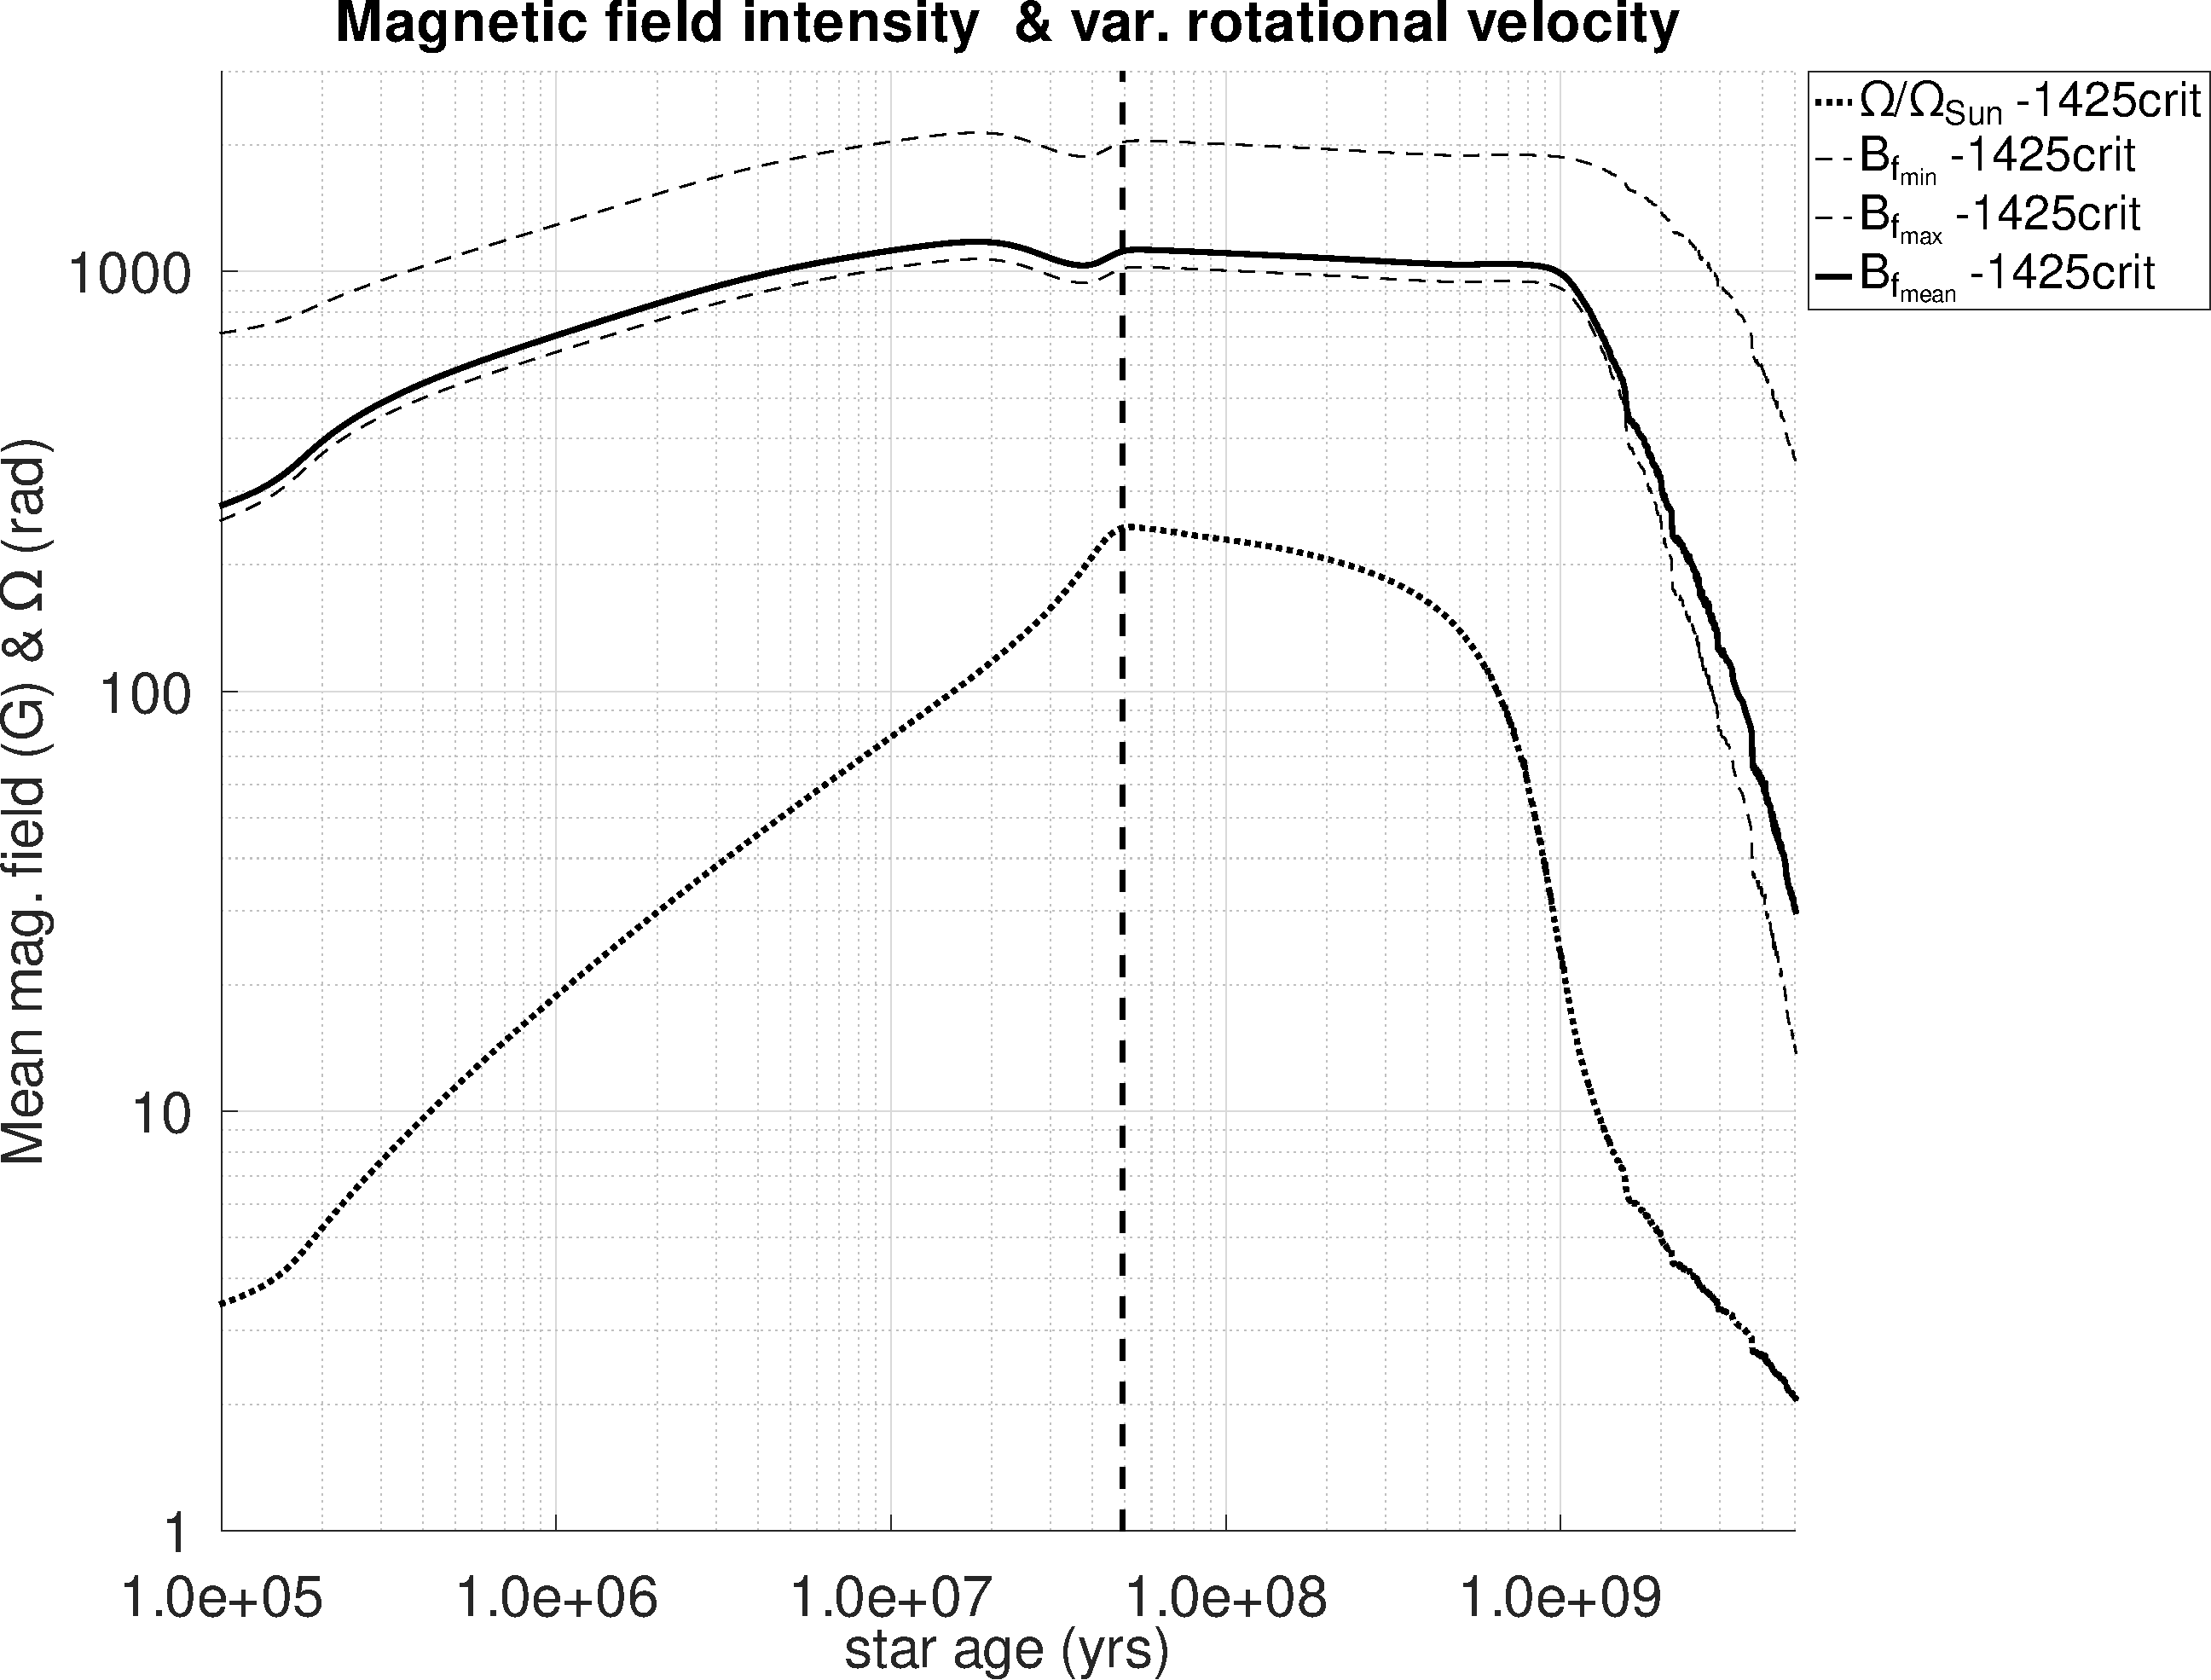
\includegraphics[clip,width=\columnwidth]{figures/paper2/mag_field_limits_var_vel_g3.pdf}
    \caption{The evolution of magnetic field intensity and its upper and lower limits, as a function of time and $\omegaini$ for a 1 $\msun$ model. The model include rotation with $\omegaini$ = 0.1425. The solid lines represent the magnetic field strength, while the dotted lines represent the angular evolution of the star. The dashed vertical line makes reference to the ZAMS.}
    \label{fig:mag_field_limits_var_vel_g3}
\end{figure}

With this formalism we are able to calculate the mean magnetic field as a time-dependent function of $\rho$, $\teff$, and $\Omega$. The time values for these three variables will be obtained from the different simulations carried out with MESA.

\subsection{Modelling magnetic braking} \label{mod_mb}
Once we have characterised how the magnetic field strength evolves, we need to model how the loss of angular momentum occurs. As the star undergoes contraction during the pre-main-sequence (PMS) phase towards the Zero-Age Main Sequence (ZAMS), its angular velocity increases, leading to a gradual augmentation in the mean magnetic field. In our analysis, we observed intensities that reached $1.0,\mathrm{kG}$, as depicted in Figure \ref{fig:mag_field_limits_var_vel_g3}. It then enters a saturation stage (although with a downward trend) up to $1.0$ Ga, and finally declines sharply as a result of the star's slower angular velocity. In contrast, our previous work in \citet{Caballero2020} employed a model suited for magnetic fields of non-variable intensity and ranging from a few Gauss ($1.0,\mathrm{G} \leq B \leq 10.0,\mathrm{G}$). The significantly higher intensities required in the present formalism render the previously employed model inadequate.\par


Let us start by enumerating the most relevant aspects and assumptions made in modeling the evolution of rotation, magnetic braking and angular momentum. If we assume a spherical outflow, the torque applied by a magnetically-coupled stellar winds $\torquewind$ is dictated by,
\begin{ceqn}
\begin{equation}
    \torquewind \propto \Omega_* \; \mwind \; \ralfven^{2} \label{eq:mb_torque}
\end{equation}
\end{ceqn}
where $\mwind$ is the mass loss rate, and $\ralfven$ the averaged value of the Alfvén radius.\par
Stars with similar initial masses but different mass loss ($\Dot{M}$) rates will end up evolving very differently. The ionized particles carried by the solar wind not only contribute to the mass loss but also to the loss of kinetic energy that is deposited in the interstellar medium. Given a star with a spherically symmetric wind, $\mwind$ is characterized by the following expression:

\begin{ceqn}
\begin{equation}
    \mwind = 4\upi r^2\rho\nu \label{eq:mass_loss}
\end{equation}
\end{ceqn}
where $r$ is the stellar radius, $\rho$ the mass density, and $\nu$ the stellar wind velocity.

It has been observed that strongly magnetic intermediate-mass stars typically have rotation rates much slower than other stars in their parent population \citep{Mathys2006}. In those stars, the magnetic fields interacts with the mass loss, where the Alfv\'{e}n radius plays an important role. $\ralfven$ is defined as the point in which the magnetic field energy density and the kinetic energy density are balanced. In case that $\ralfven$ is greater than the stellar radius, then the wind flow will have to follow the magnetic field. As a consequence, the material leaves the stellar surface with a higher specific AM, as the co-rotation radius has increased and it roughly corresponds to $\ralfven$ which can be expressed as \citep{Matt2012}
\begin{ceqn}
\begin{equation}
    \ralfven = K_1\left[\frac{\Bp^{2}\;R_*^{2}}{\mwind\;\sqrt{K_2^2\vesc^2 + \Omega_*^2R_*^{2}}\ }\right]^{m}R_*  \label{eq:mb_ralfven}
\end{equation}
\end{ceqn}
where $\Bp$ is the magnetic field intensity at the stellar surface, $\vesc$ is the escape velocity, $m = 0.1675$, $K_1 = 1.30$, and $K_2 = 0.0506$ \citep{Gallet2013}.
\begin{ceqn}
\begin{align}
\Bp &= f_*B_* \label{eq:bp}\\
\vesc &= \sqrt{\frac{2\,G\,\mstar}{\rstar}} \label{eq:vesc}
\end{align}
\end{ceqn}

Finally, we have that the AML can be calculated as follows:
\begin{ceqn}
\begin{equation}
 \Dot{J} = \Omega_* \; \mwind \; \ralfven^{2} \label{eq:j_dot}
\end{equation}
\end{ceqn}
where $\mwind$ is the mass loss rate. This expression is implemented in MESA on the basis of values directly exposed during the simulations.

\subsection{Modelling adaptive MLT $\alpha$} \label{mod_mltalpha}
The mixing-length theory (MLT) introduced by \citet{BohmVit58} has been commonly adopted to model stellar convection in stellar evolutionary codes, including MESA. The most prominent parameter in this theory is the mixing length $l$ which is defined as 
\begin{ceqn}
\begin{equation}
 l = \amlt H_p\label{eq:mixlength}
\end{equation}
\end{ceqn}
where $H_p$ is the pressure scale height, and $\amlt$ a free parameter which is determined in advance and normally keep fixed during the stellar evolution simulations.\par

 It became evident that the influence of the free parameter associated with the MLT significantly conditioned the evolution of the Li abundance. Moreover, there are no strong arguments that suggest that the mixing-length parameter is the same in all stars and at all evolutionary phases \citep{Pasetto2014}. In \citet{Caballero2020} the authors showed how an alternative mixing-length (ML) parameterization could produce results in line with the observations. Adjustment of ML over-shooting and $\amlt$ free parameter seems to be required for explaining Li abundances in OC's.\par

In \citet{Sonoi2018}, the authors introduced a way for calibrating $\amlt$ for solar-like stars in which its value increases with increasing $\gsurf$ or decreasing $\teff$. They calibrated the values of $\amlt$ for several simulated 3D models using the CO$^5$BOLD code \citep{Freytag2011} and transferred them to the 1D models developed by \citet{Ludwig1998}. The parameterization they obatained was: 

\begin{ceqn}
\begin{equation}
 f(x,y) = a_0 + (a_1 + (a_3 + a_5x +a_6y)x + a_4y)x + a_2y\label{eq:alpha_ml}
\end{equation}
\end{ceqn}
where
\begin{ceqn}
\begin{align}
     x &= \frac{\teff-5777}{1000} \label{eq:eq:alpha_x}\\
     y &= \gsurf-4.44 \label{eq:eq:alpha_y}
\end{align}
\end{ceqn}
and $a_i$ are the resulting coefficients of the fitting function to the calibrated $\amlt$ values for the MLT convection model \citep{Sonoi2018}: $a_0=1.790295$, $a_1=-0.14954$, $a_2=0.069574$, $a_3=-0.00829$, $a_4=0.013165$, $a_5=0.080333$, $a_6=-0.03306$.\par

\subsection{Grid of Models} \label{sec_grid}
Following \citet{Caballero2020} we restrict our simulations to solar-type stars with a mass of $1\,\msun$. The evolutionary models of stellar interiors incorporate rotation effects, account for the magnetic braking on stellar evolution, and track the rotational history and the surface abundance of $A(\isotope[7]{Li})$ for various initial angular velocities ($\omegaini$). The main differences lie in the parameterization of new model: we have put the focus on reducing the number of free parameters involved in the simulations. A pivotal innovation lies in the introduction of a variable magnetic field strength ($B$) and a variable $\amlt$ parameter. As for the treatment of convective overshoot mixing, a departure from the previous model is evident; we deliberately deactivate this feature in our current model. This isolates the impact of a variable $\amlt$ on A(Li) from the effects associated with convective overshooting. Notably, convective overshoot mixing is commonly addressed through ad hoc extensions of the Mixing Length Theory (MLT), introducing an additional free parameter. The Table \ref{tab:phy_mesa} enumerates the similarities and differences in the configuration of the models used in \citet{Caballero2020} and in this paper.\par

For a comprehensive overview of the similarities and differences between the configurations of the models used in \citet{Caballero2020} and the present study, refer to Table \ref{tab:phy_mesa}.


\begin{table}
\begin{threeparttable}
	\centering
	\begin{tabular}{ll} 
		\hline
		Parameter & Adopted prescriptions and values\\
		\hline
		Solar Abundance & $X_{\odot}=0.7154, Y_{\odot}=0.2703, Z_{\odot}=0.0142$\\
		Equation of State & OPAL+SCVH+MacDonald+HELM+PC\\
		Opacity & OPAL Type I for log T $\geq$ 4 \\ & Ferguson for logT $<$ 4\\
		Reaction Rates & JINA REACLIB\\
		Boundary Conditions & ATLAS12; $\tau$=100 tables + photosphere\\
		Diffusion & Track \isotope[1]{H}, \isotope[2]{He}, \isotope[7]{Li}, \isotope[7]{Be}\\
		Rotation Schema & Differential rotation at PMS \& MS\\ & Include SH\tnote{1}  , ES\tnote{2}  , GSF\tnote{3}  , SSI\tnote{4}  , DSI\tnote{5}\\
		Thermohaline & $\alpha_{{\rm th}}=666$\\
		\textbf{Convection} & $\alpha_{{\rm MLT}}$ variable depending on $\teff$\\ & \& $\gsurf$ + Ledoux\\
            Semiconvection & $\alpha_{{\rm sc}}=0.1$\\
		\textbf{Overshoot} & $f_{{\rm ov,core}}=0.0$, \& $f_{{\rm ov,sh}}=0.0$\\
		\textbf{Magnetic Field} & B(G) variable, depending on $\rho$, $\teff$ \&  $\Omega$\\
		Mass Loss & $\Dot{M}_{{\rm max}} = 10^{-3} \: \msun \: yr^{-1}$\\
		Angular Moment Loss & $\Dot{J} = \Omega_* \; \mwind \; \ralfven^2$\\
		\hline
	\end{tabular}
    \begin{tablenotes}\footnotesize
        \item (1) Solberg-Hoiland, (2) Eddington–Sweet
        \item (3) Goldreich–Schubert–Fricke, (4) Secular Shear Instability
        \item (5) Dynamical Shear Instability
    \end{tablenotes}
    \end{threeparttable}
    \caption{Summary of adopted physics in MESA \citep[based on][]{Choi2016,Caballero2020}. Highlighted in bold are the parameters with different configuration from referenced works.}
	\label{tab:phy_mesa}

\end{table}

The models include rotation since the PMS. We computed the evolution of $1\,\msun$ stellar models at solar initial metallicity with $\omegaini = \oomegac$ varying between $0.12$ and $0.1425$. We have adopted the following theoretical approach to establish when the star is reaching the ZAMS: as both the central \isotope[1]{H} mass fraction has been reduced by $\Delta( \isotope[1]{H})= 0.0001$ from its initial value, and the star's luminosity ($L$) is almost fully ($L \geq 0.99$) generated by the nuclear reactions of \isotope[1]{H} occur simultaneously. The results are then compared with the stellar ages from stars in OCs collected by the Gaia mission and GES and referenced in Table \ref{tab:oc_reduced_list}.\par

As expressed by Eq.~\ref{eq:mb_torque}, the amount of AML depends on $\ralfven$, $\Omega$ and $\Dot{M}$. For large $\ralfven$ values, the star undergoes a significant deceleration. The value of $\ralfven$ depends on the following varying parameters: magnetic field ($B$) intensity, $\teff$ and $\Omega$. With regards to $\Dot{M}$ and as reported in Table \ref{tab:phy_mesa}, the empirical formula developed by Reimers \citep{Reimers1975} for stars in the asymptotic giant branch (AGB) was used for calculating the mass-loss. For a solar-type star the $\Dot{M}$ during MS is relatively small, about  $10^{-14}\msun \, yr^{-1}$ \citep{Noerdlinger2008}. \par

MESA assigns an $\Omega$ value for each cell $k$ ($\Omega_k$) which is adjusted so that the resulting angular momentum is retained after calculating the new mass of the cell $k$ ($m_k$) and its distance to the center of the star ($r_k$). After that, an AM value is assigned to each cell $k$ ($J_k$). At this point, our MB routine will turn on if the star has both an extensive convective layer, and a radiative core. From this moment on, the MB routine was activated, acting as an additional mechanism to those existing in the MESA evolutionary code that participated in the star AML and modifying $J_k$. This was done by providing an additional contribution ($\Dot{J}_{k}$). This contribution is the result of the external torque exerted by the magnetic field once it has been distributed among the different layers that make up the CZ as dictated by Eq.~\ref{eq:k_jdot}:\par
 
\begin{ceqn}
\begin{align}
    \Dot{J}_{k} &= \Dot{J}_*\;\frac{m^{}_{k} r^2_{k}}{m^{}_* r_*^2} \label{eq:k_jdot}
\end{align}
\end{ceqn}

\section{Results} \label{sec_3}
There are evidences that advocate for a strong established relationship between Li destruction and stellar rotation, so that the higher the angular velocity, the more Li destruction occurs (see \citet{Bouvier2018, Caballero2020}). The effect of the MB on the time evolution of A(Li) is given by its ability to remove AM from the star, and thus influence its rotational velocity, causing the star to rotate more slowly and to destroy less Li.\par

In Figure \ref{fig:li_var_vel_var_g_3} it is shown the temporal evolution of surface Li abundance for several 1 $\msun$ models. Those models were initialized with different rotational velocities and took into consideration the effects of MB caused by a variable magnetic field. If we compare it with Figure \ref{fig:li_var_vel_0g} in which the effects of MB were neglected, we notice how the profiles of Li abundance were altered across PMS and MS. During the PMS we can describe the effect as modest, somewhat expected and in line with the fact that the AML caused by MB (see Eq.~\ref{eq:j_dot}) depends directly on the the $\Omega$ evolution and mass loss rate. If we take into account that for solar-type stars the models predict a modest total mass loss rate, that value is even much lower in this phase. It is in the approach phase to the ZAMS that the angular velocity reaches its maximum. This, according to our model, plays a crucial role in both the mass loss and the magnetic field strength. The higher the $\Omega$, the higher the $\Dot{M}$  (see Figure \ref{fig:mdot_var_vel_g3}), and the higher the magnetic field strength (see Figure \ref{fig:mag_field_var_vel_g3}). These effects combine and lead to an accentuation of the magnetic braking effect. As a consequence, there is a slowing down of Li destruction once the models enter the MS. The results of our simulations for those models respectively initialized to $\omegaini$ = 0.14 and 0.1425 reproduce A(Li) in line with that of the Sun surface \isotope[7]{Li} abundance  (1.1 $\pm$ 0.1 dex). The latter gives a value of 1.133 dex, which would represent a deviation of about 3\% from the nominal value (see Figure \ref{fig:li_var_vel_var_g_3}).\par

\begin{figure}
	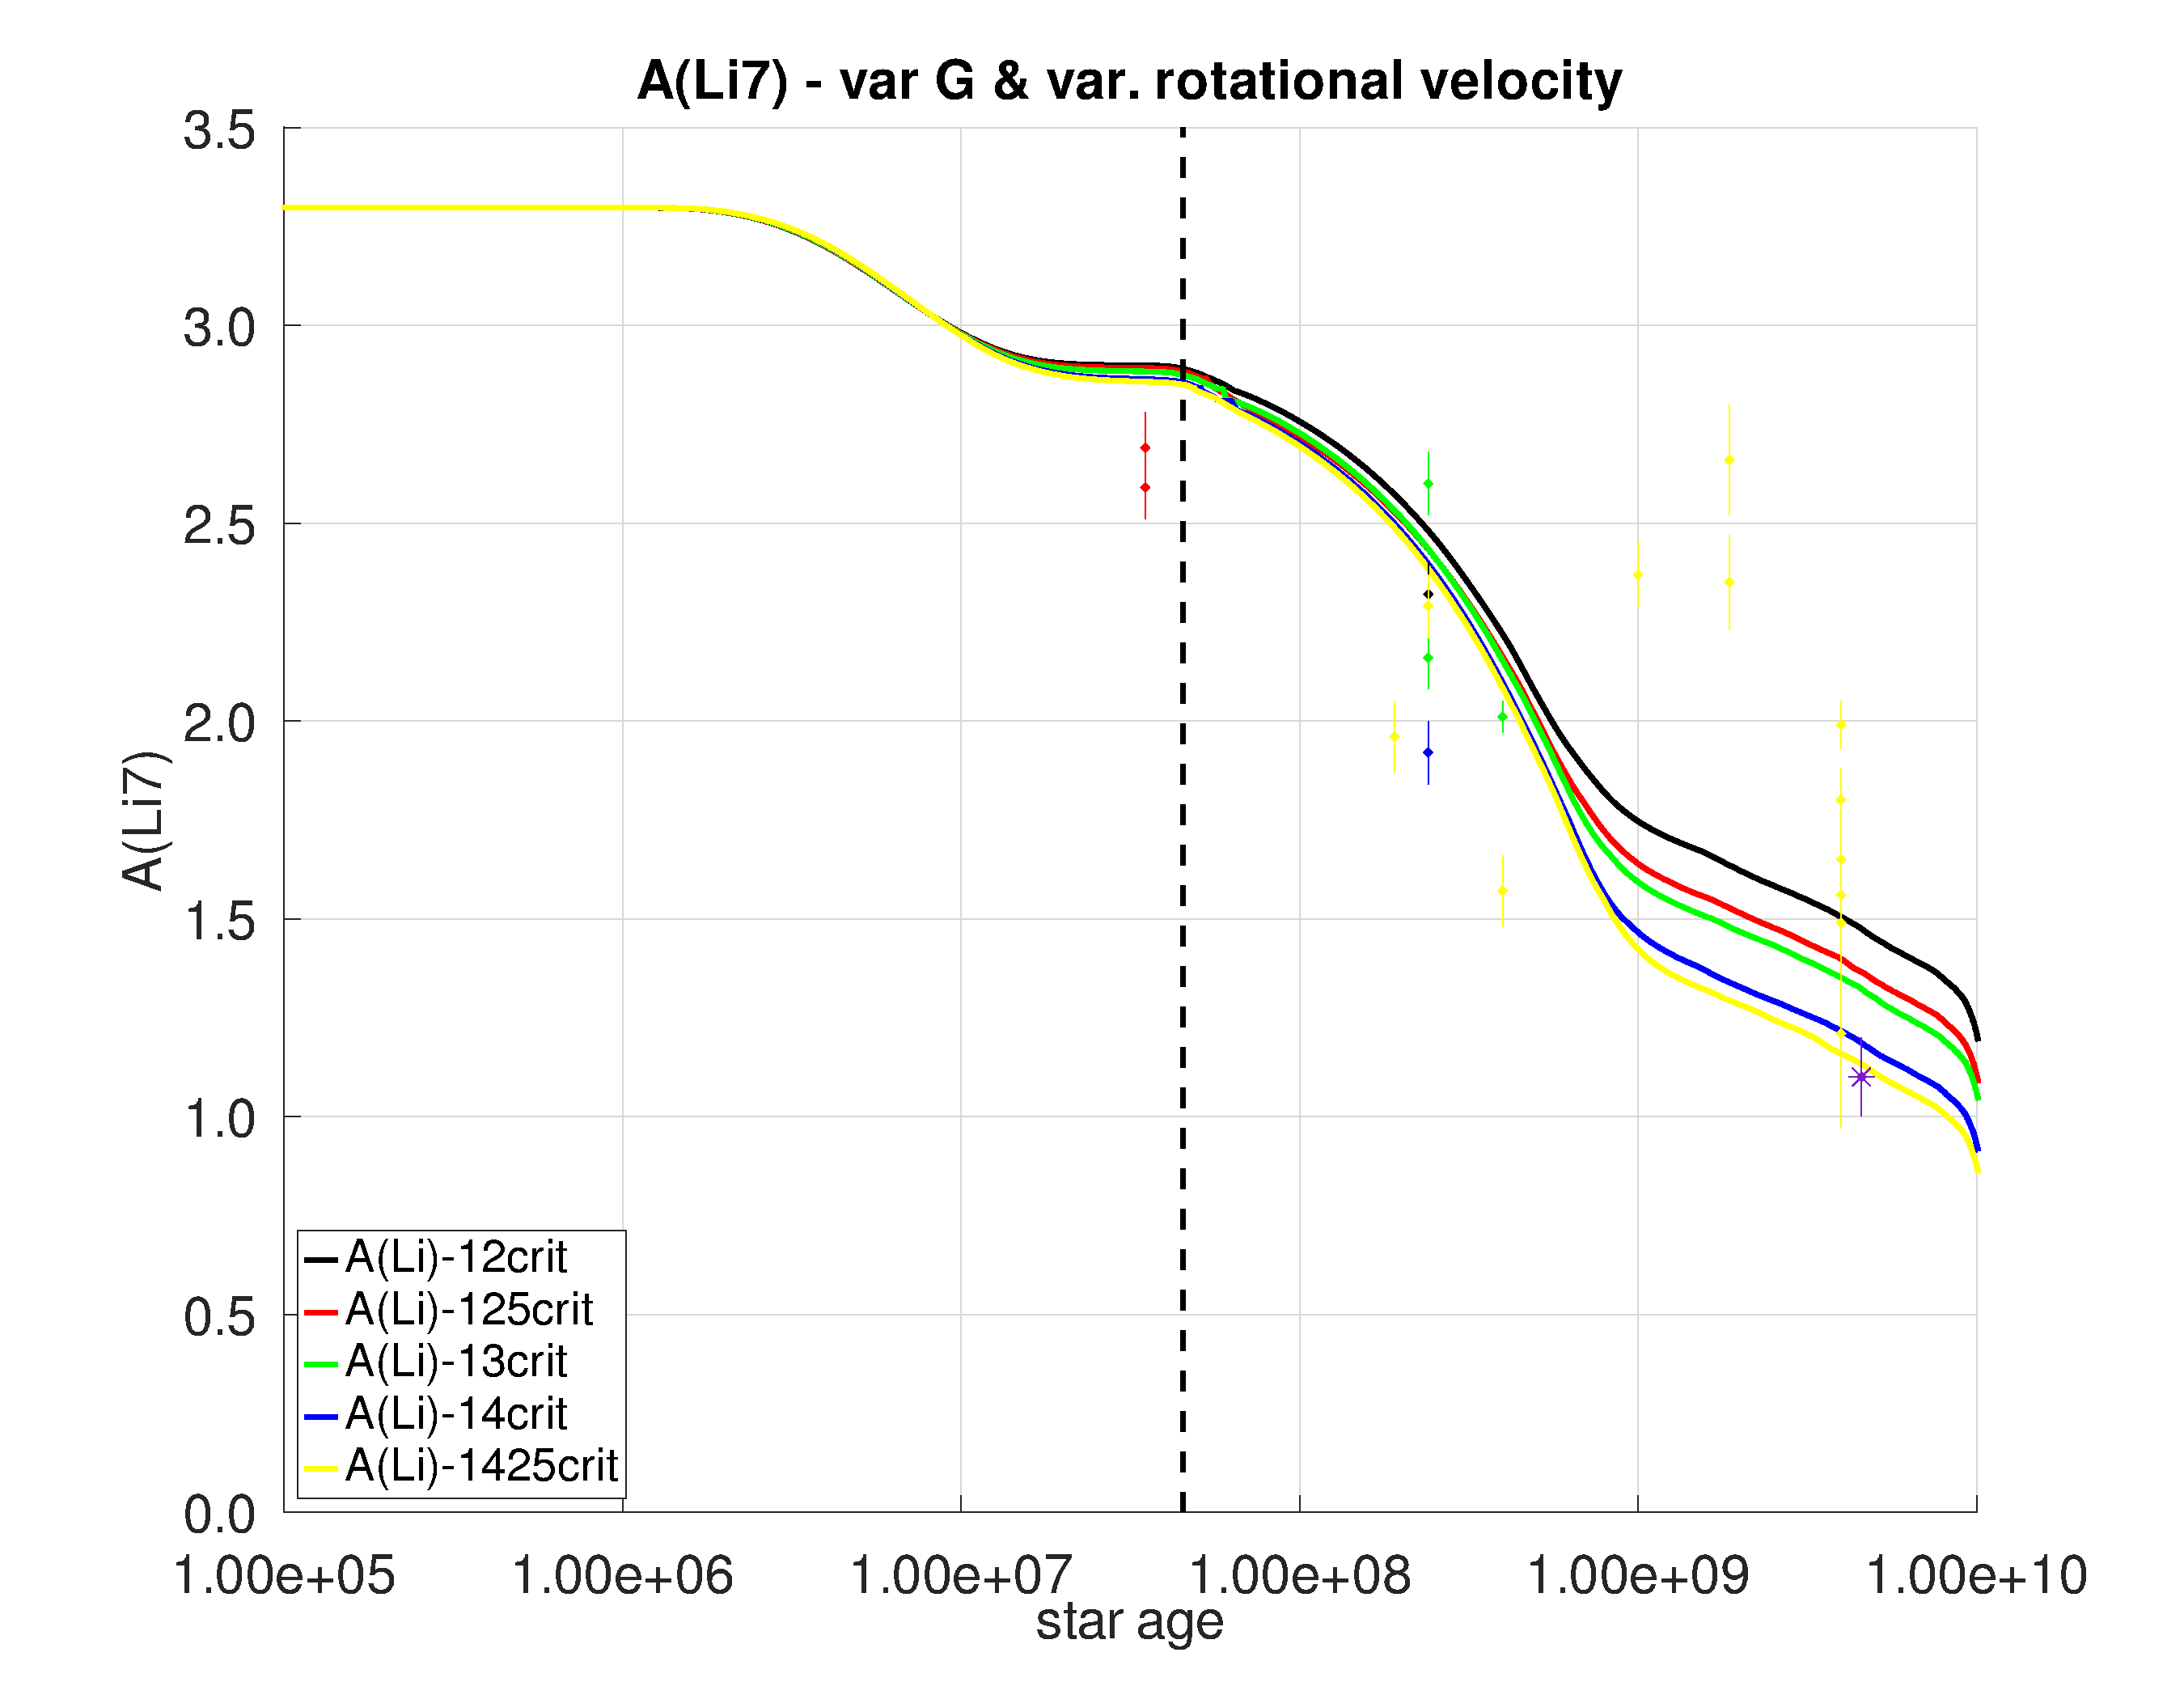
\includegraphics[clip,width=\columnwidth]{figures/paper2/li_var_vel_var_g_3.pdf}
    \caption{Evolution of the relative surface abundance of \isotope[7]{Li} compared to \isotope[1]{H} is shown for various 1 $\msun$ models. These include a magnetic field with varying intensity, initial rotation rates ranging from 0.12 to 0.1425 $\omegaini$, and MB. The purple star represents the present-day Sun's surface Li abundance \citep{Asplund2009}. The other colored dots represent surface \isotope[7]{Li} abundances for stars with parameters within the specified selection intervals, corresponding to the evolution curve of the same color. The dashed vertical line indicates the Zero Age Main Sequence (ZAMS).}
    \label{fig:li_var_vel_var_g_3}
\end{figure}

\begin{figure}
	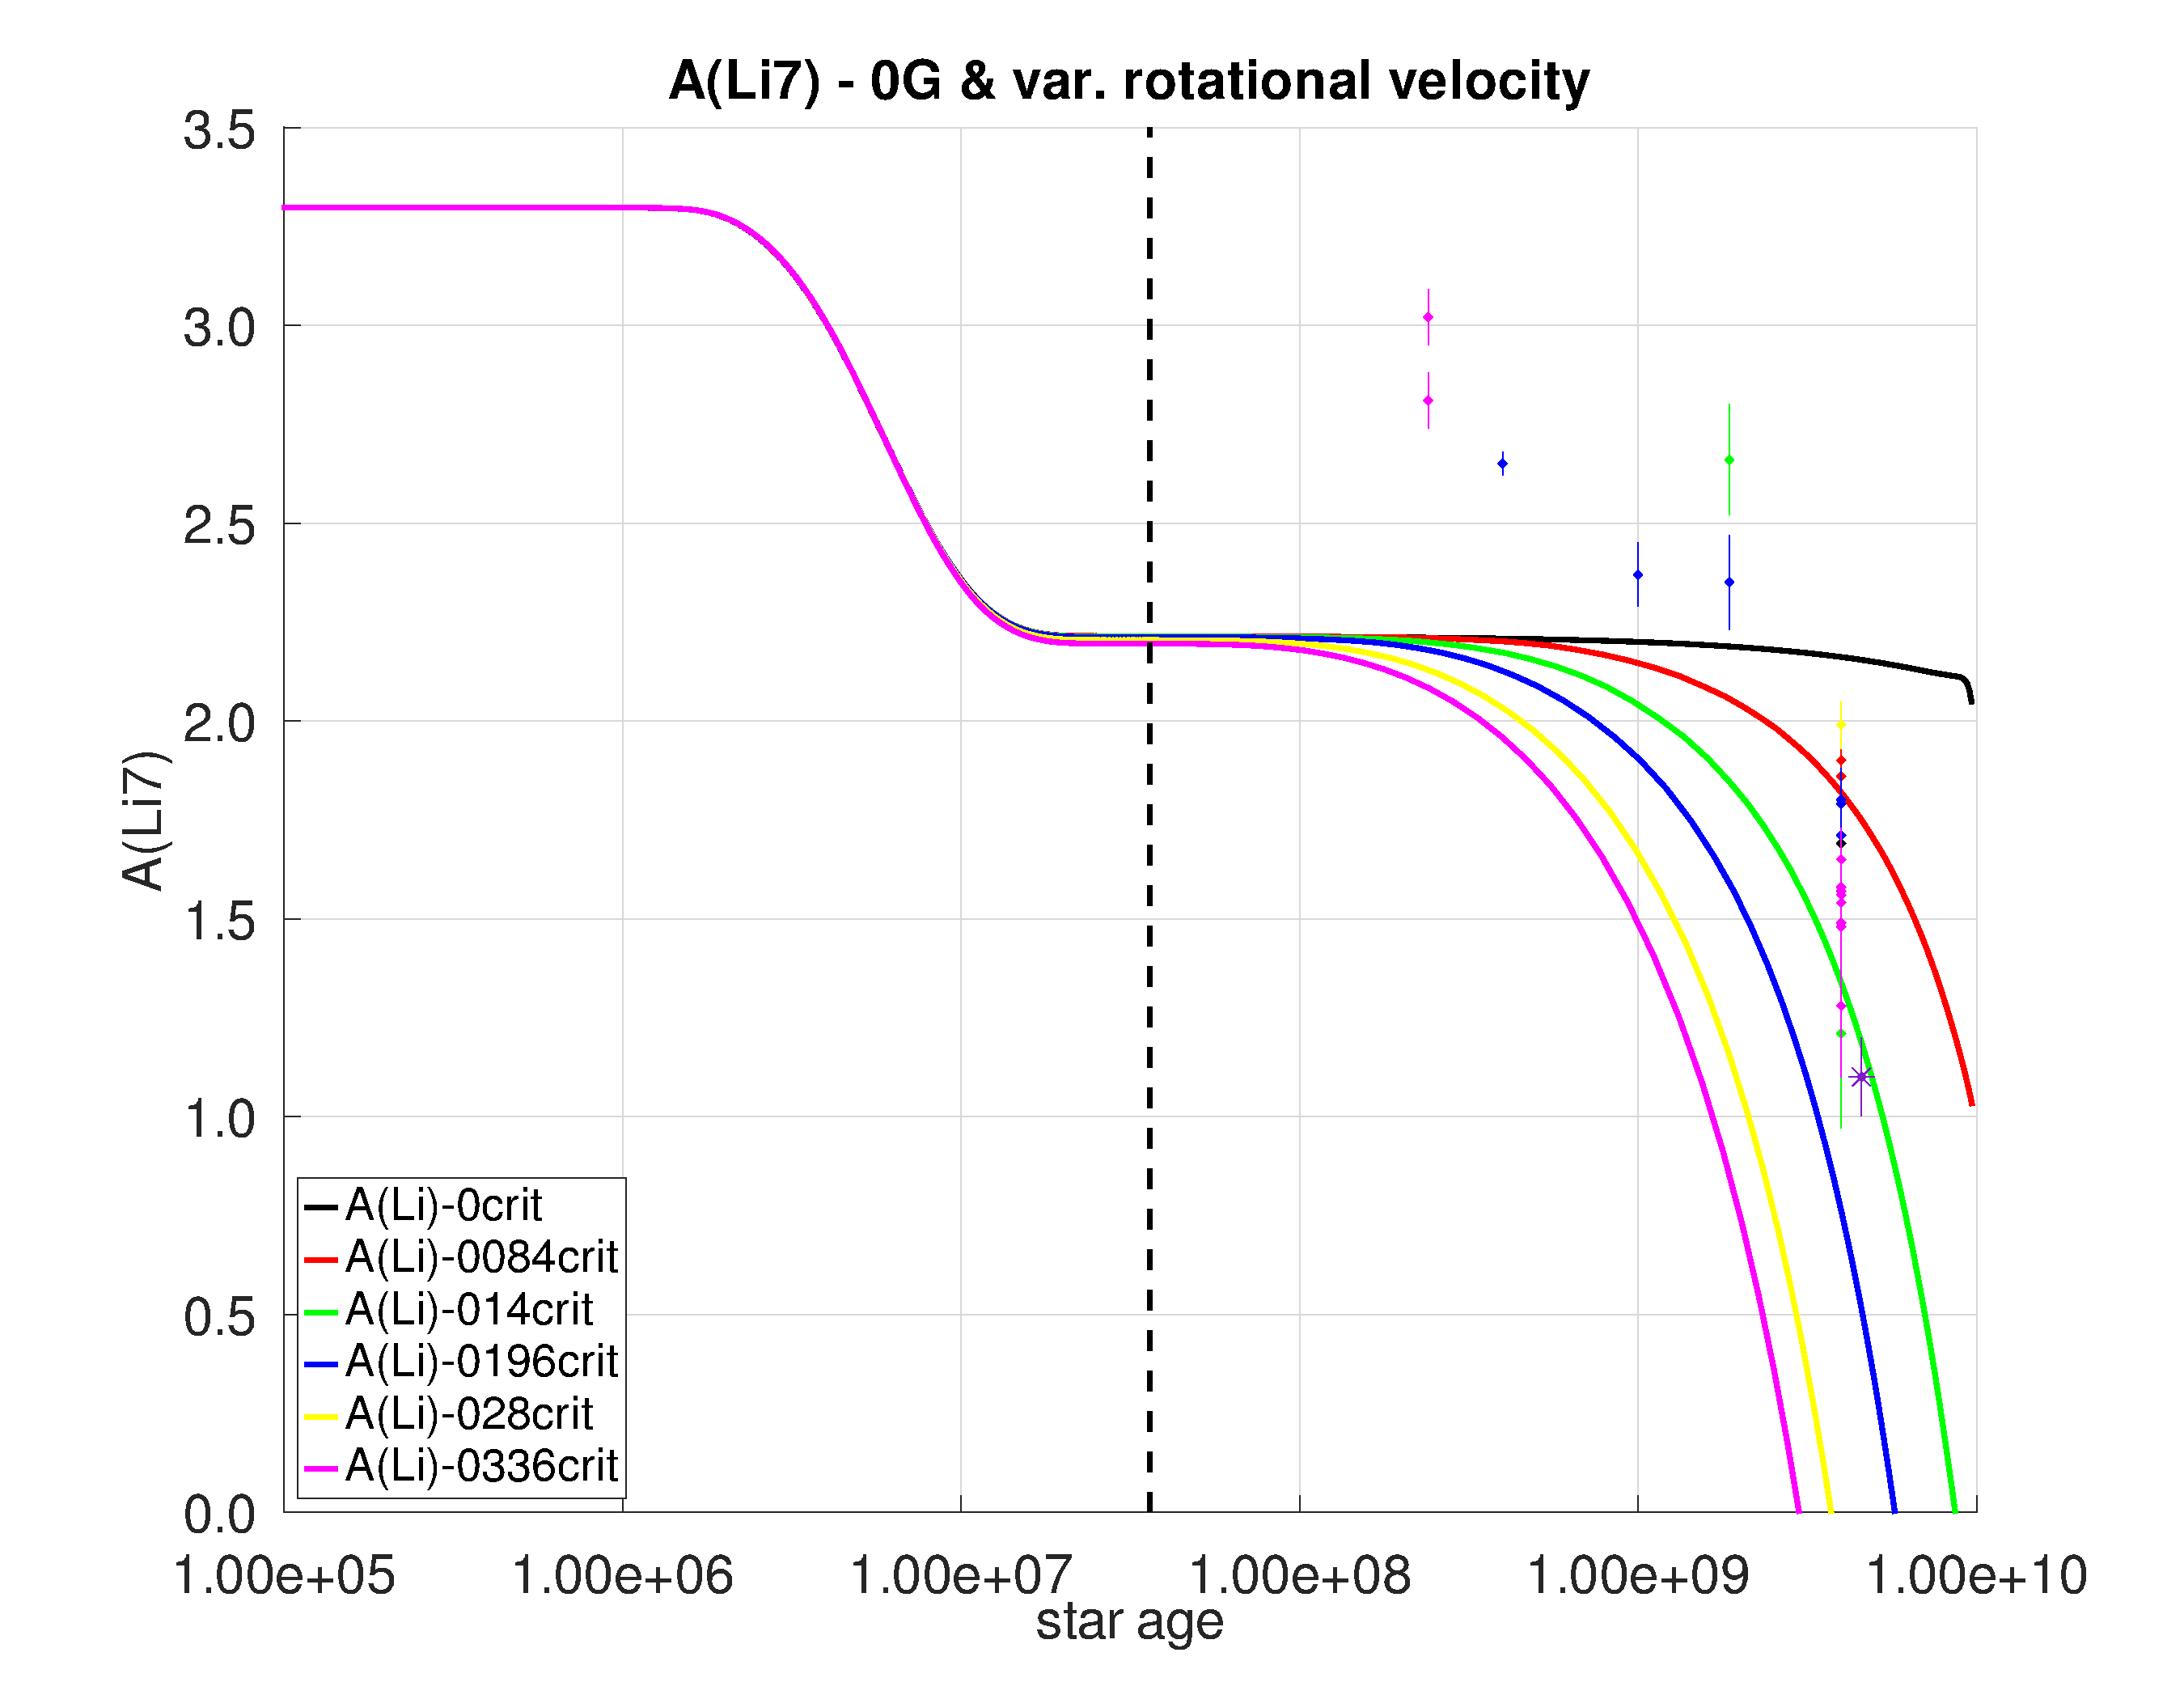
\includegraphics[clip, width=\columnwidth]{figures/paper2/li_var_vel_0_0g_0.pdf}
    \caption{Ratio of surface \isotope[7]{Li} abundance to \isotope[1]{H} as a function of time is depicted for various 1 $\msun$ models without magnetic field. The reference model, as proposed by \citet{Choi2016}, is represented by the solid black line. Additional models with initial rotation rates ranging from 0.0084 to 0.0336 are illustrated by the remaining lines. The surface Li abundances for the present-day Sun, indicated by a purple star, are based on the study by \citet{Asplund2009}. The dashed vertical line indicates the Zero Age Main Sequence (ZAMS).}
    \label{fig:li_var_vel_0g}
\end{figure}

\begin{figure}
	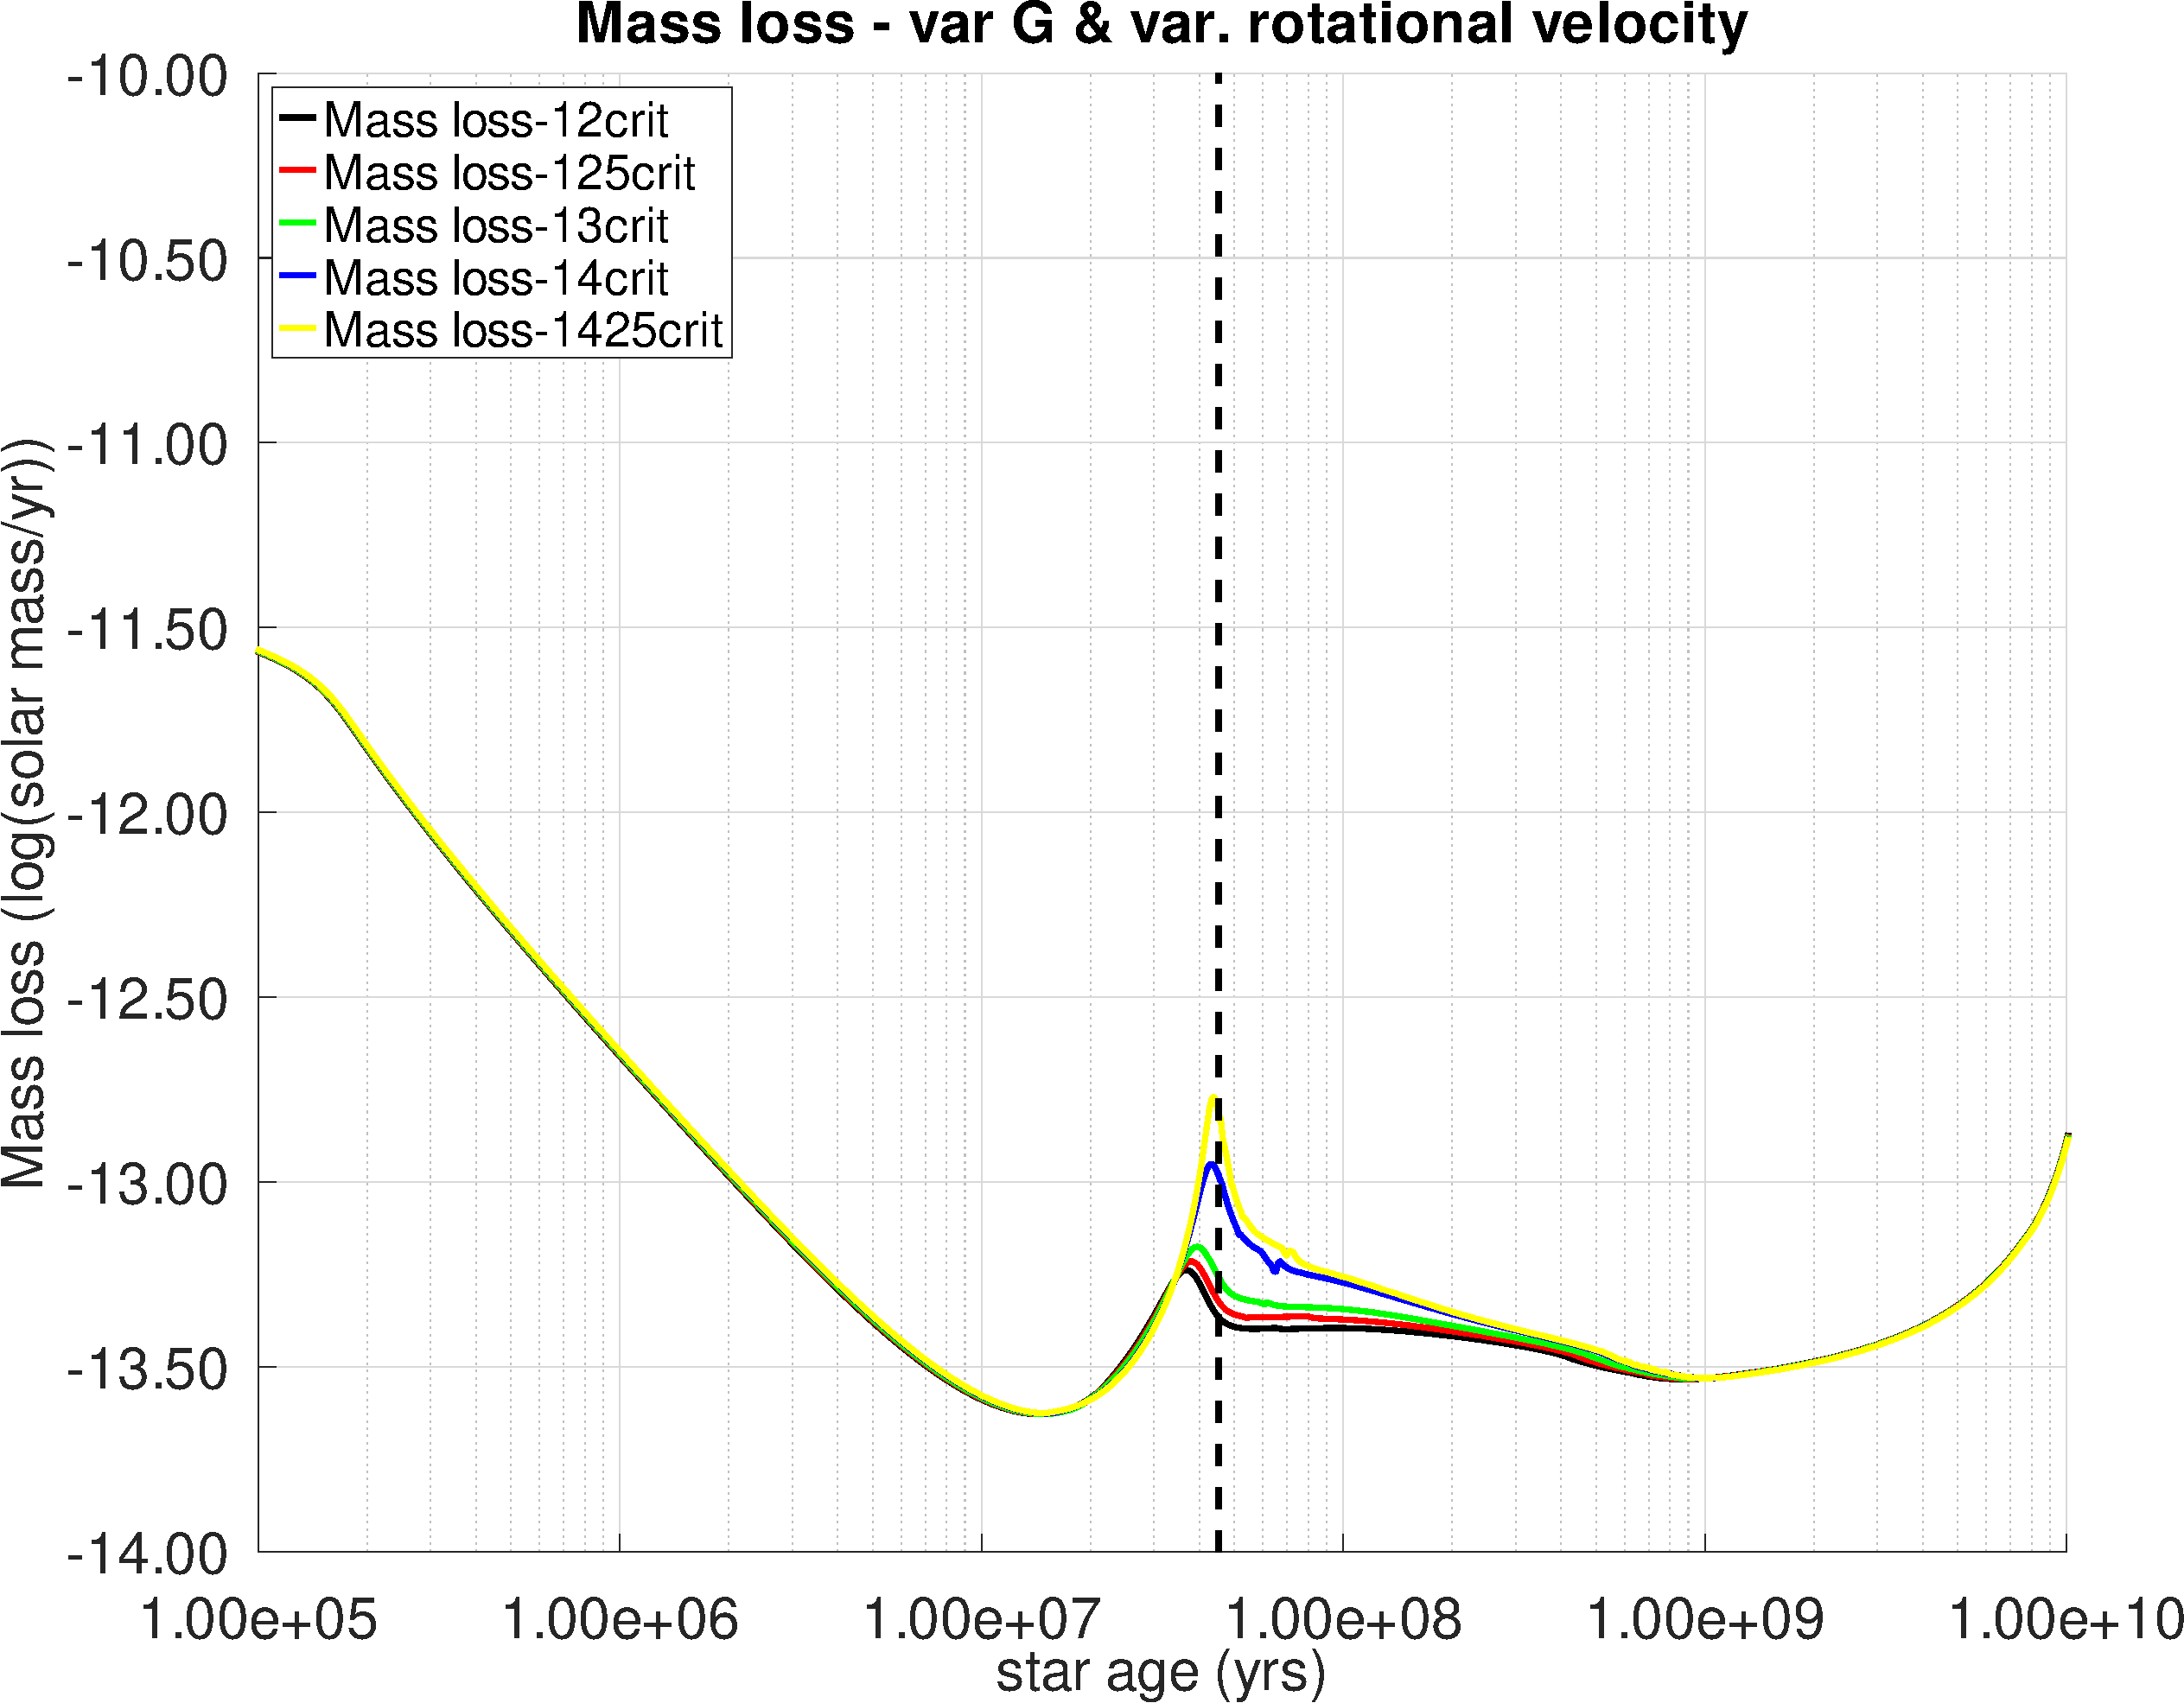
\includegraphics[clip,width=\columnwidth]{figures/paper2/mdot_var_vel_g3.pdf}
    \caption{The evolution of mass loss $\Dot{M}$ as a function of time for several 1 $\msun$ models. The models include variable magnetic field intensity and initial rotation with $\omegaini$ between 0.12 and 0.1425. The dashed vertical line makes reference to the ZAMS.}
    \label{fig:mdot_var_vel_g3}
\end{figure}


\begin{figure}
	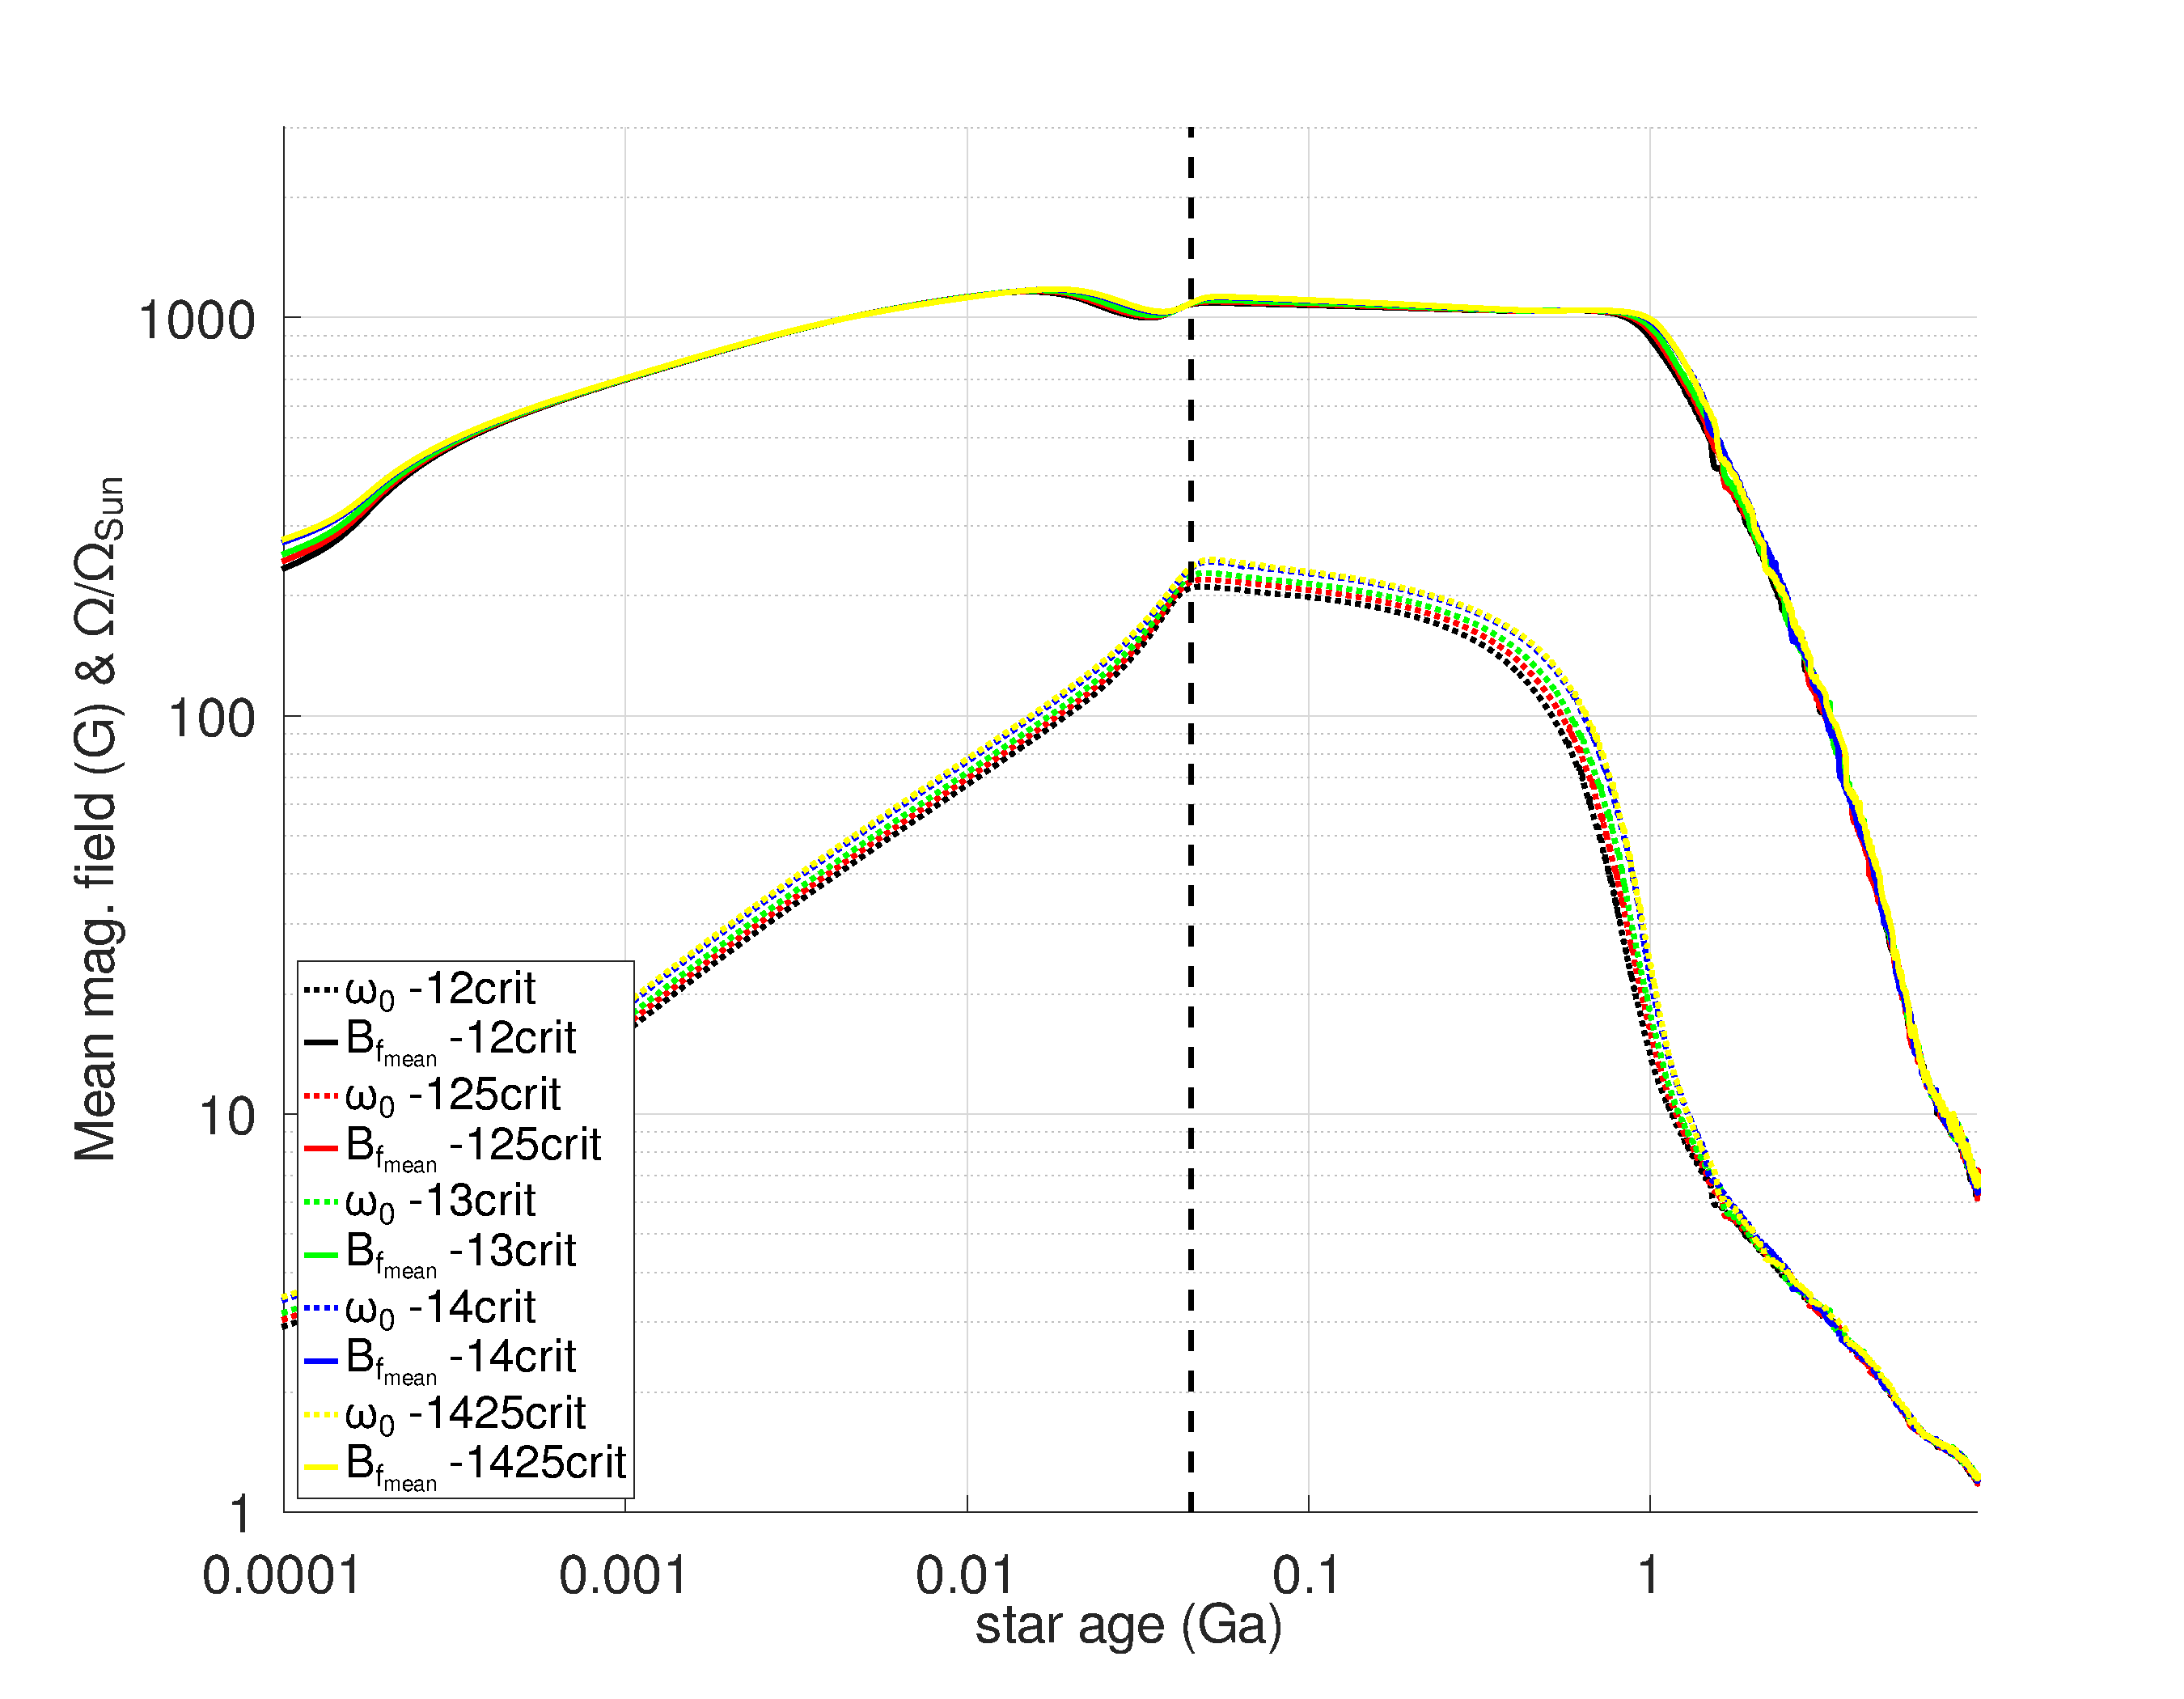
\includegraphics[clip,width=\columnwidth]{figures/paper2/mag_field_var_vel_g3.pdf}
    \caption{The evolution of magnetic field intensity, as a function of time and $\omegaini$ for several 1 $\msun$ models. The models include initial rotation with $\omegaini$ between 0.12 and 0.1425. The solid lines represent the magnetic field strength, while the dotted lines represent the angular evolution of the star. The dashed vertical line makes reference to the ZAMS.}
    \label{fig:mag_field_var_vel_g3}
\end{figure}

In Figure \ref{fig:rot_vel_var_vel_var_g3} we depict the rotation profiles of stars for the surface and for the bottom of the convective envelop. It shows how the angular velocity increases in value as the star decreases in radius along the PMS. During this stage of its evolution, the star has a nearly convective structure, as can be seen in Figure \ref{fig:cz_var_vel_var_g3}. As it approaches an age of $\approx 10^6$ years, the convective zone of the star begins to shrink in size and the core of the star reaches the temperature, pressure and density conditions necessary to develop a radiative core. In turn, the difference in the angular velocities of the different models becomes more evident, being higher in those that were initialised with a higher initial angular velocity. This fact implies that the mass loss is also higher for those stars that rotate faster. As we have described above, a larger mass loss also implies a larger angular momentum loss. The combined effects of the increases in effective temperature, angular velocity and mass loss cause the magnetic field strength to reach its maximum in the approach phase of the ZAMS (see Figure \ref{fig:mag_field_var_vel_g3}). We observed that the models with lower angular velocity generally ended up exhibiting higher values for the Li abundance on the surface (see Figures~ \ref{fig:li_var_vel_var_g_3}, \ref{fig:grid_li_var_vel} \& \ref{fig:grid_li_var_g}).\par

For the models in which we obtain values of A(Li) in line with those of the Sun ($\omegaini$ = 0.14 and 0.1425), we have on the other hand measurements for the $\Omega$ and $B$ which are not are not in tune with the respective solar ones. The Sun surface rotational velocity is 2km/s with a minimum error of 3m/s, and the mean magnetic field strength is 1G. For the simulation with $\omegaini$=0.1425, we obtain a rotational velocity at equator of 4.72 km/s. Although it is a measure on the same order of magnitude, it represents a 235\% deviation. For the average magnetic field strength we have 36.9G, far away from the reference value.\par

As described in section \ref{mod_mb}, the MB routine, which is activated when the star develops a radiative core and a convective zone above it (see Figure \ref{fig:mb_act_var_vel_g3}), distributed the total amount of AML calculated according to Eq.~\ref{eq:k_jdot} among the different layers that composed the CZ. In Figure \ref{fig:cz_var_vel_var_g3} we can observe the evolution of the most external CZ normalized with respect to the radius of the star for several 1 $\msun$ models. In accordance with the established models of stellar evolution, in a solar-type star the CZ covers practically all of it for a large part of the PMS. From the ZAMS on-wards, its size starts to decrease gradually in a first phase and then becomes more pronounced at around $4.0x10^8$ years of age. As can be seen in Figure \ref{fig:rot_vel_var_vel_var_g3}, the star, after reaching its maximum angular velocity when passing the ZAMS, starts to decelerate due to magnetic braking.\par

It is the presence of the MB that prevents the star from further increasing its angular velocity. In this way, the Li destruction is attenuated by a lower rotational velocity. The models start to decelerate gradually once the ZAMS is passed and during the initial period of their stay in the MS. The magnetic field strength remains close to its maximum, decreasing slightly and then decreasing more sharply. Its behaviour reflects that of the evolution of the angular velocity, a consequence of the effects of the MB. The deceleration process continues progressively until, around the present age of the Sun, we obtain angular velocity values very similar to the Sun. The deceleration leads to a reduced effect of centrifugal forces, which allows for a contraction of the star's radius, and thus a smaller size of the CZ. Additionally, a lower angular velocity has an effect on the magnetic field strength, as can be seen in Figure \ref{fig:mag_field_var_vel_g3}. The coupling between angular velocity, magnetic field strength, and star radius is evident and consistent.\par

\begin{figure}
	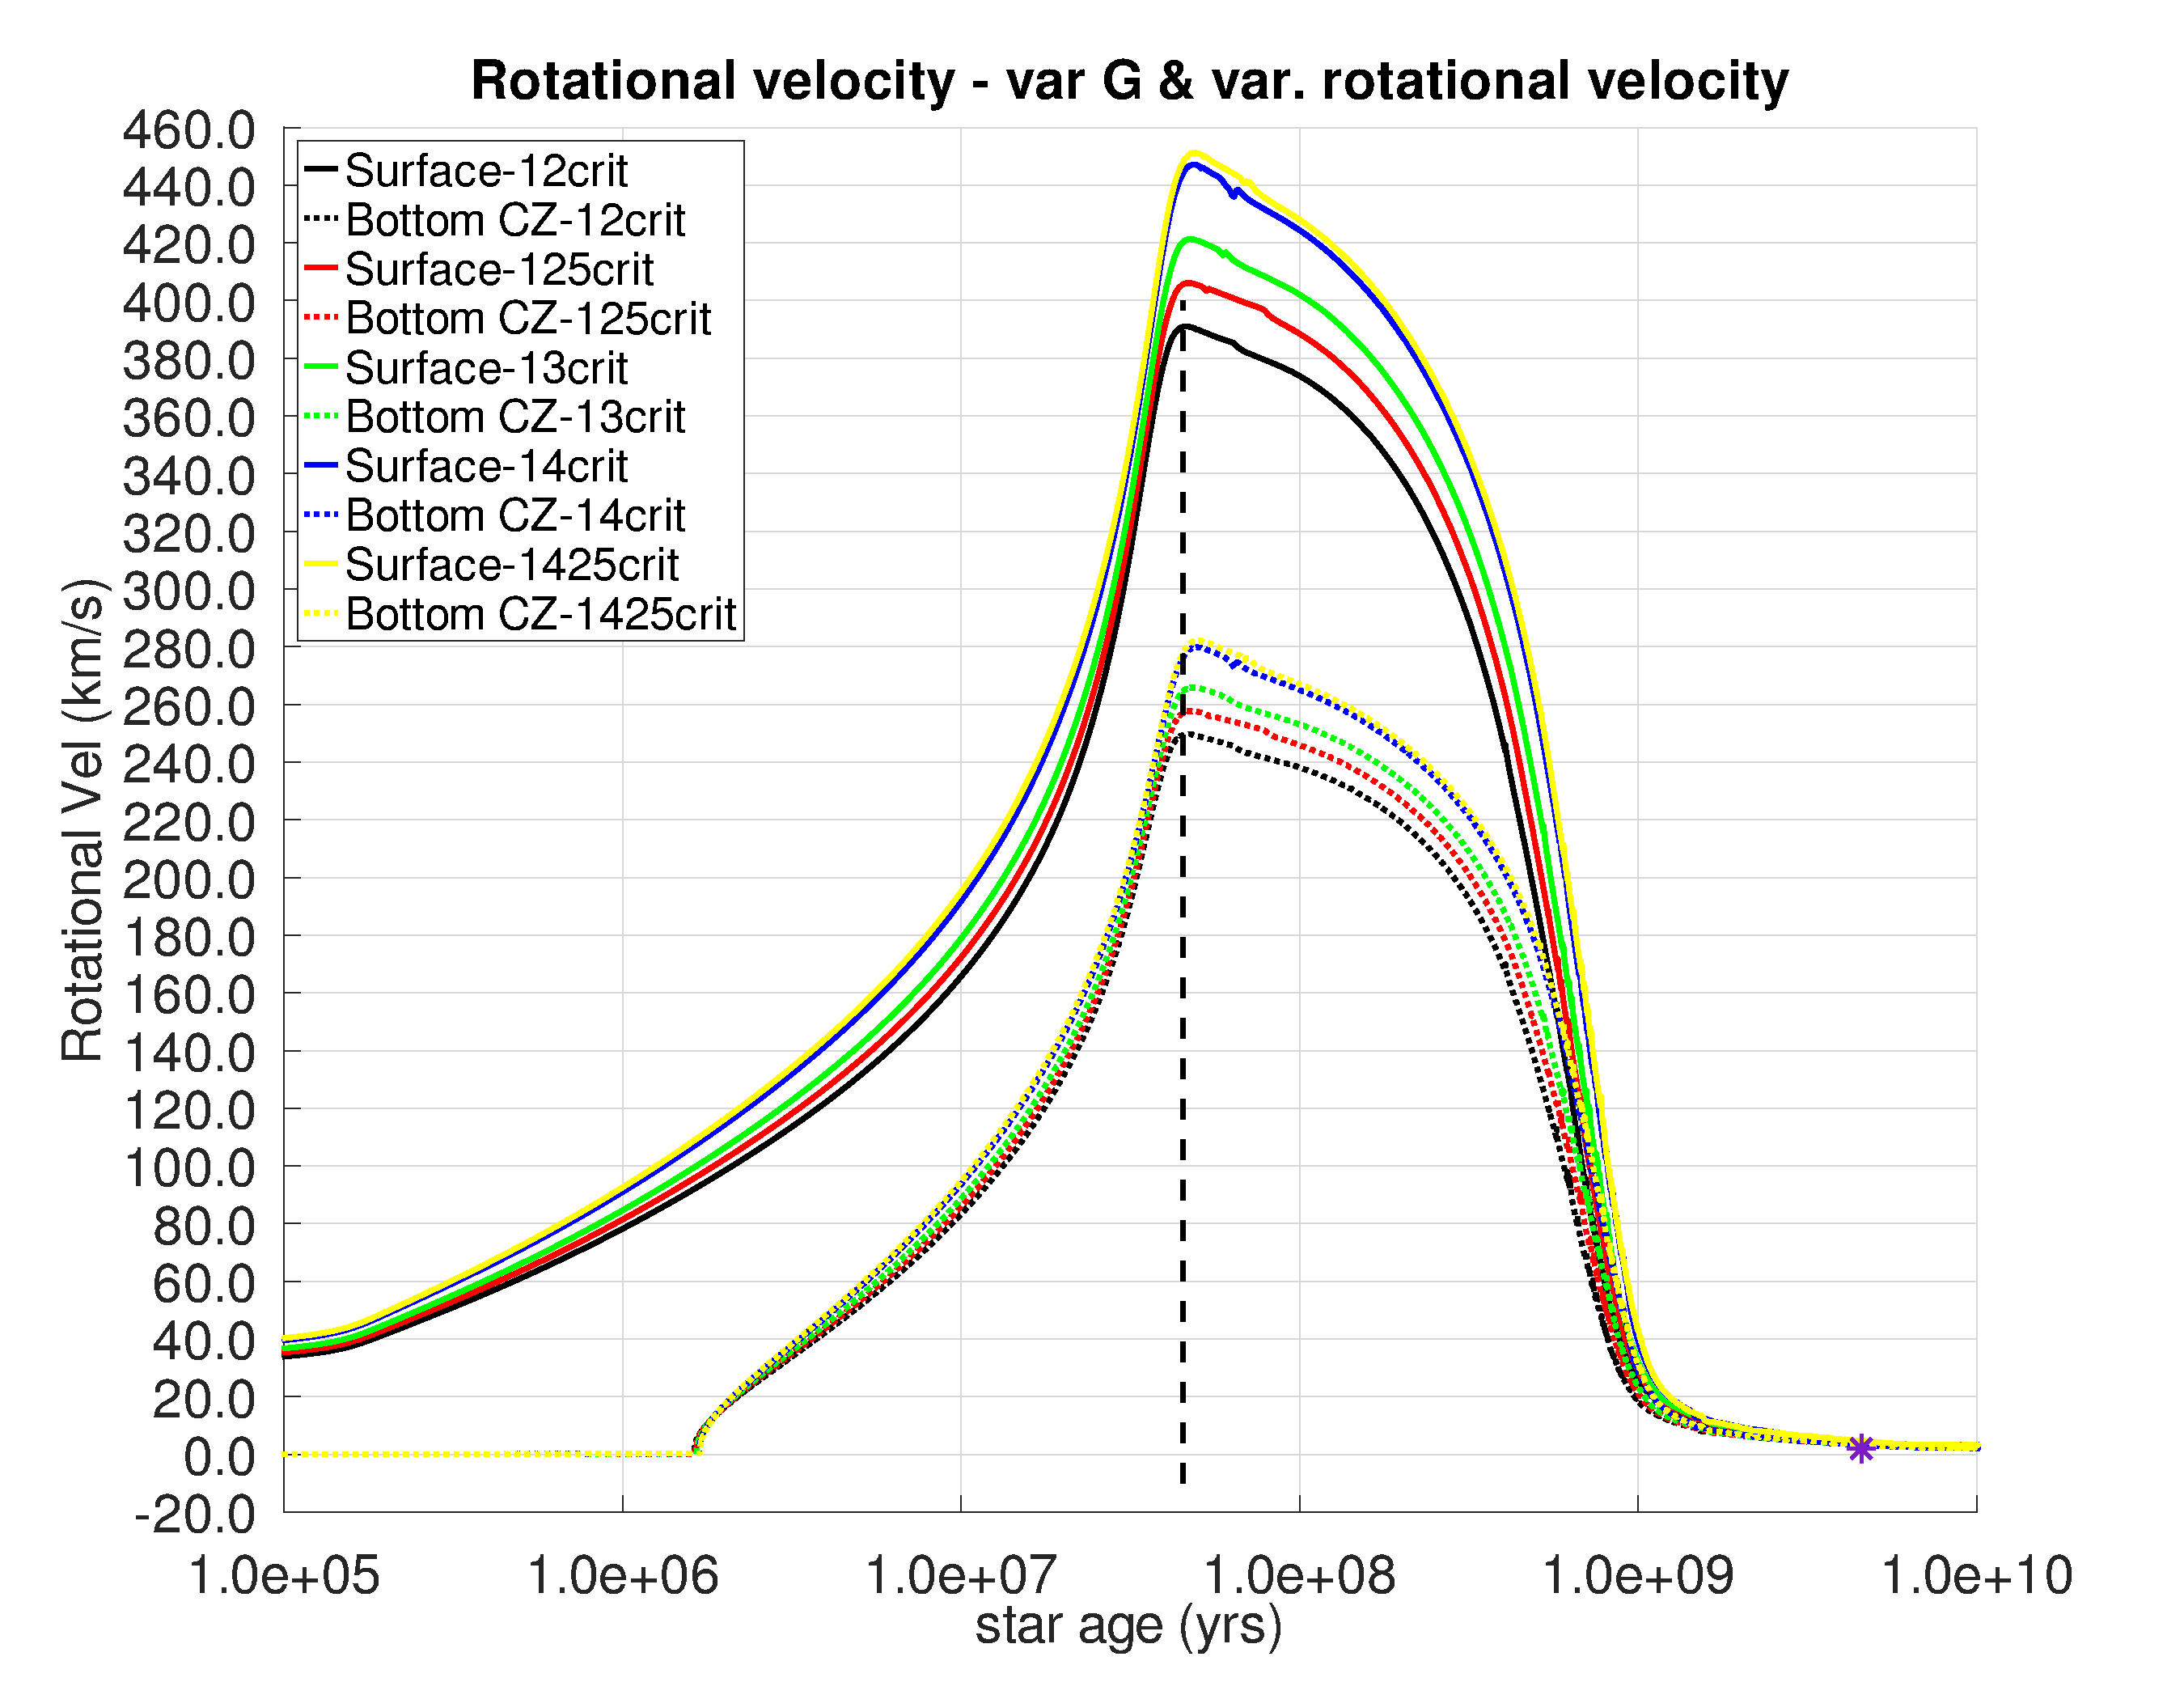
\includegraphics[clip,width=\columnwidth]{figures/paper2/rot_vel_var_vel_var_g3.pdf}
    \caption{The evolution of surface rotational velocity, as a function of time for several 1 $\msun$ models. The models include a magnetic field with variable intensity, initial rotation with $\omegaini$ between 0.12 and 0.1425, respectively and MB. The purple star is the surface angular velocity for the present-day Sun \citep{Gill2012}. The dashed vertical line makes reference to the ZAMS.}
    \label{fig:rot_vel_var_vel_var_g3}
\end{figure}

\begin{figure}
	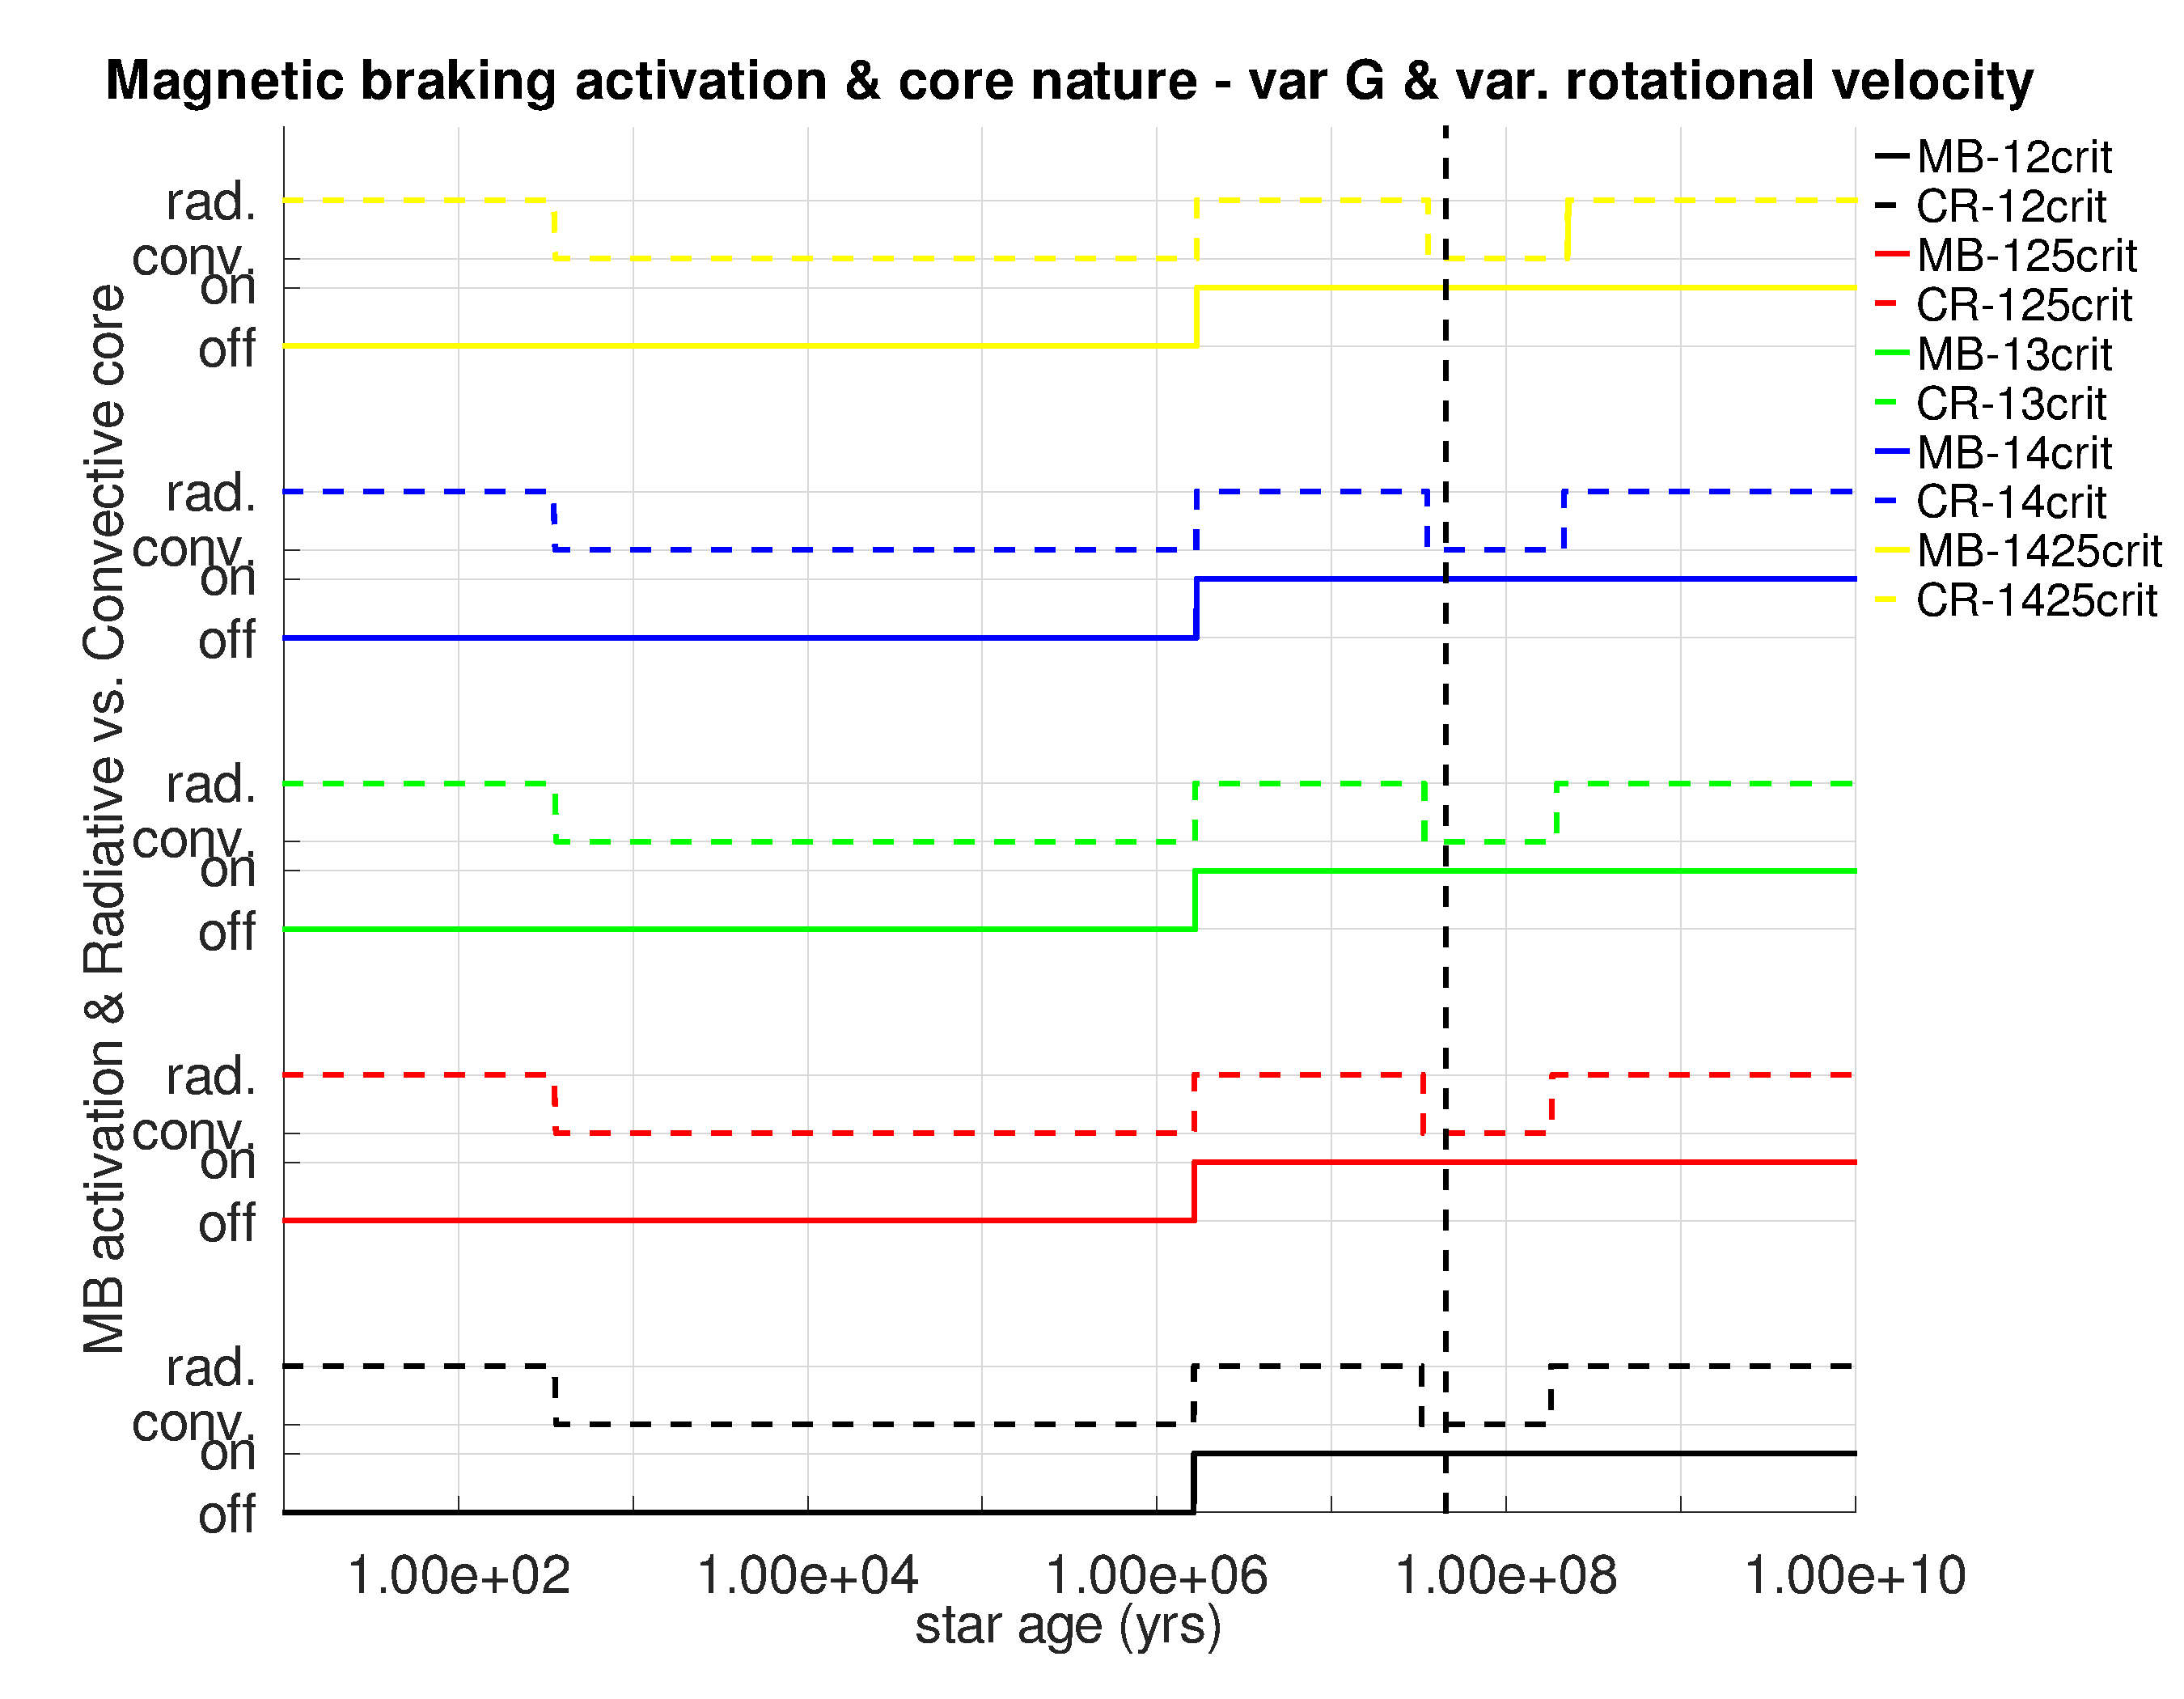
\includegraphics[clip,width=\columnwidth]{figures/paper2/mb_act_var_vel_g3.pdf}
    \caption{The activation of the magnetic braking routine as a function of the presence of a radiative core. The solid lines signal the magnetic braking routine activation (on) and deactivation (off). The horizontal dashed lines inform about the star's core nature: radiative (rad) or convective (conv). By implementation decision, once the routine is activated, it remains on even if the star's core nature change to convective. The dashed vertical line makes reference to the ZAMS.}
    \label{fig:mb_act_var_vel_g3}
\end{figure}

\begin{figure}
	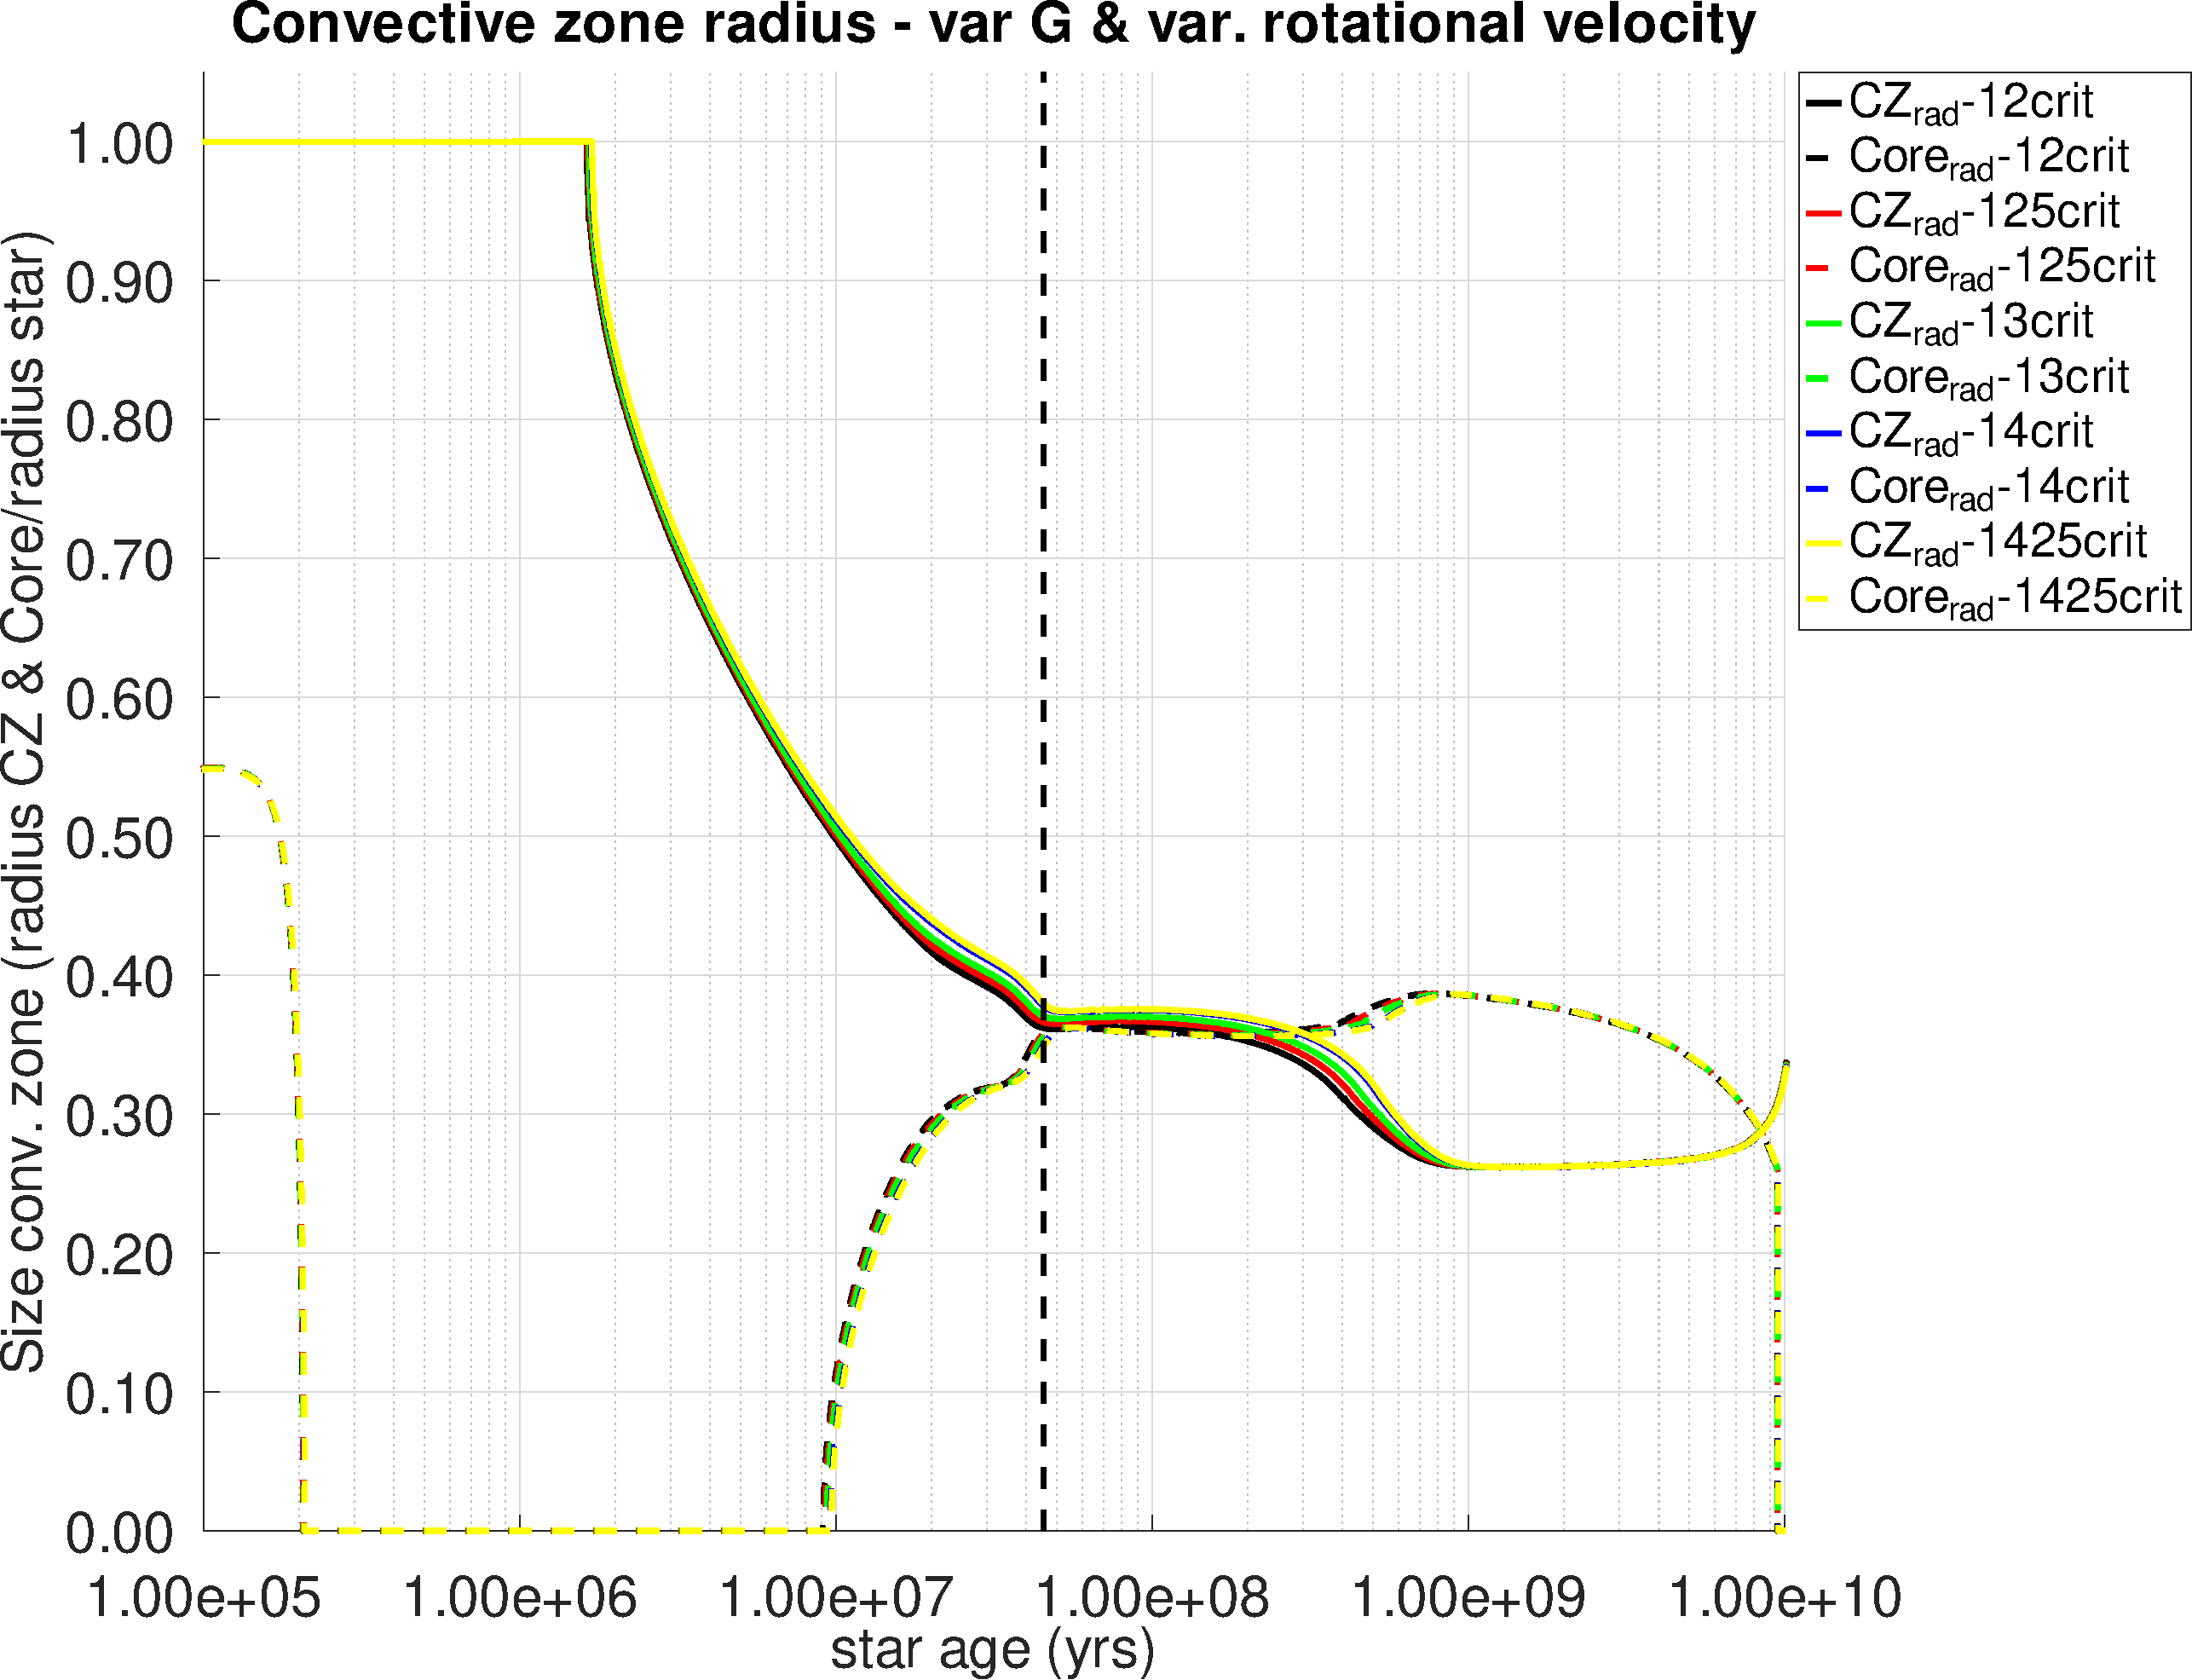
\includegraphics[clip,width=\columnwidth]{figures/paper2/cz_var_vel_var_g3.pdf}
    \caption{The evolution of the convective zone size as a function of time for several 1 $\msun$ models. The size is expressed in terms of $\rsun$. The models include a magnetic field with variable intensity, initial rotation with $\omegaini$ between 0.12 and 0.1425. The dashed vertical line makes reference to the ZAMS.}
    \label{fig:cz_var_vel_var_g3}
\end{figure}


The effects of rotation and magnetic braking can also be seen in the H-R diagram and in the evolution of the $\amlt$. The inclusion of rotation implies the appearance of centrifugal forces that affect both the structure of the star, the chemical composition of the different strata that compose it, as well as its temperature and luminosity. The differential rotation between the boundaries of the radiative core and the convective layers leads to mixing effects in the so-called tachocline. The outcomes of this mixing and its hydrostatic impacts are controlled by the MLT, where $\amlt$ assumes a crucial role. As previously stated, the arbitrariness of the $\amlt$ value introduces a level of uncertainty into the MLT. Figure \ref{fig:alpha_mlt_var_vel_g3} shows how the $\amlt$ parameter evolves over time.\par 

%The effects of this mixing and of its hydrostatic effects are governed by the MLT in which the $\amlt$ plays a major role in it. As aforementioned, MLT suffers from the arbitrariness of the value of $\amlt$.

\begin{figure}
	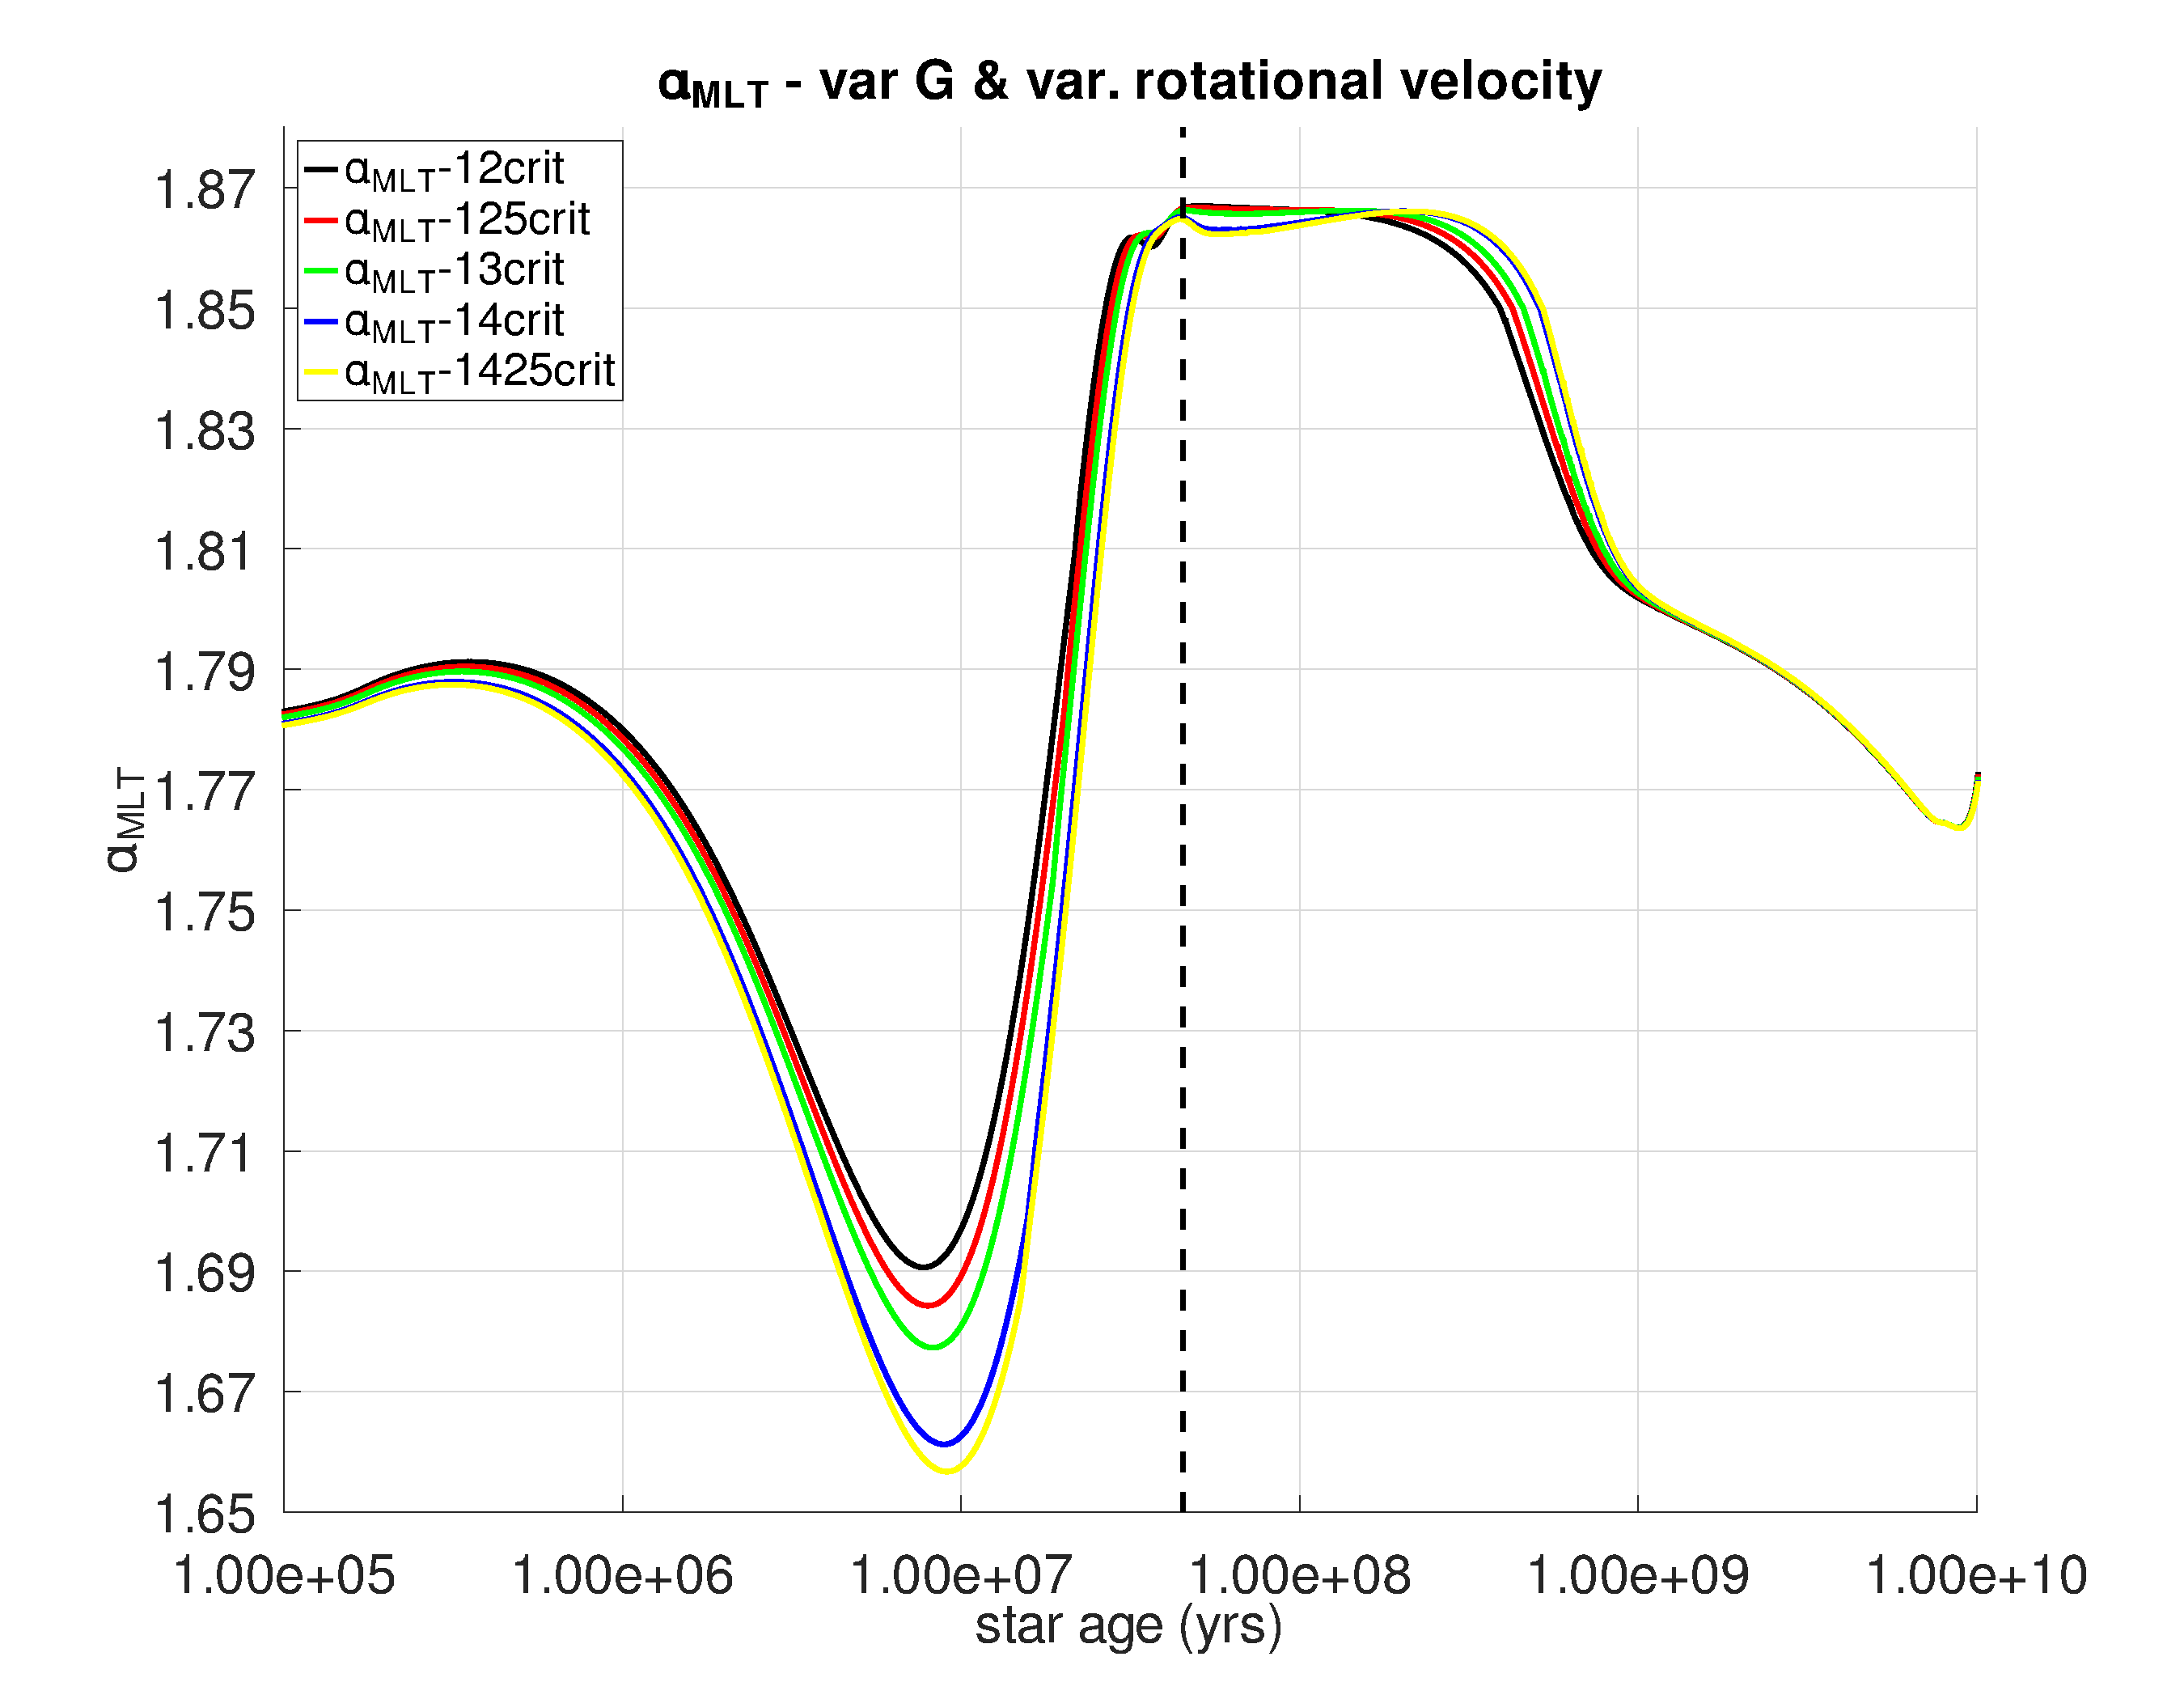
\includegraphics[clip,width=\columnwidth]{figures/paper2/alpha_mlt_var_vel_g3.pdf}
    \caption{The evolution of $\amlt$, as a function of time and $\omegaini$ for several 1 $\msun$ models. The models include initial rotation with $\omegaini$ between 0.12 and 0.1425. The dashed vertical line makes reference to the ZAMS. The purple star and diamond are the $\amlt$ given by \citet{Sonoi2018} and \citet{Samadi2005}, respectively.}
    \label{fig:alpha_mlt_var_vel_g3}
\end{figure}

Additionally, these same centrifugal forces, accentuated in stars with a higher angular velocity, reinforce the gravity darkening \citep[see e.g. ][]{Eggenberger2012,Paxton2019,Gossage2021} as well. The centrifugal force causes the star to shift its mass outward with respect to the rotation axis, the effect being more pronounced in the equatorial regions than at the poles. The consequence is that the pressure ($\gsurf$) to which the gas is subjected is lower in the former than in the latter. This effect causes stars that rotate fast enough to appear less dense ($\rho$), less luminous ($L$) and therefore with a lower effective temperature ($\teff$) as they approach the ZAMS (see Figure \ref{fig:hr_var_vel_var_g_z13}). If we compare the non-rotating model (black solid line in Figure \ref{fig:hr_var_vel_0g}) with the rotating ones, we can recognize that at the end of the PMS, the latter reach the ZAMS with a lower $\teff$ than the former. This also has an impact on the evolution of $\amlt$ because, as discussed above, in our model its value depends proportionally on $\teff$ and $\gsurf$. Both parameters are comparatively smaller for stars that rotate faster than for those that rotate more slowly. As a consequence $\amlt$ yields a lower value in its time evolution in those phases in which the star rotates faster, being this effect more accentuated in the ZAMS approach.\par

\begin{figure}
	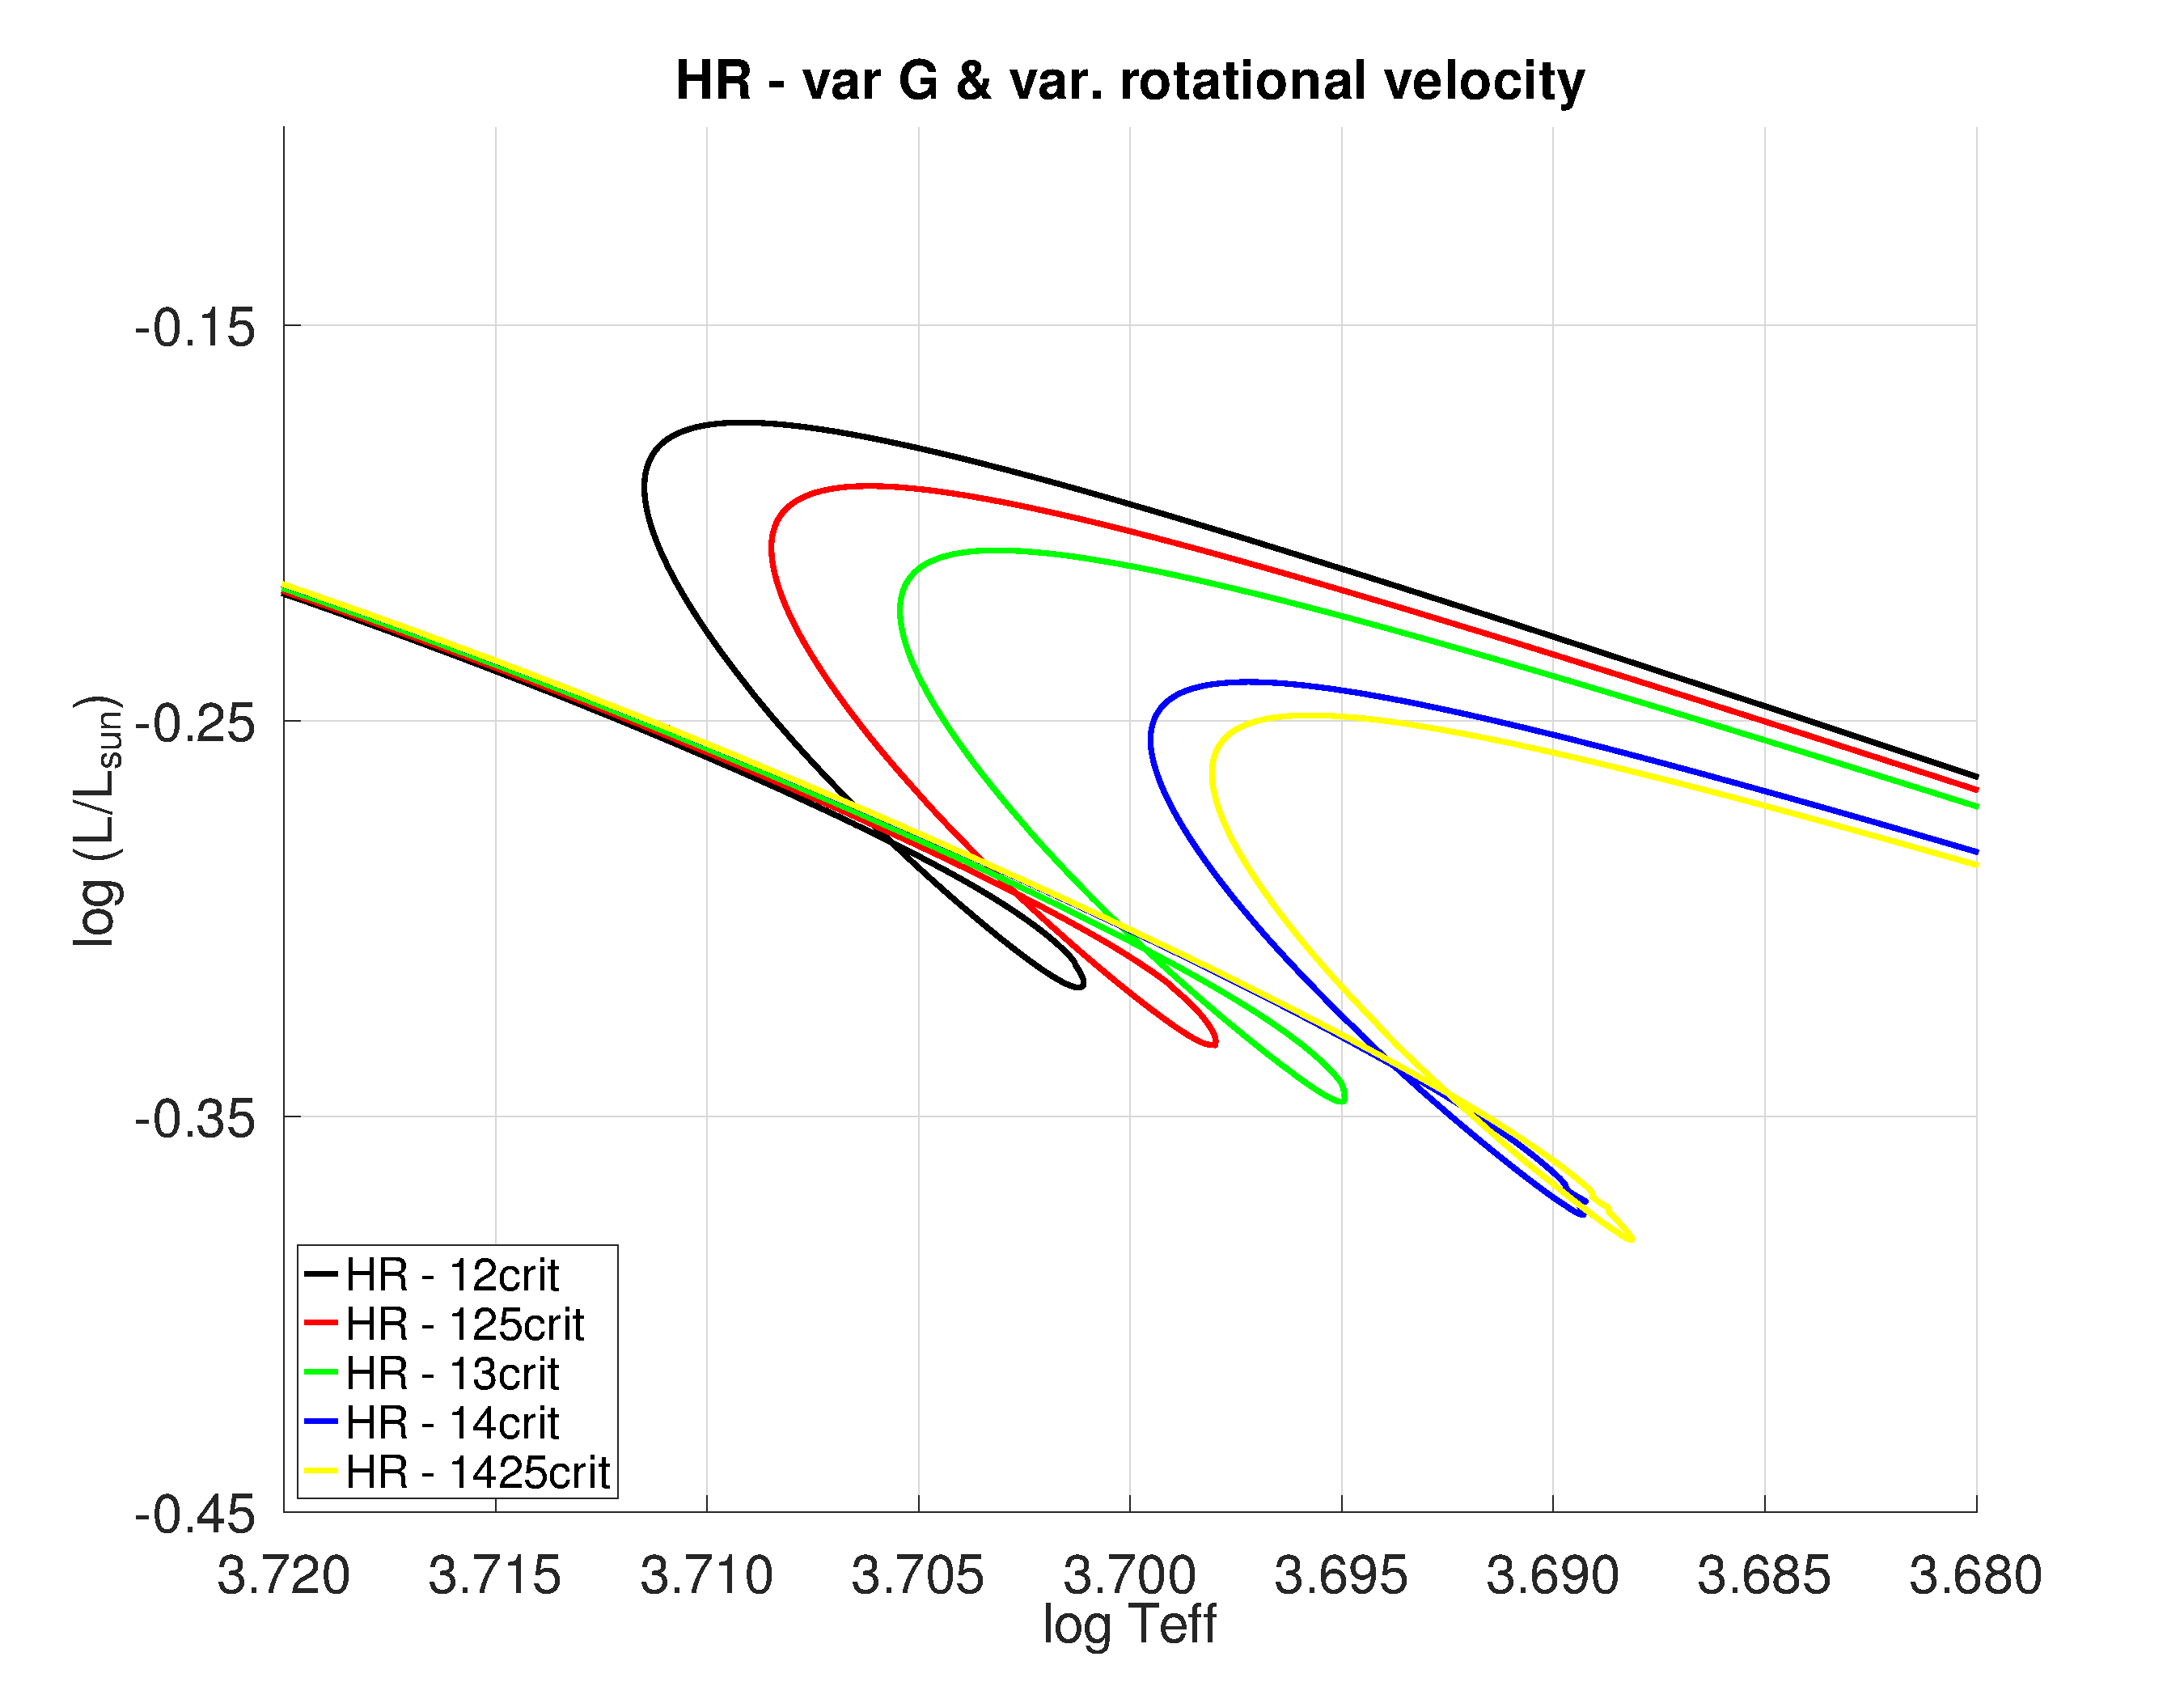
\includegraphics[clip,width=\columnwidth]{figures/paper2/hr_var_vel_var_g_z13.pdf}
    \caption{An example solar 1$\msun$ grid of stellar evolutionary tracks covering a range of angular velocities. It shows in detail the combined effects of the gravity darkening and magnetic braking on the evolutionary tracks. The models include a magnetic field with variable intensity, initial rotation with $\omegaini$ between 0.12 and 0.1425. The presence of a magnetic field produces hotter stars due to the influence of the magnetic braking on the rotational velocity of the star.}
    \label{fig:hr_var_vel_var_g_z13}
\end{figure}

\begin{figure}
	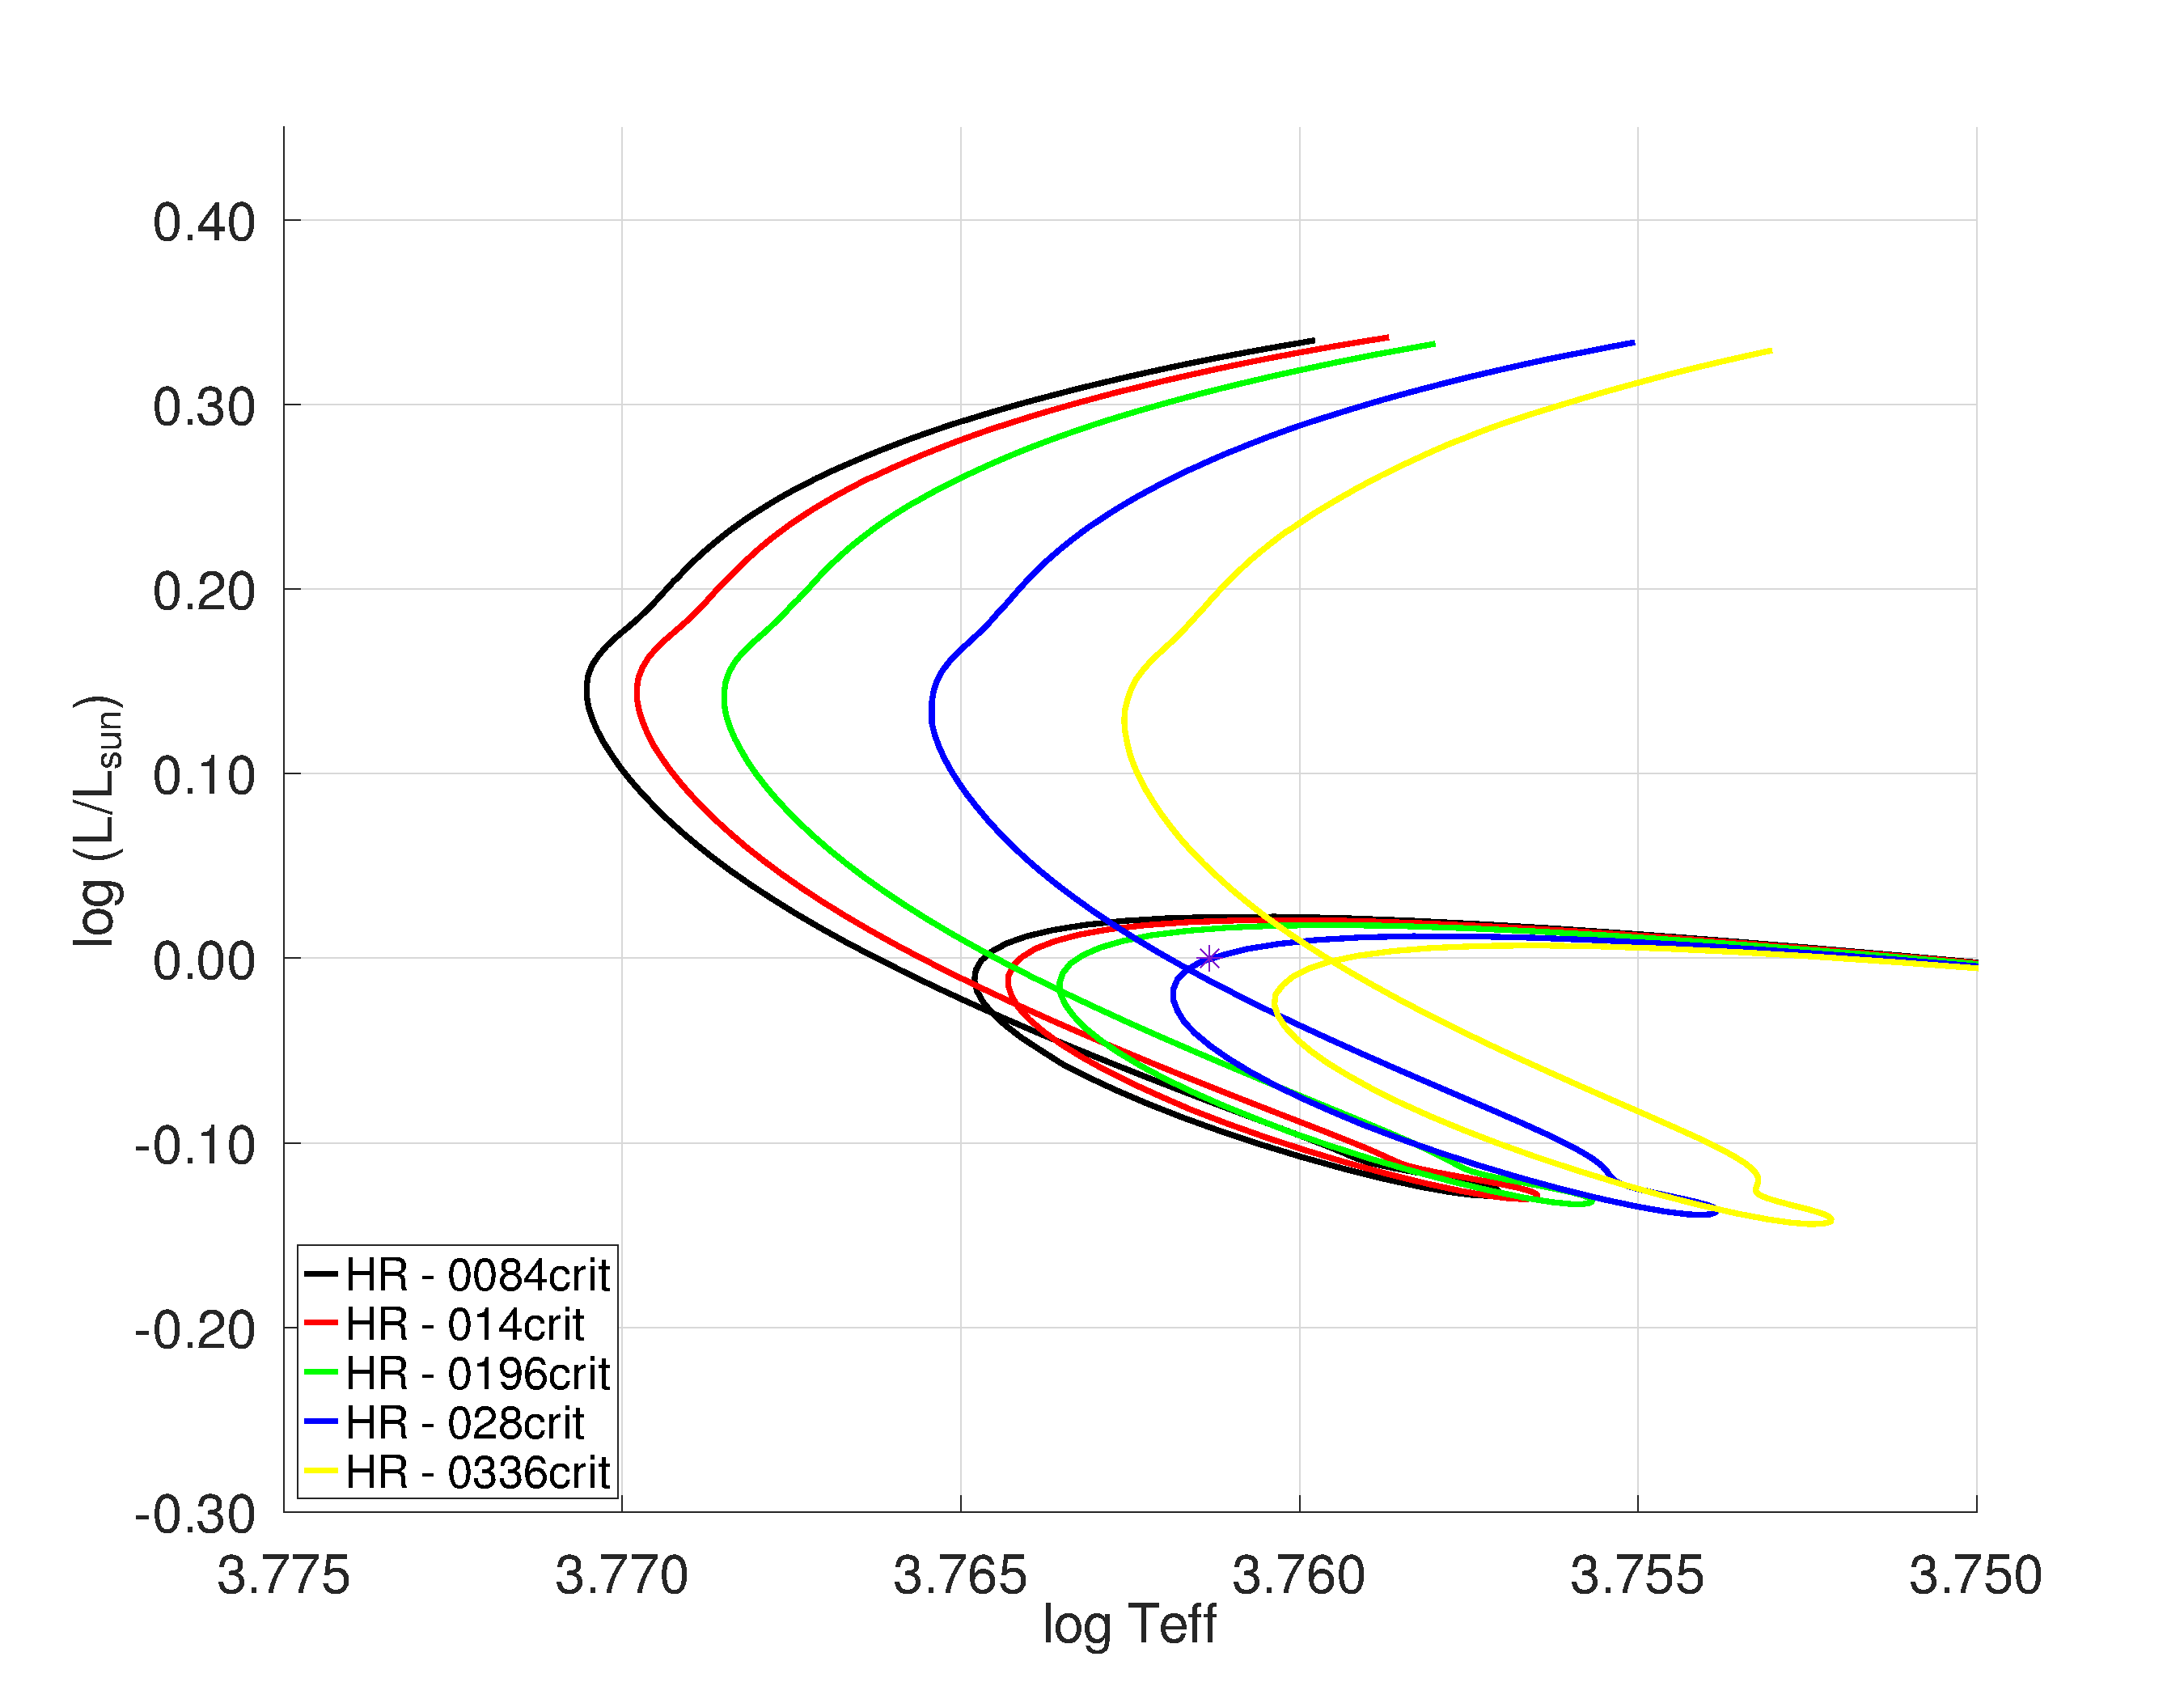
\includegraphics[trim = 10mm 10mm 15mm 10mm, clip,width=\columnwidth]{figures/paper2/hr_var_vel_0_0g_z10.pdf}
    \caption{Similar to Figure \ref{fig:hr_var_vel_var_g_z13} but now showing stellar evolutionary tracks in the absence (0G) of a magnetic field. The rotation is activated in the models in the PMS and those models reach before the ZAMS and at a lower $\teff$ than the non-rotating one (solid black line). The luminosity is expressed in terms of $\lsun$. $\lsun$ = 3.761. (Figure taken from \citet{Caballero2020}.)}
    \label{fig:hr_var_vel_0g}
\end{figure}

Figure \ref{fig:teff_logg_var_vel_g3} shows how $\teff$ and $\gsurf$ behave over the evolution of the models. For those with a higher rotation speed, we observe that both their temperature and surface gravity are lower than in the slower rotating models, in line with the gravity darkening. It is worth noting that in the ZAMS approach phase we observe for the fastest rotating model (yellow) that its surface gravity is higher than that of the rest of the slower models. This can be explained by looking at Figure \ref{fig:lograd_var_vel_g3}, which shows the evolution of the stellar radius for the different models, as a function of time and $\omegaini$. Around the interval $2.5x10^{7}$ and $3.5x10^{7}$ Ga (delimited by the cyan lines) and after the ZAMS, from around $5.4x10^{7}$ to $11.2x10^{7}$ Ga (delimited by the magenta lines) the stellar radius of the fastest model is smaller than that of the rest, producing a higher $\gsurf$, and this in turn means less mass loss (see Fig. \ref{fig:mdot_var_vel_g3}). During this period the fastest model does so at a lower rate and expose a higher surface gravity. Let us recall that the stellar radius has an inversely quadratic influence on the value of $\gsurf$. This "anomaly" disappears as soon as the stellar radius becomes again bigger for the fastest model.\par


\begin{figure}
	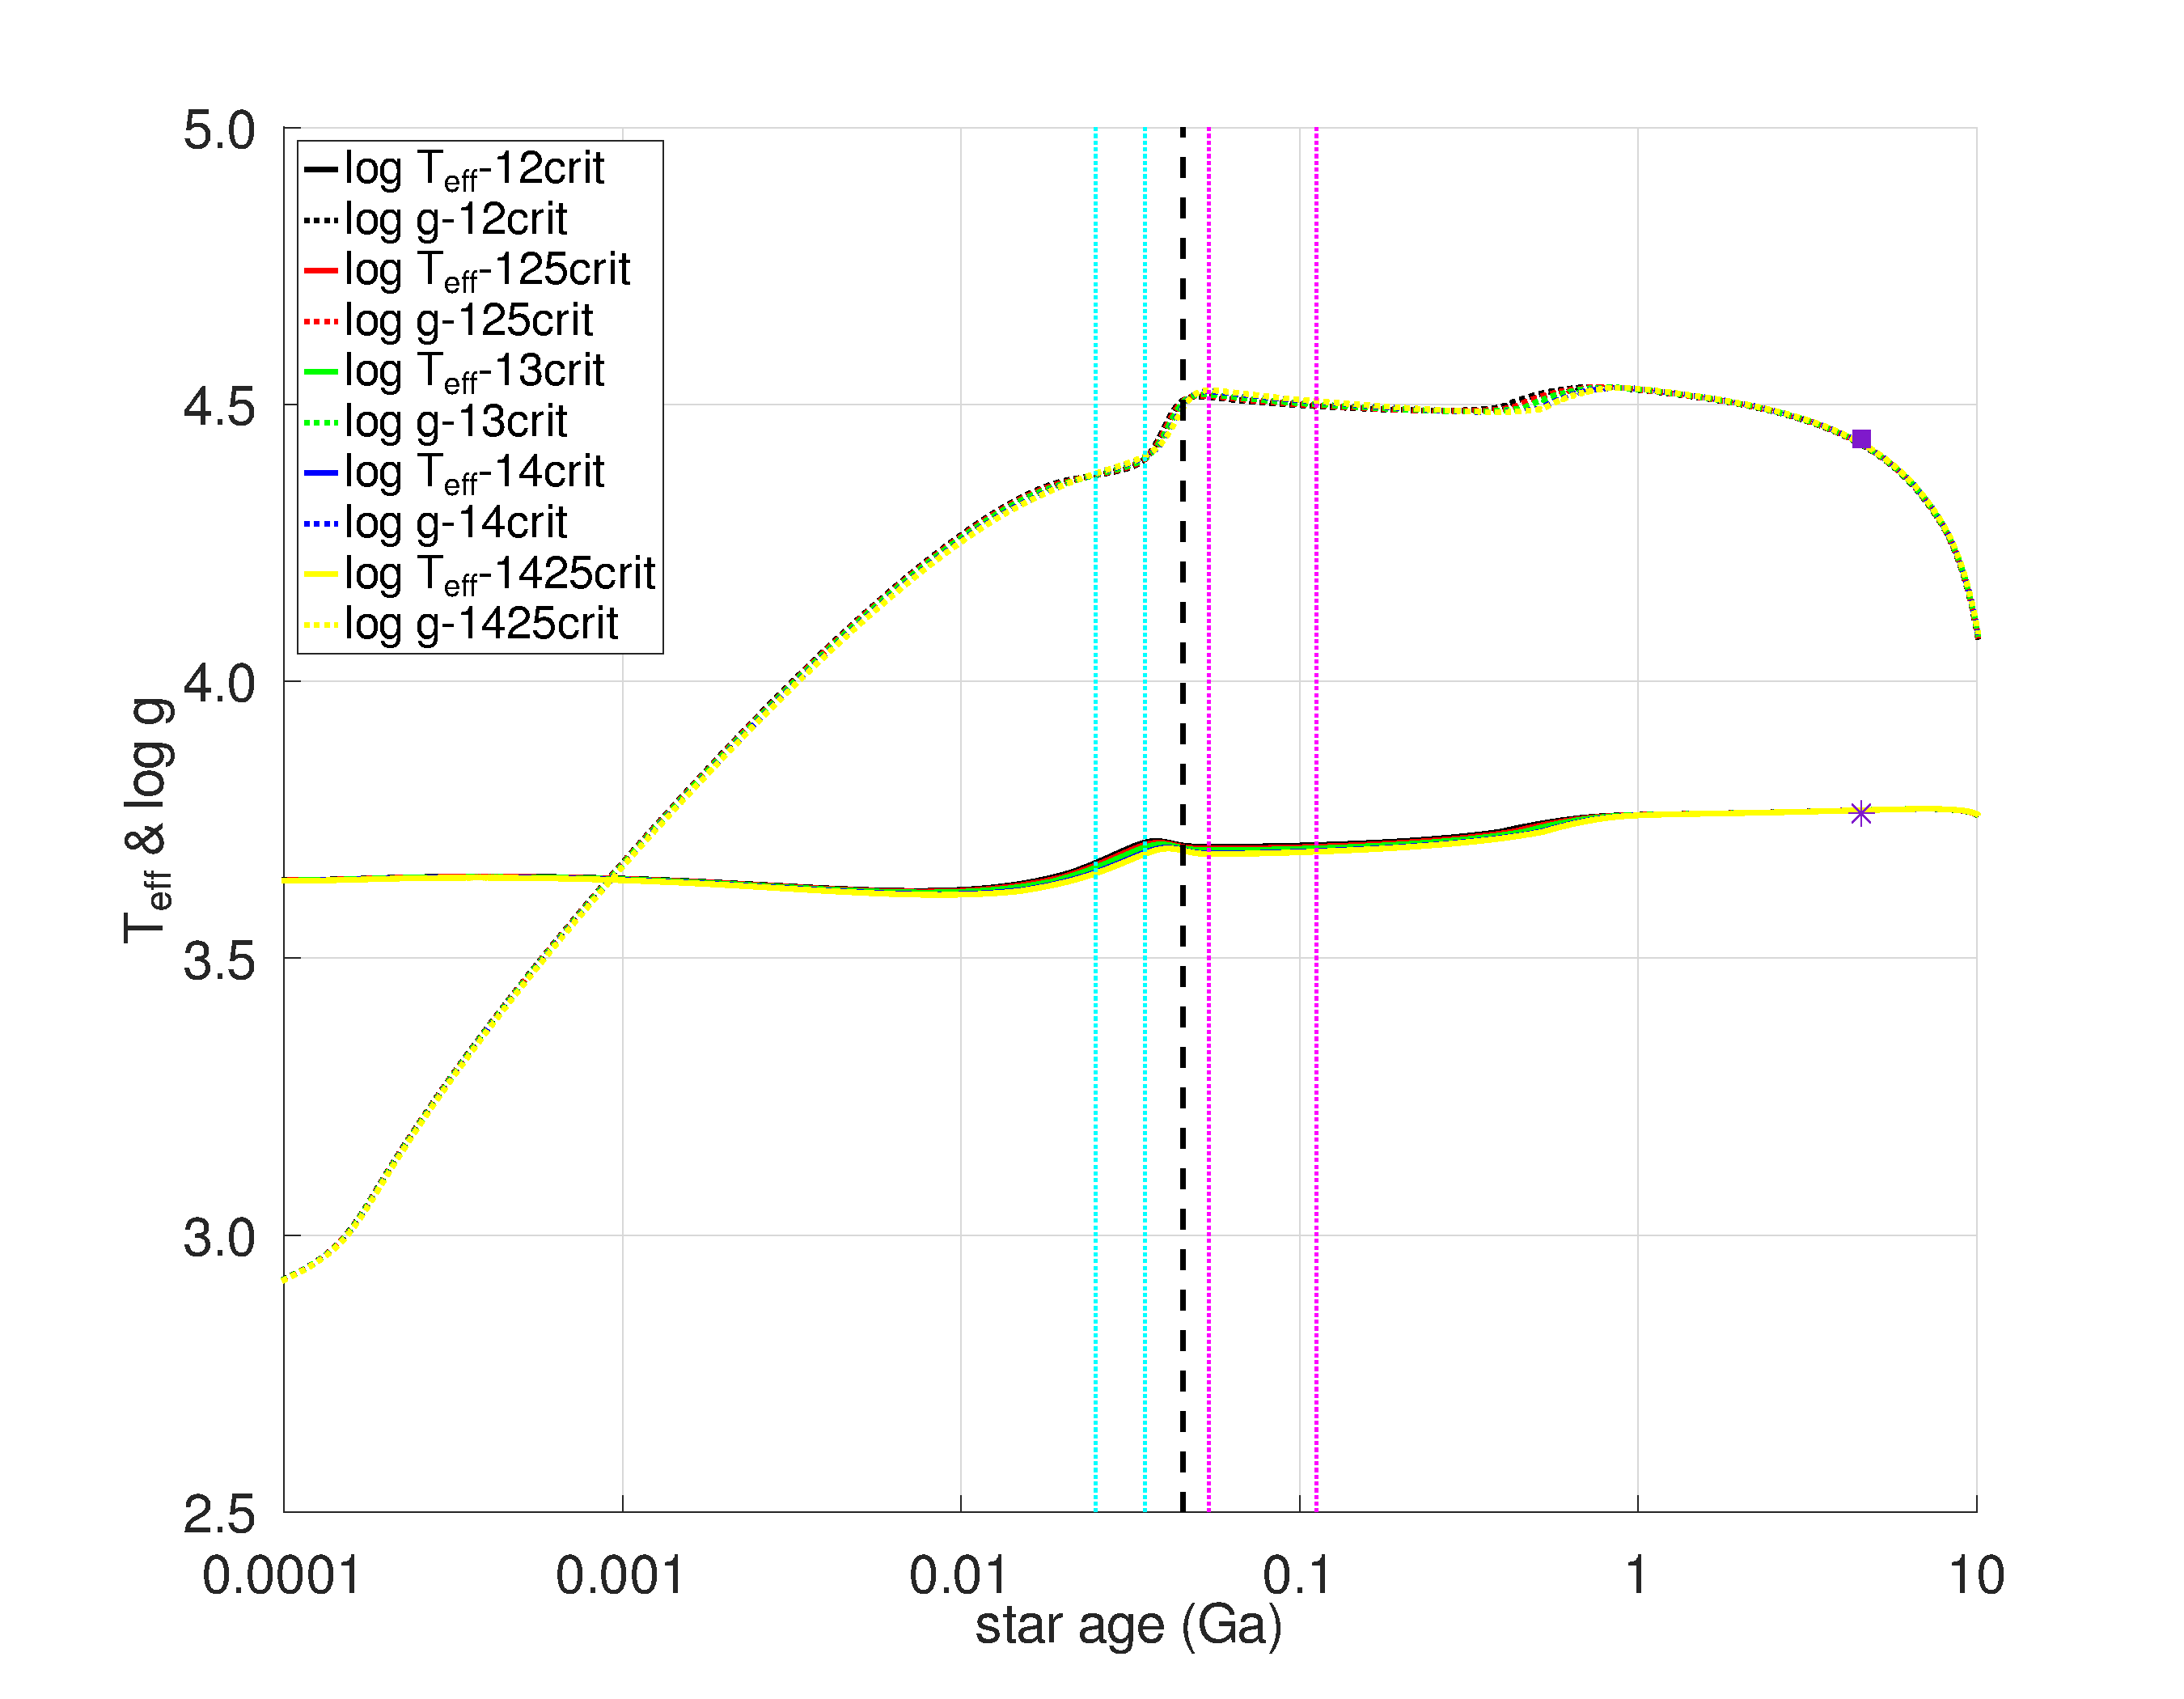
\includegraphics[clip,width=\columnwidth]{figures/paper2/teff_logg_var_vel_g3.pdf}
    \caption{The evolution of $\teff$ and $\gsurf$, as a function of time and $\omegaini$ for several 1 $\msun$ models. The models include initial rotation with $\omegaini$ between 0.12 and 0.1425. The age intervals [$2.5x10^{7},3.5x10^{7}$] Ga and [$5.4x10^{7},11.2x10^{7}$] Ga, delimited by the cyan and magenta lines respectively, highlight periods in which the fastest model with $\omegaini$=0.1425 exposes a surface gravity higher than that of the rest of the slower ones. The purple star is the $\teff$, and the purple square is the $\gsurf$ for the present-day Sun \citep{Gill2012}. The dashed vertical line makes reference to the ZAMS.}
    \label{fig:teff_logg_var_vel_g3}
\end{figure}

\begin{figure}
	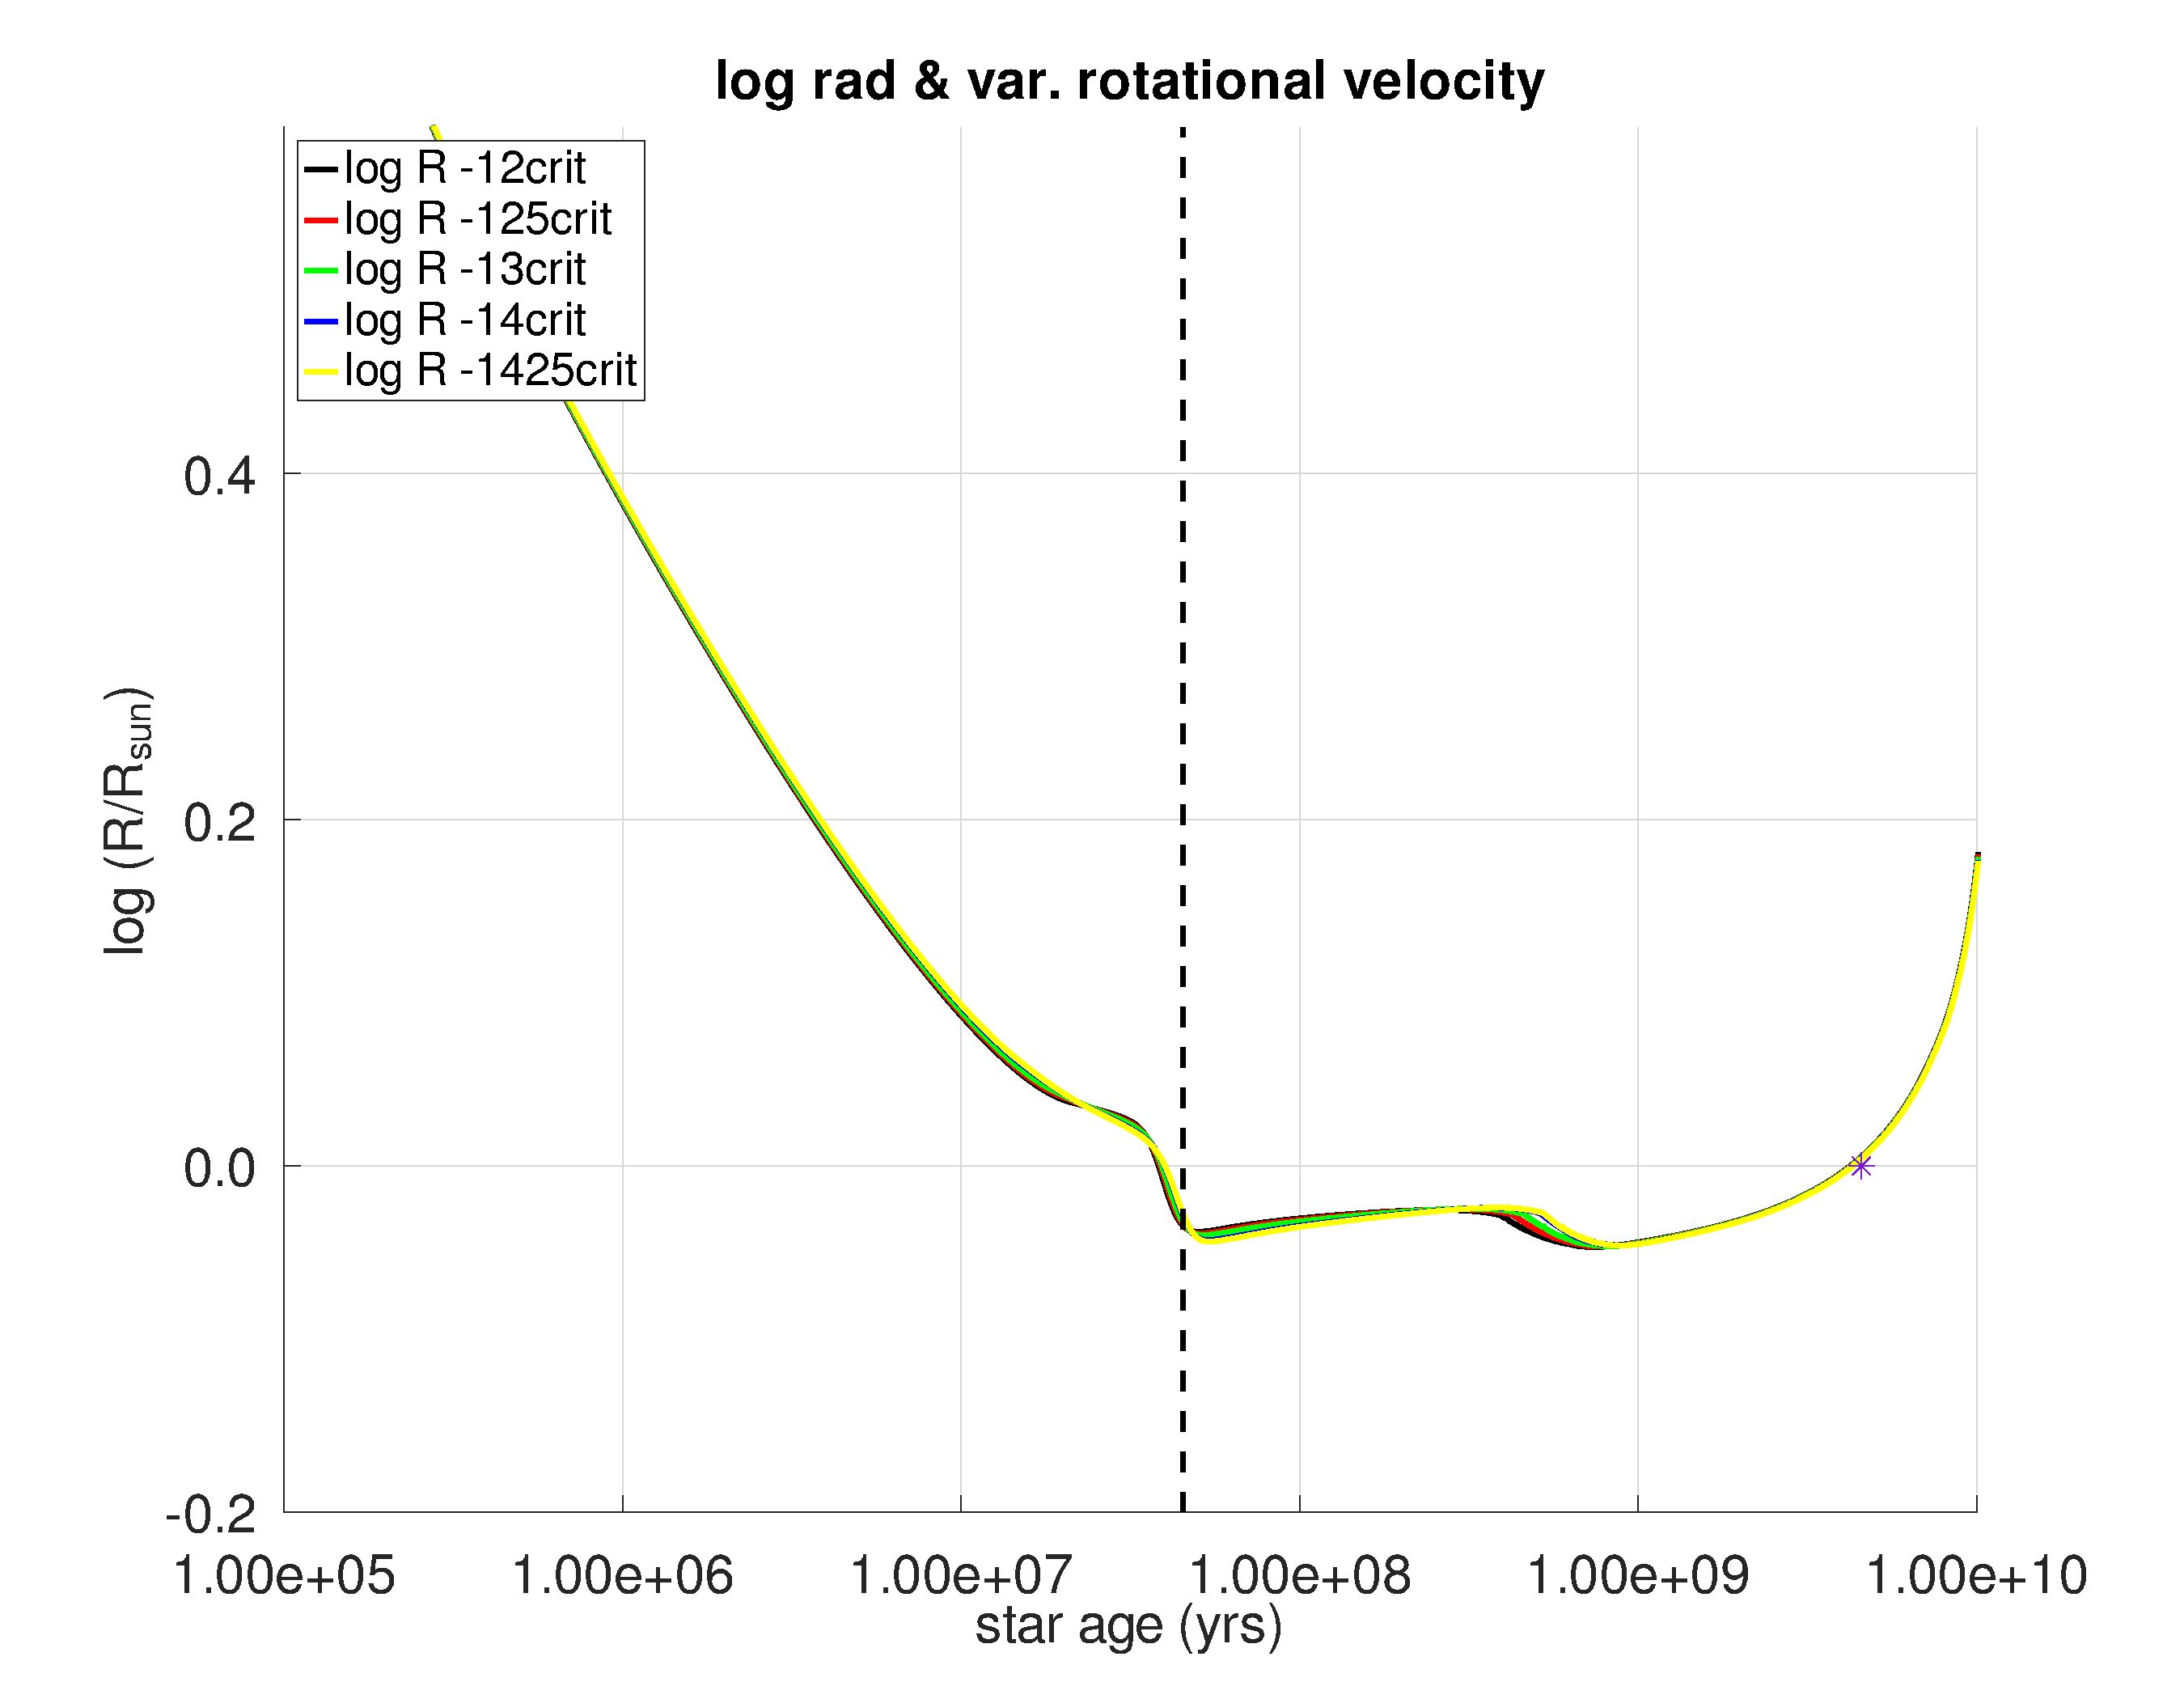
\includegraphics[clip,width=\columnwidth]{figures/paper2/lograd_var_vel_g3.pdf}
    \caption{The evolution of the stellar radius, as a function of time and $\omegaini$ for several 1 $\msun$ models and their. The models include initial rotation with $\omegaini$ between 0.12 and 0.1425. The purple star is the radius for the present-day Sun \citep{Gill2012}. The dashed vertical line makes reference to the ZAMS.}
    \label{fig:lograd_var_vel_g3}
\end{figure}

\subsection{Caballero et al. (2020) Comparison}
In \citet{Caballero2020} we have already addressed the study of the lithium surface abundance in the Sun. That previous work laid the foundations for the development of the present. In it, we advanced as future lines of research a deeper understanding about how magnetic fields are linked to rotation and how they evolve in time. We also showed how by adjusting the value of $\amlt$ we were able to influence the in the Li abundances. Therefore, a comparison between the results obtained previously and those of this study puts into perspective the differences and similarities between the two studies, as well as the advances made since then. The Table \ref{tab:caballero2023_2020} summarises the main differences between the two works, in line with what is already advanced i.e. we incorporate formalisms that allow us to temporally evolve the $B$ and $\amlt$.\par 

\begin{table}
	\centering
    \begin{threeparttable}
	\begin{tabular}{lll} 
		\hline
		Parameter & This work & \citet{Caballero2020}\\
		\hline
		Convection & MLT variable $\alpha_{{\rm MLT}}$ & MLT fixed $\alpha_{{\rm MLT}}=1.82$\\
            Overshoot & deactivated & $f_{{\rm ov,core}}=0.0160$,\\ & & $f_{{\rm ov,sh}}=0.0174$\\
		Magnetic Braking & \citet{Gallet2013} & \citet{Ud-Doula2008} \\ Formalism & & \\
		Magnetic Field & B(G) variable & B(G) pre-set [3.0G-5.0G]\\ Strength & & \\
            Number of OC's & 64 & 1 \\
            Source of data & GDR3.0 GES DR5.0 & \citet{Sestito2005} \\
		\hline
	\end{tabular}
    \end{threeparttable}
    \caption{Comparison with \citet{Caballero2020} work.} \label{tab:caballero2023_2020}
\end{table}

The Figure \ref{fig:li_var_vel_4_0g4} shows the evolution of Li abundance for $\omegaini$ between 0.0084 and 0.0336 in the presence of a magnetic field with an intensity of 4G. We have augmented the original version with the same set of OCs data gathered applied in this new work, so that a consistent comparison between both formalism is possible. If we focus our attention on the simulation with $\omegaini$ = 0.0336, the simulation reproduces  A(Li) = 1.024 dex, a value which is in line with both that of the Sun (1.1 $\pm$ 0.1 dex) and the values obtained in Figure \ref{fig:li_var_vel_var_g_3} for the present work (1.133 dex) for $\omegaini$ = 0.14 and 0.1425. Although in the latter case the models were initialized at higher $\omegaini$ values than in the former, resulting in $B$ up to 3 orders of magnitude more intensive ($\approx$ 1KG versus 4G) the simulation in both works end up in producing very similar values for both the rotational velocity and the A(Li). This is partially explained because a higher magnetic field strength implies an intensive MB effect (refer to Figures \ref{fig:rot_vel_var_vel_var_g3} \& \ref{fig:rot_vel_var_vel_4_0g4}). In the former case, the deceleration effect is sharper than in the latter, so it ceases to destroy Li before.\par

However, this effect is not sufficient to effectively counteract the destruction of Li. The other decisive element that comes into play is the value of $\amlt$. As exemplified in \citet{Caballero2020} its value has an inversely proportional impact on Li destruction, where a lower value resulted in less Li destruction, particularly during PMS. In the figure \ref{fig:alpha_mlt_var_vel_g3} we observed the temporal $\amlt$ value evolution. Until the latest phase of the PMS, the value $\amlt$ is substantially less than 1.82, the pre-set and invariant value used in our previous work, resulting in less Li destruction and allowing the model to reach the ZAMS with a $\approx$ 29\% dex higher Li reservoir. This major Li reserve compensates for the greater destruction induced by the models initialized with a $\omegaini$ higher angular velocity.\par

Similarly, we proceed to show the evolution of the surface rotational velocity in Figure \ref{fig:rot_vel_var_vel_4_0g4} and select the simulation with $\omegaini$ = 0.0336. Again, the similar values are explained by the higher efficiency of the MB in the new model. Although the simulations reach the ZAMS with rotational velocity values up to 200\% for the models initialised with higher $\omegaini$, the stronger magnetic field produces a more pronounced deceleration for the same time interval. This fact is especially noticeable in the time period between the ZAMS and 1 Ga. The rotational velocity obtained at the equator of 4.82 km/s is a value quite close to 4.72 km/s, that is, the value simulated for $\omegaini$ = 0.0336 (Fig.~\ref{fig:rot_vel_var_vel_var_g3}).\par

In view of the values obtained, we can draw the conclusion that the new model introduced in the current work is not only congruent with the results of the works on which it is based, but also with those of \citet{Caballero2020}. Additionally, this new version exposes the advantage of not having to resort to the use of preset values for $B$ and $\amlt$, and without recurring to activate the overshooting. All in all, this represents a significant improvement and supports our line of research aimed to avoid preset values by making them to evolve dynamically with key solar parameters.\par


\begin{figure}
	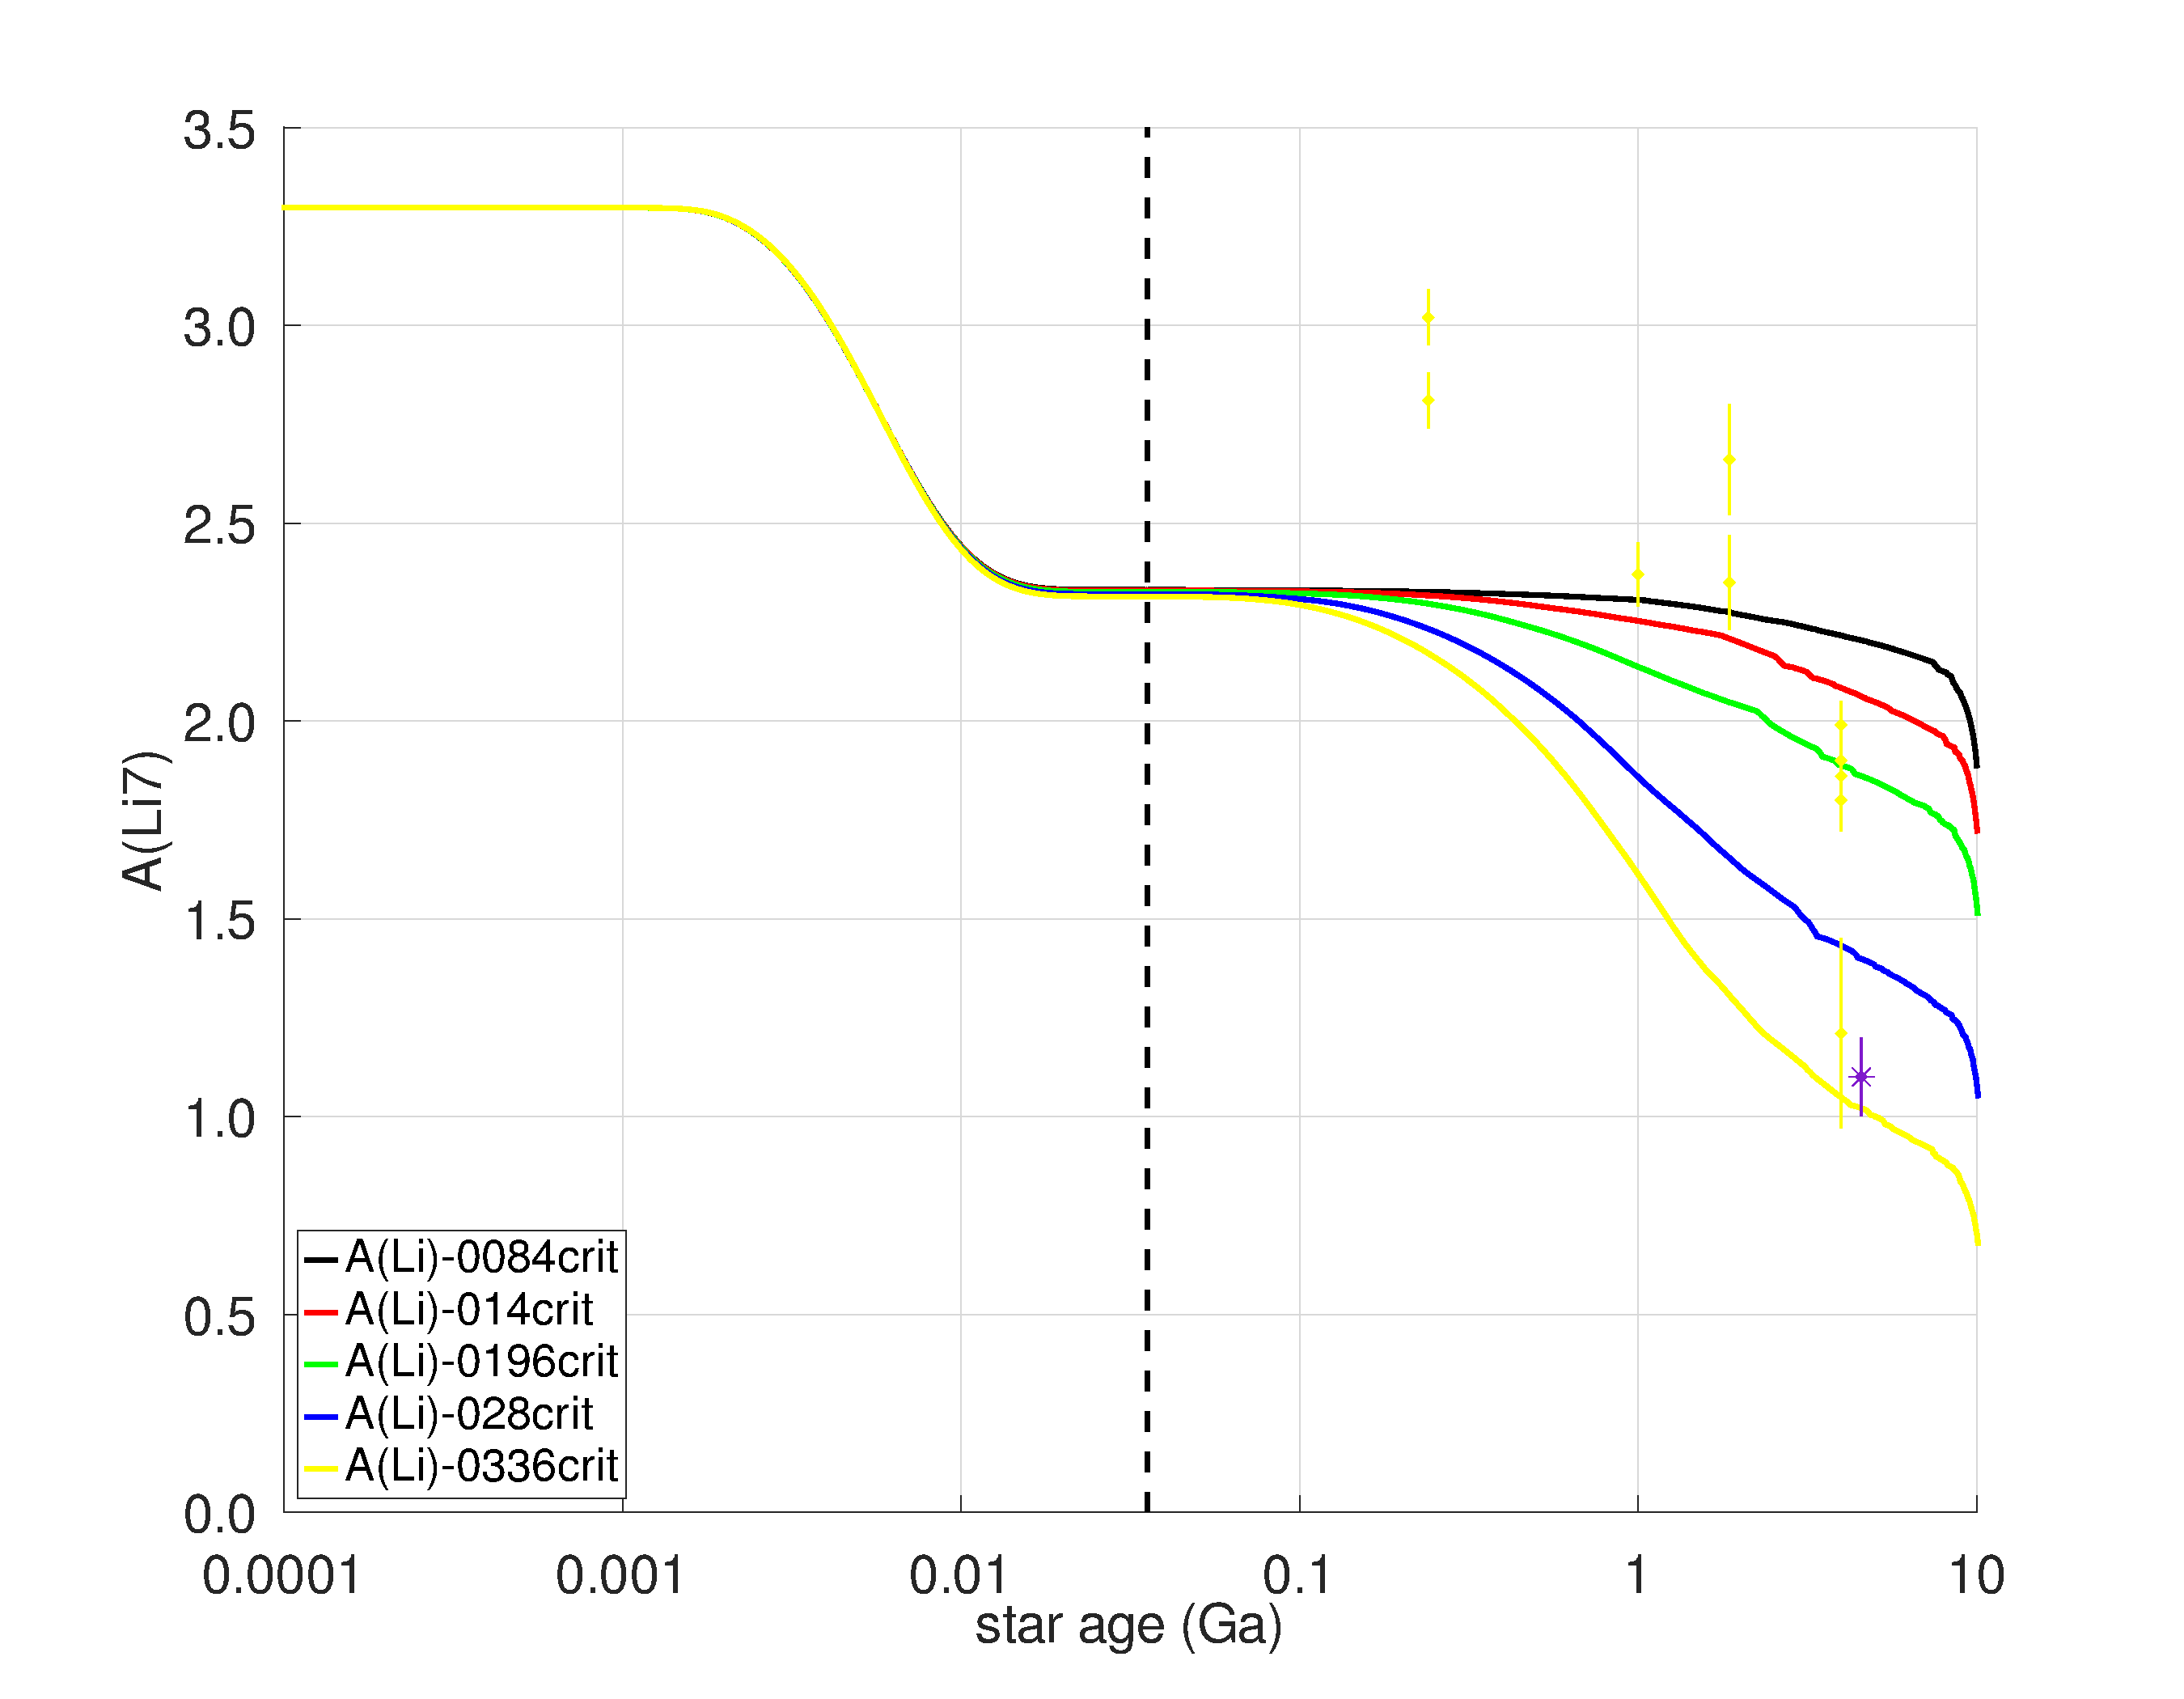
\includegraphics[clip, width=\columnwidth]{figures/paper2/li_var_vel_4_0g4.pdf}
    \caption{The evolution of surface \isotope[7]{Li} abundance relative to \isotope[1]{H}, as a function of time for several 1 $\msun$ models. The models include a magnetic field with an intensity of 4G. The solid black line represents the reference model according to \citet{Choi2016}. The rest of lines are models which include initial rotation with $\omegaini$ between 0.0084 and 0.0336, respectively. The purple star is the surface Li abundances for the present-day Sun \citep{Asplund2009}. The dashed vertical line makes reference to the ZAMS.}
    \label{fig:li_var_vel_4_0g4}
\end{figure}

\begin{figure}
	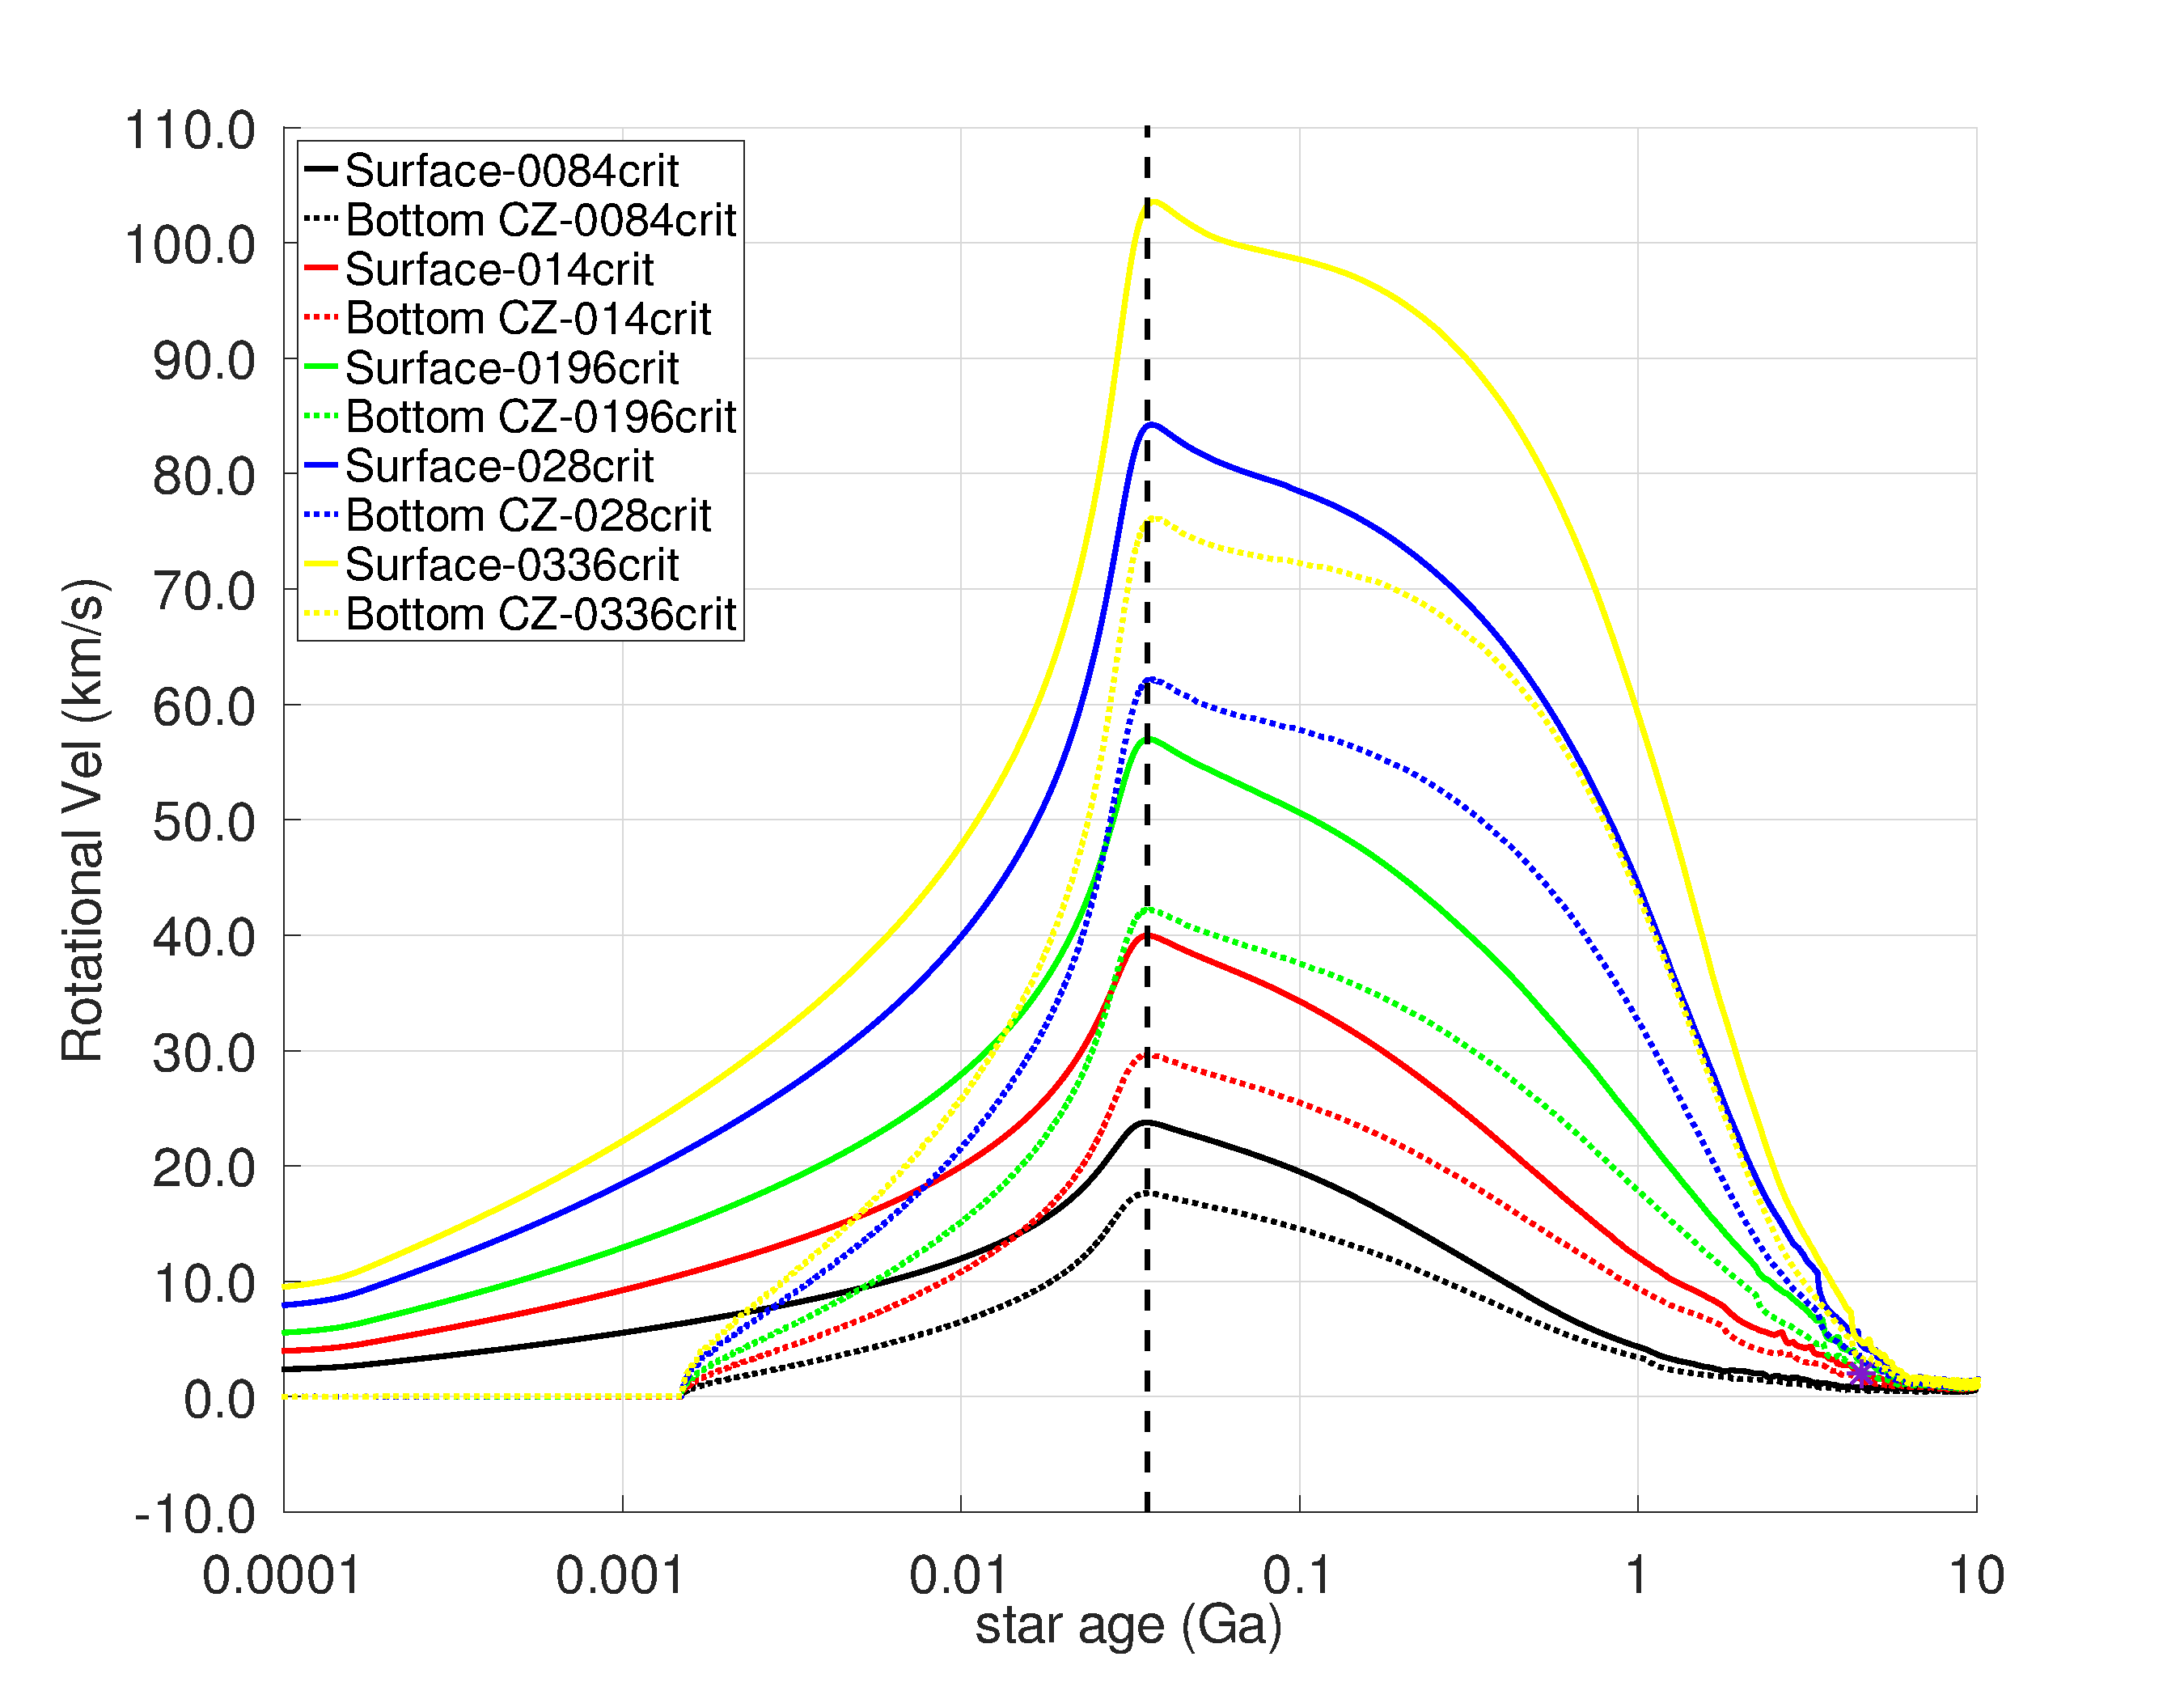
\includegraphics[clip,width=\columnwidth]{figures/paper2/rot_vel_var_vel_4_0g4.pdf}
    \caption{The evolution of surface rotational velocity, as a function of time for several 1 $\msun$ models. The models include a magnetic field with an intensity of 4G, initial rotation with $\omegaini$ between 0.0084 and 0.0336, respectively and MB. The purple star is the surface angular velocity for the present-day Sun \citep{Gill2012}. The dashed vertical line makes reference to the ZAMS.}
    \label{fig:rot_vel_var_vel_4_0g4}
\end{figure}



\subsection{Gossage et al. (2021) Comparison}
Due to the existence of similarities between \citet{Gossage2021} work and this one, we proceed to make a comparison between the two of them. Among the similarities we find the fact that both papers focus on magnetic braking, making use of MESA for the simulations. Among the main differences is that our models incorporate a variable $B$ and $\amlt$. Finally, both compare their simulation results (rotation periods and Li abundances) with starts located in OCs.\par

In \citet{Gossage2021}, the authors also approach the problem of AML from a similar starting point to ours, but with some notable variations. In the Table \ref{tab:gassage_vs_navarro} we compare the similarities and differences between the two studies. In both works the models consider rotation not only in the MS but also in the PMS, with the distinction that in Gossage's work they take into account disk-locking. This aspect is not so relevant in our simulations since we have focused on the A(Li) profiles, and Gossage's work focuses mainly on modeling rotation profiles of stars, which are significantly impacted by the disk-locking mechanism. Similarly, the effects of magnetic braking on angular momentum loss are also considered, in our case for stars with 1$\msun$ (solar twins) and in their with 0.1$\msun$$\le$$\mstar$$\le$1.3$\msun$. Both models also use MLT but in our case the value $\amlt$ is not prefixed but varies throughout the simulation.\par

These two works complement each other as they are based on different formalisms. On the one hand, our work is based on the proposal of \citet{Gallet2013} whose most relevant parameters are $\rossby$ and the presence of a magnetic field of varying strength (B), whereas Gossage presents two formalisms: \citet{Matt2015} and \citet{Garraffo2018}. The former is mainly characterised by $\rossby$ and the $\mstar$, while the latter by $\rossby$ and a parameter that accounts for the complexity of the magnetic fields, being equal to 1 for a dipole field and larger for higher-order multipoles. As far as OCs observations are concerned, here we covered a wider range of ages [0.001-6.761] Ga. Finally, both papers simulate their respective models in MESA but use different versions.\par

\citet{Gossage2021} manage to reproduce more accurately the Sun's rotation profile at its current age \citep[see][panel (a) in Figures 2, 4 \& 6]{Gossage2021} although, as the authors of the paper describe, they calibrated their models to do so, by including an additional diffusion-free parameter ($v_0$). In our work, our model does not include this type of additional parameterization and is still able to reproduce an equatorial rotation speed of 4.72 km/s, a value not particularly far from the nominal set value of 2.0 km/s. As far as A(Li) is concerned, their model does not reproduce the value for Sun-like stars, including the Sun itself \citep[see][panel (d) in Figures 2 \& 4, and (b) in Figure 6]{Gossage2021}. By recalibrating some of the parameters of their model and/or incorporating additional mechanisms that contribute to Li destruction, the authors hope to obtain values in line with observational data. In our case (see Section \ref{sec_conclusions}), we were able to reproduce A(Li) with greater precision.

\begin{table}
	\centering
    \begin{threeparttable}
	\begin{tabular}{lll} 
		\hline
		Parameter & This work & \citet{Gossage2021}\\
		\hline
            
		Rotation & At PMS \& MS & At PMS \& MS\\
  		Solar Mass & $\mstar$=1$\msun$ & 0.1$\msun$$\le$$\mstar$$\le$1.3$\msun$ \\
		Convection & MLT variable $\alpha_{{\rm MLT}}$ & MLT fixed $\alpha_{{\rm MLT}}$\\
		Magnetic Braking & \citet{Gallet2013} & \citet{Matt2015}, \\ Formalism & & \citet{Garraffo2018}\\
		Magnetic Field & B(G) variable & B(G) pre-set\\ Strength & & \\
            Disk locking & Not present & Present\\
            Number of OC's & 64 & 11 \\
            Source of data & GDR3.0 GES DR5.0 & Several works \\
            MESA version & r10398 & r11701\\
		\hline
	\end{tabular}
    \end{threeparttable}
	\caption{Comparison with \citet{Gossage2021} work.}\label{tab:gassage_vs_navarro}    
\end{table}


\section{Conclusions and future works} \label{sec_conclusions}
Through various simulated stellar models, we've demonstrated that the interplay of rotation and magnetic braking can align observational data with theoretical models, potentially through an $\Omega$-$B$ interdependence law. These models, unlike our previous ones, don't preset initial values for magnetic field strength and the $\amlt$ parameter. We've validated these models with Gaia and GES data for Sun-like stars, especially their Li abundances.\par

Our models suggest a lower Li abundance limit of 1.133 dex for Sun-like stars, within the Sun's error margin (1.1 $\pm$ 0.1 dex). They predict a higher equatorial rotational velocity (4.72 km/s) than the Sun (2.0 km/s), enabling more Li burning. Despite developing strong magnetic fields and intensive magnetic braking, our models don't match the Sun's omega value and average magnetic field strength.\par

While our evolving magnetic field strength and MLT parametrization align with observations, we must interpret these results cautiously. Key findings include:
\begin{enumerate}
    \item Varying magnetic field intensity is a valid alternative to preset models, aligning with previous work on Sun-like stars' rotational history.
    \item A variable adaptive $\amlt$ formalism eliminates the need for preset values, reproducing values consistent with previous work and providing potential value ranges when upfront $\amlt$ values are unknown or undesirable.
    \item Our models suggest a lower limit for A(Li)=1.133 dex to the Gaia and GES observations for solar twin stars.
    \item Despite initializing models at higher $\omegaini$ values than in our previous work, resulting in $B$ up to 3 orders of magnitude more intensive, $\approx$ 1KG versus 4G, both works' simulations produce similar values for rotational velocity and A(Li).
\end{enumerate}

In conclusion, enhancing our understanding of stellar interiors and Li depletion mechanisms for solar twins is crucial for more accurate comparisons. Broadening our models' mass range will enable us to compare results with a wider observational range. Our models currently over-deplete Li compared to Gaia and GES data.\par

Considering that faster rotating stars deplete more Li, additional mechanisms, like disk locking to the protostellar disk, are needed to explain observations. This introduces two braking mechanisms acting at different star ages, establishing a self-regulating mechanism influencing Li evolution and magnetic field strength, which could align with the Sun's lower intensities.\par

Lower rotational velocity means less Li destruction in our models. To compensate for this, we could use overshooting, an effect not simulated in our models, which would allow Li to be reached by hot material bubbles, decreasing its abundance. Ideally, like $\amlt$, overshooting should depend on other fundamental stellar parameters.\par


%We have shown, through the different simulated stellar models, that the effects induced by the combination of both rotation and magnetic braking mechanisms offer a plausible way to reconcile the observational data with the theoretical models. We propose that this result could be achieved by a law of interdependence between $\Omega$ and $B$. In contrast to our previous work, these new models remove the restrictions of pre-setting initial and fixed values along their time evolution for the magnetic field strength and the $\amlt$ parameter. We have cross-checked the model results with measurements obtained from the Gaia and GES mission for stars with similar characteristics to our Sun, focusing on their Li abundances.\par

%Our models seem to suggest a lower limit to the surface Li abundances of 1.133 dex for Sun-like stars, value which is within the margin of error obtained for the Sun (1.1 $\pm$ 0.1 dex). On the other hand, they predict a higher rotational velocity at equator (4.72 km/s) than the Sun (2.0 km/s) so that they could burn more Li and finally reproduced the Sun Li existing reservoirs. Coupled with this higher angular velocity, strong magnetic fields developed, triggering an intensive magnetic braking that slowed its angular velocity but not enough to match the present $\Omega$ value of the Sun. In addition, it should be noted that our models fail to replicate the average magnetic field strength of the Sun.\par

%Although we have shown how both an evolving magnetic field strength and, a MLT parametrization could produce results in line with the observations, we must analyse the results obtained with caution and not draw any premature conclusions. In spite of these shortcomings, we can draw the following finding from the present work:

%\begin{enumerate}
%    \item A magnetic field with varying intensity is a valid alternative to the models with a pre-fixed value as they produce results in line with previous work for the rotational history of Sun-like stars.
%    \item A variable adaptive $\amlt$ formalism could eliminate the need to prefix its value. By using it, we were able to reproduce values in line with previous works. Additionally, it could also serve to derive an interval of potential values in cases when an upfront $\amlt$ value is unknown or even not desirable.
%    \item Our models seem to suggest a lower limit for A(Li)=1.133 dex to the observations provided by Gaia and GES for solar twin stars.   
%    \item Although the models in the present work are initialized at higher $\omegaini$ values than in our previous work, 0.1425 and 0.0336 respectively, resulting in $B$ up to 3 orders of magnitude more intensive, $\approx$ 1KG versus 4G, the simulation in both works end up producing very similar values for both the rotational velocity and the A(Li). For the former, this is explained because a higher magnetic field strength implies an intensive MB effect. For the latter, the lower $\amlt$ values produced by the adaptive formalism preserves a higher Li reservoir during the PMS.
%\end{enumerate}

%We would like to conclude with the following thoughts for the next steps. It is imperative to increase our understanding of stellar interiors and the mechanisms of Li depletion for solar twins sample in order to perform more accurate comparisons. Also, expanding the mass range in our models will allow us to confront the results with a wider range of observations. It is a fact that our models still destroy too much Li when comparing the simulated values with those from Gaia and GES.\par 

%Taking as starting point that faster rotating stars destroy more Li, other mechanisms, in addition to MB, are necessary to explain the observational data. Among them, disk locking to the protostellar disk could contribute to counteracting the acceleration of the star during PMS. In this way, two braking mechanisms act at different ages of the star. Disk locking will act during PMS and MB mainly during MS. With such approach it would be established a self-regulating mechanism over the angular velocity of the star that would end up directly influencing both the Li evolution and the magnetic field strength. For the latter, lower intensities are expected which could finally converge with that of our Sun.\par

%On the other hand, a lower rotational speed also means less Li destruction for our models. One way to compensate for this remaining lower Li is to resort to overshooting \citep[see ][]{Caballero2020} an effect that has not been simulated in our models. By activating this mechanism, we would allow the Li to be reached by bubbles of material hot enough to destroy it, thus contributing to decrease its abundance. Ideally, as we have done with $\amlt$, overshooting should not be introduced as a fixed parameter but dependent on other fundamental stellar parameters.\par


\section*{Acknowledgements}
We wish to acknowledge the generous work and help offered by the MESA and TOPCAT communities. The authors acknowledge funding support from Spanish public funds (including FEDER fonds) for research under projects ESP2017-87676-C5-2-R and ESP2017-87676-C5-5-R. AGH also acknowledges the funding support of the 'European Regional Development Fund / Andaluca-Consejera de Economa y Conocimiento' under project E-FQM-041-UGR18 by the Universidad de Granada. JCS also acknowledges support from project RYC-2012-09913 under the 'Ram\'on y Cajal' program of the Spanish Ministry of Science and Education.

\section*{Software}
The simulations used in this paper been executed with the MESA release 10398 \footnote{\url{http://mesa.sourceforge.net/release/2018/03/21/r10398.html}}. The different figures have been generated using GNU Octave 5.1.0. \footnote{\url{https://www.gnu.org/software/octave/}}.  Gaia and GES data sets have been analyzed using TOPCAT 4.8-7 \footnote{\url{https://www.g-vo.org/topcat/topcat/}}. 

%%%%%%%%%%%%%%%%%%%%%%%%%%%%%%%%%%%%%%%%%%%%%%%%%%

%%%%%%%%%%%%%%%%%%%% REFERENCES %%%%%%%%%%%%%%%%%%

% The best way to enter references is to use BibTeX:

\bibliographystyle{mnras}
%\bibliography{magbrlitium} % if your bibtex file is called example.bib
\bibliography{mblithium}


% Alternatively you could enter them by hand, like this:
% This method is tedious and prone to error if you have lots of references
%\begin{thebibliography}{99}
%\bibitem[\protect\citeauthoryear{Author}{2012}]{Author2012}
%Author A.~N., 2013, Journal of Improbable Astronomy, 1, 1
%\bibitem[\protect\citeauthoryear{Others}{2013}]{Others2013}
%Others S., 2012, Journal of Interesting Stuff, 17, 198
%\end{thebibliography}

%%%%%%%%%%%%%%%%%%%%%%%%%%%%%%%%%%%%%%%%%%%%%%%%%%

%%%%%%%%%%%%%%%%% APPENDICES %%%%%%%%%%%%%%%%%%%%%
\appendix
\section{Full list of OC's}

\begin{table*}
	\centering
	\begin{tabular}{|l l l l l || c c c c c | c c c c c|} 
		\hline
             & & & & & & & $\omegaini$ & & & & & $\omegaini$ & & \\
		Open Cluster & GES\_FLD & Age (Gyr) & [Fe/H] & $N_*$ & 0.095 & 0.10 & 0.105 & 0.11 & 0.115 & 0.12 & 0.125 & 0.13 & 0.14 & 0.1425\\
		\hline
            25 Ori & 25\_Ori & 0.013 & 0 & 294 & 0 & 0 & 0 & 0 & 0 & 0 & 0 & 0 & 0 & 0\\
            ASCC 50 & Assc50 & 0.011 & 0.02 & 1225 & 0 & 0 & 0 & 0 & 0 & 0 & 0 & 0 & 0 & 0\\
            \rowcolor{lightgray}
            Berkeley 21 & Br21 & 2.138 & -0.21 & 744 & 0 & 0 & 0 & 0 & 0 & 1 & 1 & 1 & 1 & 1\\
            Berkeley 22 & Br22 & 2.455 & -0.26 & 395 & 0 & 0 & 0 & 0 & 0 & 0 & 0 & 0 & 0 & 0\\
            Berkeley 25 & Br25 & 2.455 & -0.25 & 81 & 0 & 0 & 0 & 0 & 0 & 0 & 0 & 0 & 0 & 0\\
            Berkeley 30 & Br30 & 0.295 & -0.13 & 332 & 0 & 0 & 0 & 0 & 0 & 0 & 0 & 0 & 0 & 0\\
            Berkeley 31 & Br31 & 2.818 & -0.29 & 616 & 0 & 0 & 0 & 0 & 0 & 0 & 0 & 0 & 0 & 0\\
            Berkeley 32 & Br32 & 4.898 & -0.31 & 438 & 0 & 0 & 0 & 0 & 0 & 0 & 0 & 0 & 0 & 0\\
            Berkeley 36 & Br36 & 6.761 & -0.15 & 739 & 0 & 0 & 0 & 0 & 0 & 0 & 0 & 0 & 0 & 0\\
            \rowcolor{lightgray}
            Berkeley 39 & Br39 & 5.623 & -0.14 & 899 & 1 & 1 & 1 & 1 & 1 & 1 & 2 & 2 & 2 & 2\\
            Berkeley 44 & Br44 & 1.445 & 0.22 & 93 & 0 & 0 & 0 & 0 & 0 & 0 & 0 & 0 & 0 & 0\\
            Berkeley 73 & Br73 & 1.413 & -0.26 & 77 & 0 & 0 & 0 & 0 & 0 & 0 & 0 & 0 & 0 & 0\\
            Berkeley 75 & Br75 & 1.738 & -0.34 & 75 & 0 & 0 & 0 & 0 & 0 & 0 & 0 & 0 & 0 & 0\\
            Berkeley 81 & Br81 & 1.148 & 0.22 & 279 & 0 & 0 & 0 & 0 & 0 & 0 & 0 & 0 & 0 & 0\\
            Blanco 1 & Blanco1 & 0.105 & -0.03 & 463 & 0 & 0 & 0 & 0 & 0 & 0 & 0 & 0 & 0 & 0\\
            Chamaeleon I & Cha\_I & 0.001 & -0.03 & 709 & 0 & 0 & 0 & 0 & 0 & 0 & 0 & 0 & 0 & 0\\
            Collinder 197 & Col197 & 0.014 & 0.03 & 409 & 0 & 0 & 0 & 0 & 0 & 0 & 0 & 0 & 0 & 0\\
            Collinder 69 & lam\_Ori & 0.013 & -0.09 & 836 & 0 & 0 & 0 & 0 & 0 & 0 & 0 & 0 & 0 & 0\\
            Czernik 24 & Cz24 & 2.692 & -0.11 & 346 & 0 & 0 & 0 & 0 & 0 & 0 & 0 & 0 & 0 & 0\\
            Czernik 30 & Cz30 & 2.884 & -0.31 & 226 & 0 & 0 & 0 & 0 & 0 & 0 & 0 & 0 & 0 & 0\\
            ESO 92-05 & ESO92\_05 & 4.467 & -0.29 & 212 & 0 & 0 & 0 & 0 & 0 & 0 & 0 & 0 & 0 & 0\\
            Haffner 10 & Haf10 & 3.802 & -0.1 & 562 & 0 & 0 & 0 & 0 & 0 & 0 & 0 & 0 & 0 & 0\\
            IC 2391 & IC2391 & 0.029 & -0.06 & 434 & 0 & 0 & 0 & 0 & 0 & 0 & 0 & 0 & 0 & 0\\
            \rowcolor{lightgray}
            IC 2602 & IC2602 & 0.036 & -0.06 & 1836 & 0 & 0 & 0 & 0 & 0 & 0 & 1 & 1 & 0 & 0\\
            \rowcolor{lightgray}
            IC 4665 & IC4665 & 0.033 & 0.01 & 567 & 0 & 0 & 0 & 0 & 1 & 1 & 0 & 0 & 0 & 0\\
            Loden 165 & Loden165 & 3 &  & 388 & 0 & 0 & 0 & 0 & 0 & 0 & 0 & 0 & 0 & 0\\
            \rowcolor{lightgray}
            Messier 67 & M67 & 3.981 & -0.02 & 131 & 6 & 6 & 6 & 6 & 6 & 6 & 6 & 6 & 6 & 6\\
            \rowcolor{lightgray}
            NGC 2141 & NGC2141 & 1.862 & -0.04 & 853 & 1 & 1 & 1 & 1 & 1 & 1 & 1 & 1 & 1 & 1\\
            NGC 2158 & NGC2158 & 1.549 & -0.15 & 616 & 0 & 0 & 0 & 0 & 0 & 0 & 0 & 0 & 0 & 0\\
            NGC 2232 & NGC2232 & 0.018 & -0.03 & 1866 & 0 & 0 & 0 & 0 & 0 & 0 & 0 & 0 & 0 & 0\\
            NGC 2243 & NGC2243 & 4.365 & -0.45 & 661 & 0 & 0 & 0 & 0 & 0 & 0 & 0 & 0 & 0 & 0\\
            NGC 2244 & NGC2244 & 0.004 & -0.04 & 452 & 0 & 0 & 0 & 0 & 0 & 0 & 0 & 0 & 0 & 0\\
            NGC 2264 & NGC2264 & 0.003 & -0.1 & 1857 & 0 & 0 & 0 & 0 & 0 & 0 & 0 & 0 & 0 & 0\\
            \rowcolor{lightgray}
            NGC 2355 & NGC2355 & 1 & -0.13 & 208 & 1 & 1 & 1 & 1 & 1 & 1 & 1 & 1 & 1 & 1\\
            \rowcolor{lightgray}
            NGC 2420 & NGC2420 & 1.698 & -0.15 & 562 & 1 & 1 & 1 & 1 & 1 & 1 & 1 & 1 & 1 & 1\\
            \rowcolor{lightgray}
            NGC 2425 & NGC2425 & 2.399 & -0.13 & 528 & 1 & 1 & 1 & 1 & 1 & 1 & 1 & 1 & 1 & 1\\
            \rowcolor{lightgray}
            NGC 2451 & NGC2451 & 0.035 & -0.08 & 1656 & 0 & 0 & 0 & 0 & 0 & 1 & 1 & 0 & 2 & 1\\
            \rowcolor{lightgray}
            NGC 2516 & NGC2516 & 0.24 & -0.04 & 759 & 0 & 0 & 0 & 1 & 1 & 1 & 3 & 4 & 4 & 3\\
            NGC 2547 & NGC2457 & 0.032 & -0.03 & 477 & 0 & 0 & 0 & 0 & 0 & 0 & 0 & 0 & 0 & 0\\
            NGC 3293 & NGC3293 & 0.01 & -0.08 & 584 & 0 & 0 & 0 & 0 & 0 & 0 & 0 & 0 & 0 & 0\\
            \rowcolor{lightgray}
            NGC 3532 & NGC3532 & 0.398 & -0.01 & 1145 & 1 & 1 & 0 & 1 & 1 & 1 & 1 & 1 & 0 & 1\\
            NGC 3766 & NGC3766 & 0.023 & -0.12 & 399 & 0 & 0 & 0 & 0 & 0 & 0 & 0 & 0 & 0 & 0\\
            NGC 4815 & NGC4815 & 0.372 & 0.08 & 218 & 0 & 0 & 0 & 0 & 0 & 0 & 0 & 0 & 0 & 0\\
            \rowcolor{lightgray}
            NGC 6005 & NGC6005 & 1.259 & 0.22 & 560 & 0 & 0 & 0 & 0 & 0 & 0 & 0 & 1 & 1 & 1\\
            NGC 6067 & NGC6067 & 0.126 & 0.03 & 780 & 0 & 0 & 0 & 0 & 0 & 0 & 0 & 0 & 0 & 0\\
            NGC 6253 & NGC6253 & 3.246 & 0.33 & 646 & 0 & 0 & 0 & 0 & 0 & 0 & 0 & 0 & 0 & 0\\
            \rowcolor{lightgray}
            NGC 6259 & NGC6259 & 0.269 & 0.18 & 494 & 0 & 0 & 0 & 0 & 0 & 0 & 0 & 0 & 0 & 1\\
            \rowcolor{lightgray}
            NGC 6281 & NGC6281 & 0.513 & -0.04 & 320 & 0 & 0 & 0 & 0 & 0 & 0 & 0 & 0 & 1 & 1\\
            \rowcolor{lightgray}
            NGC 6405 & NGC6405 & 0.035 & -0.02 & 701 & 1 & 1 & 1 & 0 & 1 & 3 & 2 & 0 & 0 & 0\\
            NGC 6530 & NGC6530 & 0.002 & -0.02 & 1983 & 0 & 0 & 0 & 0 & 0 & 0 & 0 & 0 & 0 & 0\\
            \rowcolor{lightgray}
            NGC 6633 & NGC6633 & 0.692 & -0.03 & 1662 & 2 & 2 & 2 & 1 & 1 & 0 & 0 & 0 & 1 & 1\\
            NGC 6649 & NGC6649 & 0.071 & -0.08 & 283 & 0 & 0 & 0 & 0 & 0 & 0 & 0 & 0 & 0 & 0\\
            NGC 6705 & NGC6705 & 0.309 & 0.03 & 1066 & 0 & 0 & 0 & 0 & 0 & 0 & 0 & 0 & 0 & 0\\
            \rowcolor{lightgray}
            NGC 6709 & NGC6709 & 0.191 & -0.02 & 730 & 2 & 1 & 0 & 0 & 0 & 0 & 0 & 0 & 1 & 1\\
            NGC 6802 & NGC6802 & 0.661 & 0.14 & 197 & 0 & 0 & 0 & 0 & 0 & 0 & 0 & 0 & 0 & 0\\
            Pismis 15 & Pismis15 & 0.871 & 0.02 & 333 & 0 & 0 & 0 & 0 & 0 & 0 & 0 & 0 & 0 & 0\\
            Pismis 18 & Pismis18 & 0.575 & 0.14 & 142 & 0 & 0 & 0 & 0 & 0 & 0 & 0 & 0 & 0 & 0\\
            Ruprecht 134 & Rup134 & 1.66 & 0.27 & 680 & 0 & 0 & 0 & 0 & 0 & 0 & 0 & 0 & 0 & 0\\
            Trumpler 14 & Trumpler14 & 0.003 & -0.01 & 1902 & 0 & 0 & 0 & 0 & 0 & 0 & 0 & 0 & 0 & 0\\
            \rowcolor{lightgray}
            Trumpler 20 & Trumpler20 & 1.862 & 0.13 & 1213 & 3 & 3 & 3 & 2 & 2 & 2 & 2 & 2 & 2 & 2\\
            Trumpler 23 & Trumpler23 & 0.708 & 0.2 & 165 & 0 & 0 & 0 & 0 & 0 & 0 & 0 & 0 & 0 & 0\\
            Trumpler 5 & Trumpler5 & 4.266 & -0.35 & 1138 & 0 & 0 & 0 & 0 & 0 & 0 & 0 & 0 & 0 & 0\\
            Gamma Vel & gamma2\_vel & 0.02 & -0.02 & 1269 & 0 & 0 & 0 & 0 & 0 & 0 & 0 & 0 & 0 & 0\\
            Rho Oph & Rho\_Oph & 0.001 & 0.03 & 311 & 0 & 0 & 0 & 0 & 0 & 0 & 0 & 0 & 0 & 0\\           
            \hline
	\end{tabular}
 	\caption{List of selected OCs. For each OC, name, GES denomination, estimated age, metallicity and number of components are listed. Two sets of simulations for different $\omegaini$ are shown, where $\omegaini = \oomegac$, $\Omega$ is the star angular velocity at stellar surface, and $\omegac$ is the surface velocity at the equator of a rotating star where the centrifugal force balances the Newtonian gravity. Those OCs with member that have been selected in any of the simulations are highlighted in grey.}
  	\label{tab:oc_full_list}
\end{table*}


\clearpage
\section{Grid models visualization}
The following figures comprise a series of grids as a function of time and for several 1 $\msun$ models in which on the one hand, the evolution of surface \isotope[7]{Li} abundance relative to \isotope[1]{H} for both variable magnetic field intensities and angular velocities and on the other hand, the evolution of surface rotational velocity are shown.

\begin{figure*}
    \centering
    \begin{subfigure}[h]{0.47\textwidth}
    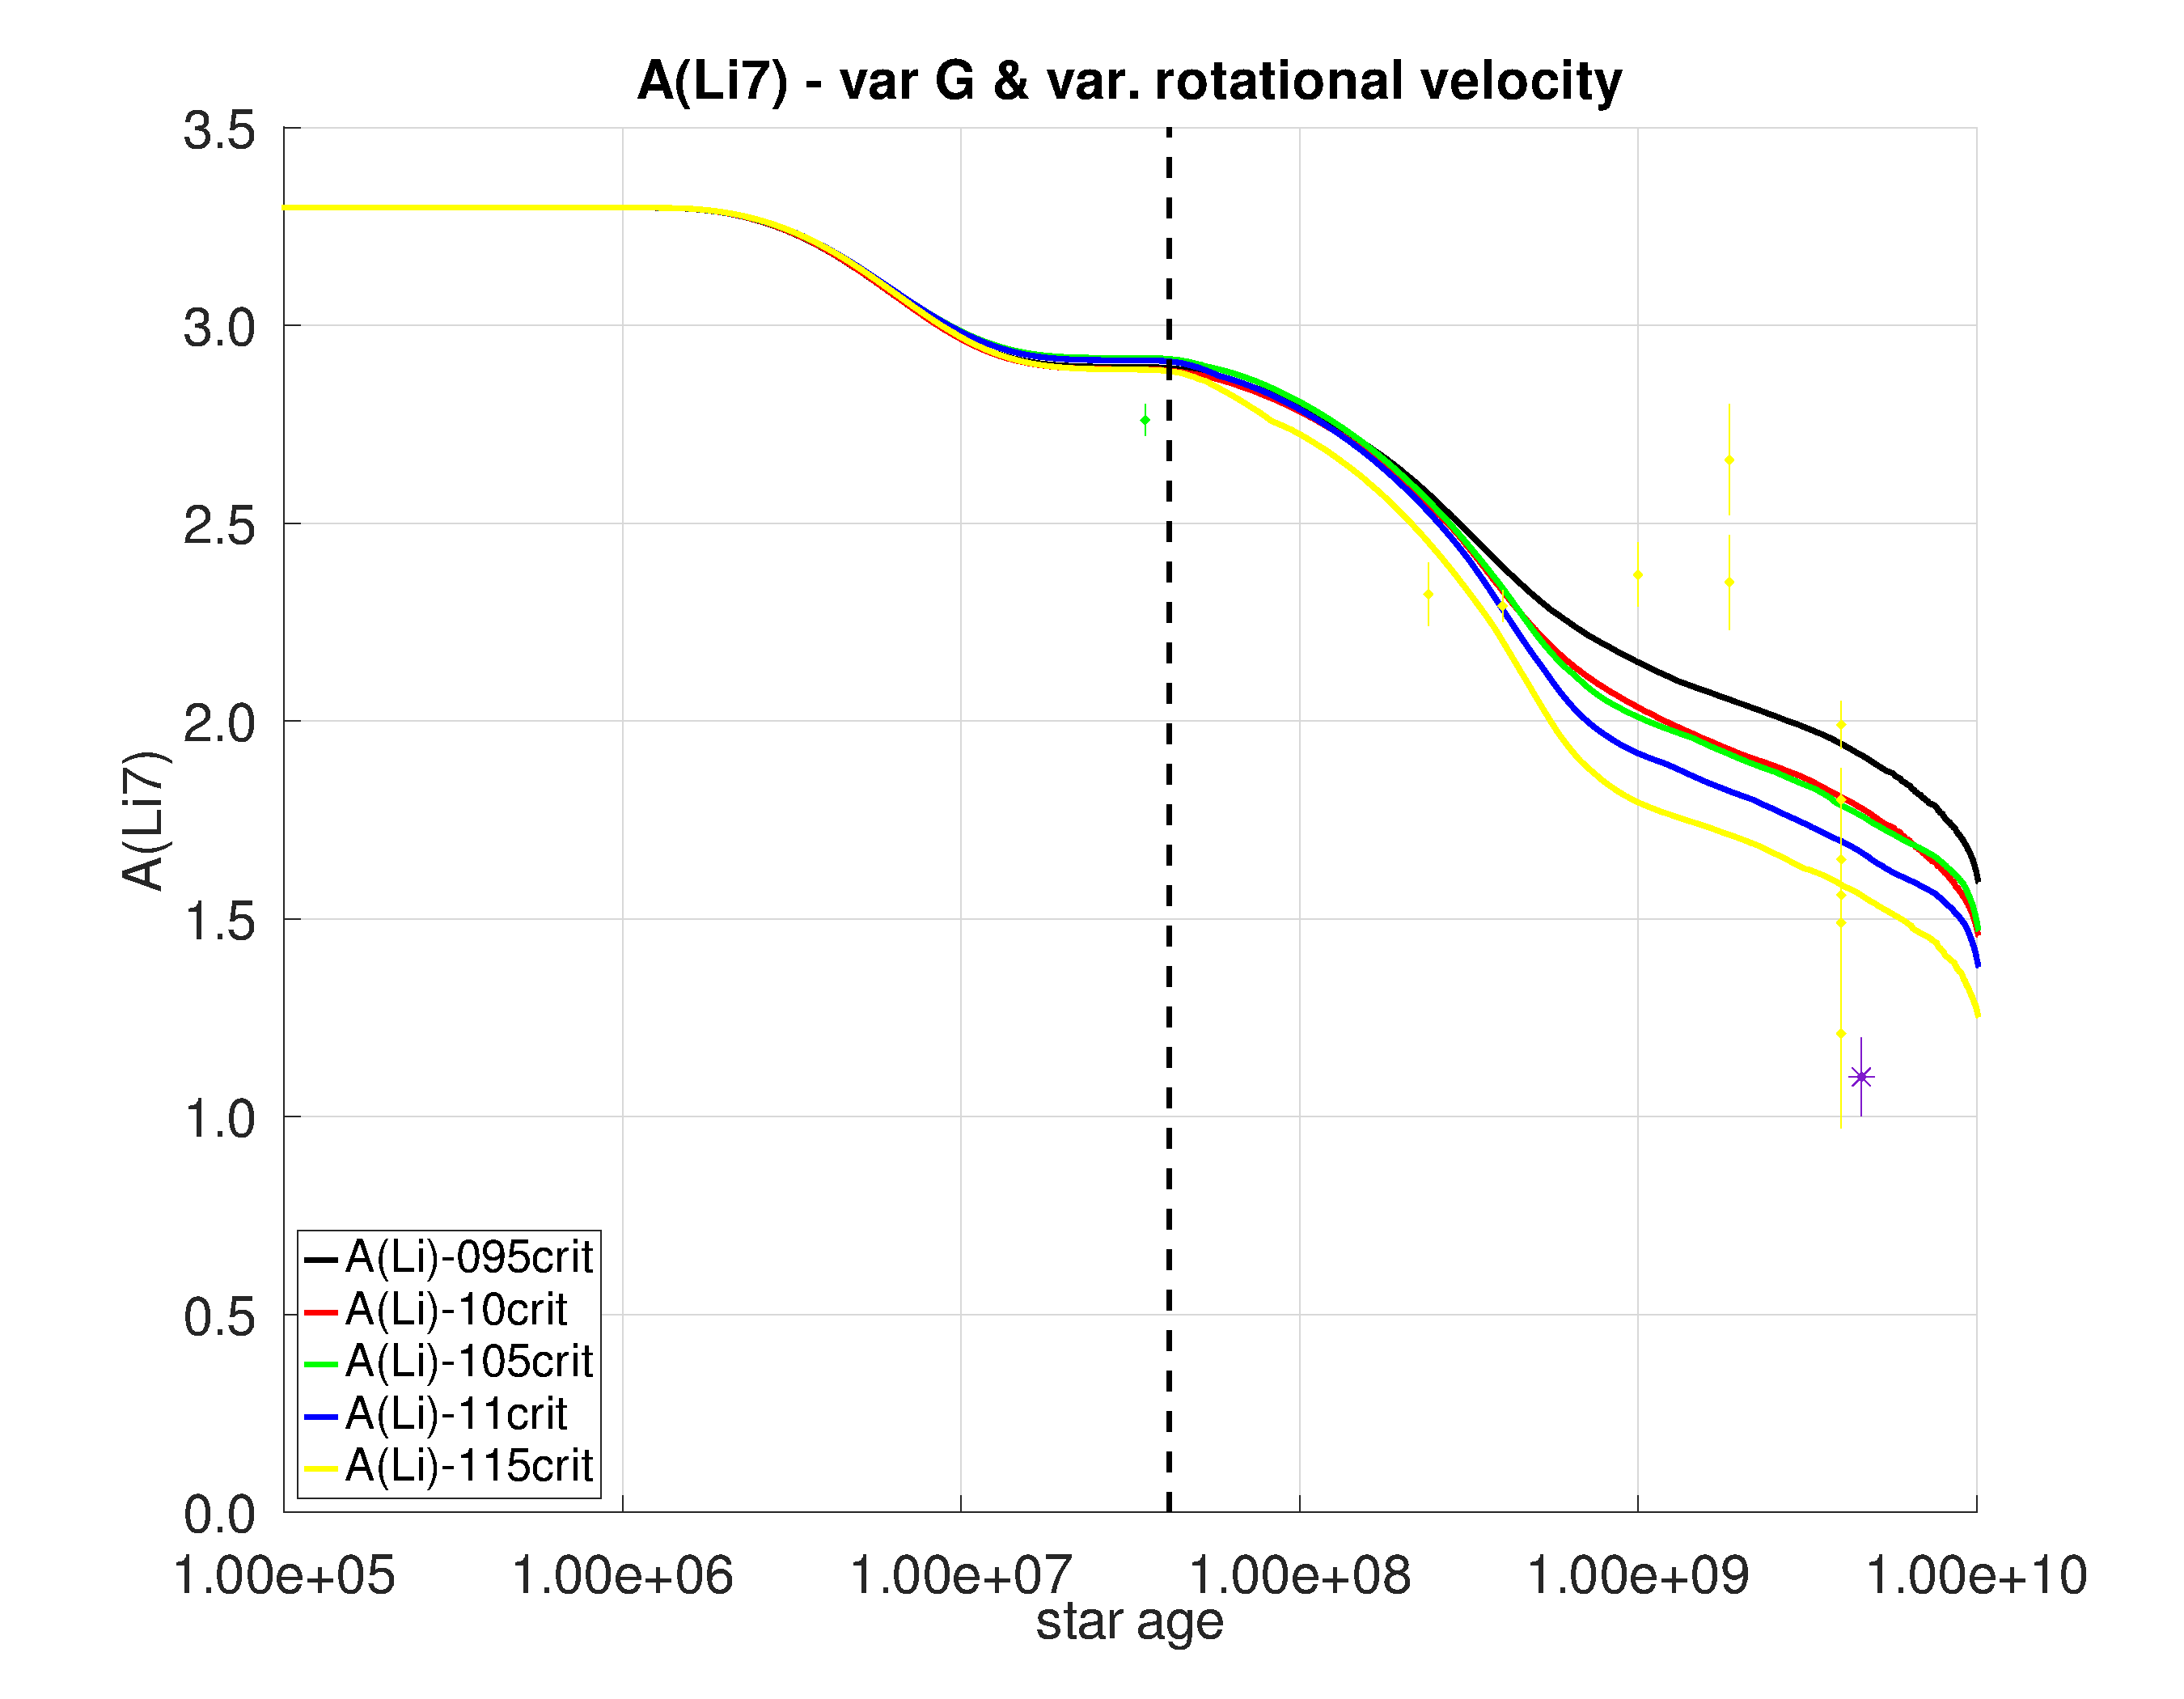
\includegraphics[clip,width=\textwidth]{figures/paper2/li_var_vel_var_g_1.pdf}
    \label{fig:subim11}
    \end{subfigure}
    \begin{subfigure}[h]{0.47\textwidth}
    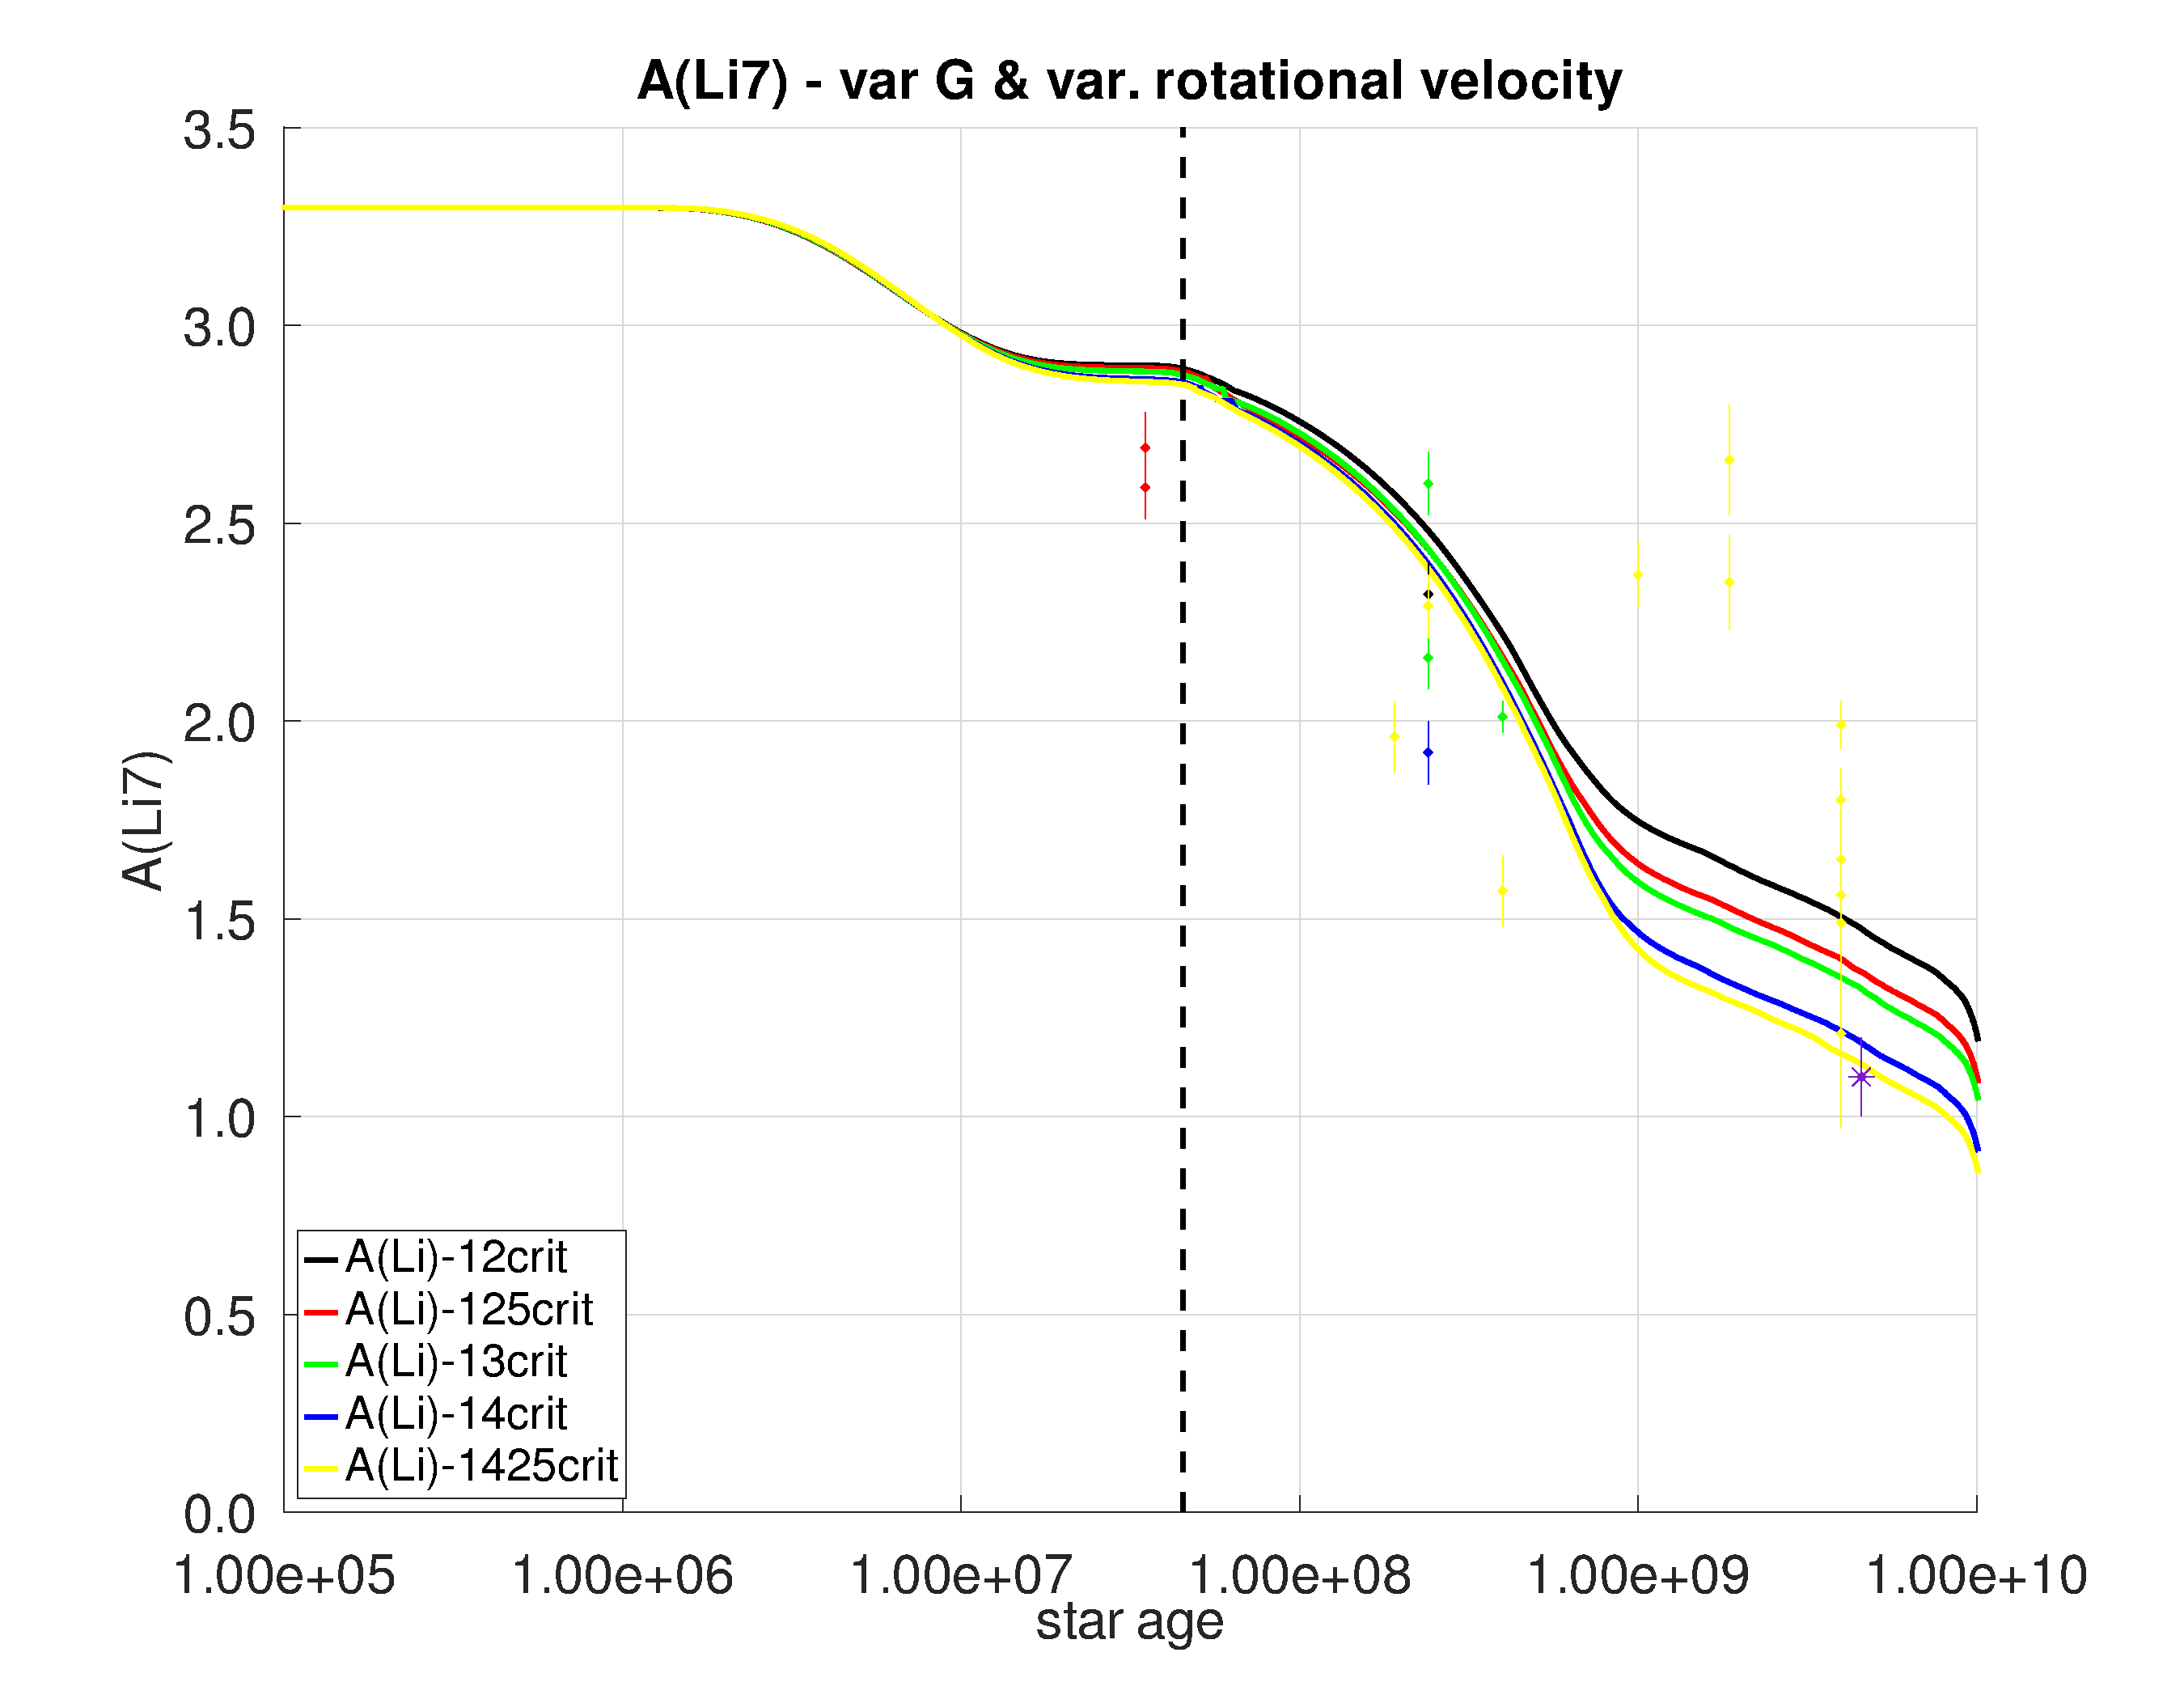
\includegraphics[clip,width=\textwidth]{figures/paper2/li_var_vel_var_g_3.pdf}
    \label{fig:subim12}
    \end{subfigure}
    \begin{subfigure}[h]{0.47\textwidth}
    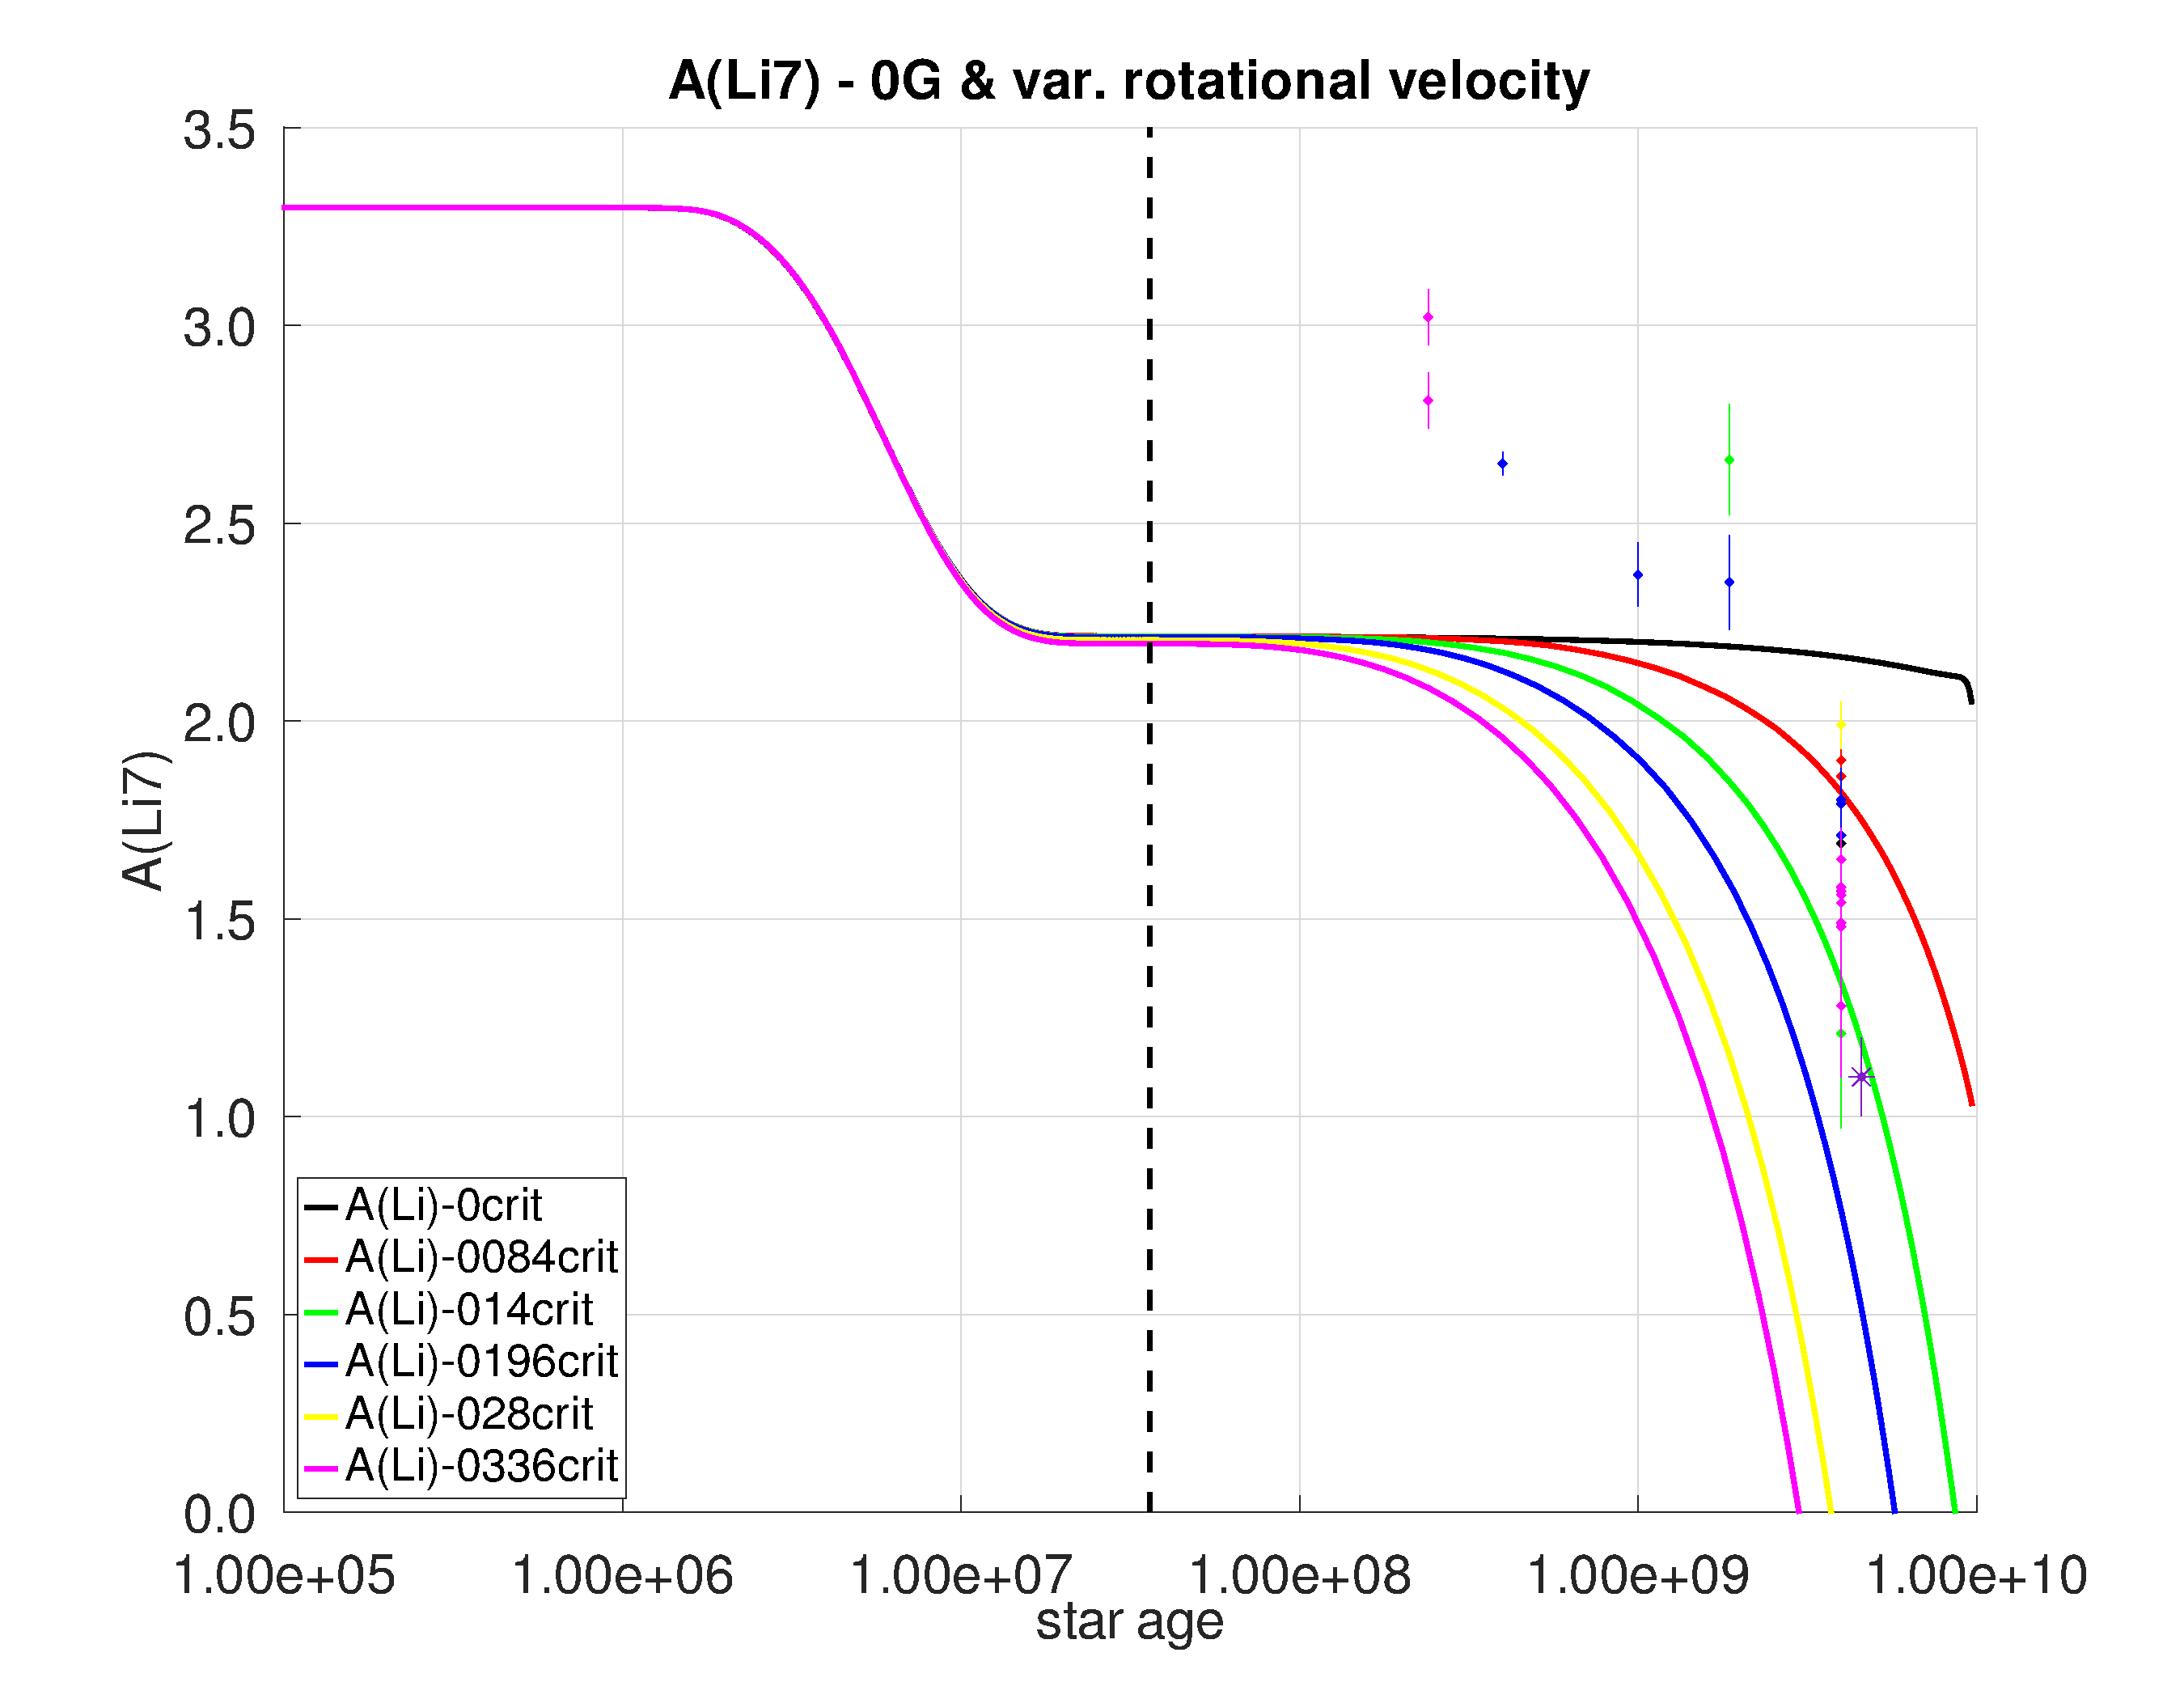
\includegraphics[trim = 25mm 10mm 15mm 10mm, clip,width=\textwidth]{figures/paper2/li_var_vel_0_0g_0.pdf}
    \label{fig:subim13}
    \end{subfigure}
    \begin{subfigure}[h]{0.47\textwidth}
    
\includegraphics[width=\textwidth]{figures/blank.eps}
    \label{fig:subim14}
    \end{subfigure}

\caption{Grid showing the evolution of surface \isotope[7]{Li} abundance relative to \isotope[1]{H}, as a function of time for several 1 $\msun$ models. The top two figures show a set of models with variable magnetic field with intensity, and $\omegaini$ varying between 0.095 and 0.1425. In the bottom one the magnetic field intensity was set to $0.0\,\Gauss$, and $\omegaini$ varying between 0.0 and 0.0336. The purple star is the surface Li abundance for the present-day Sun \citep{Asplund2009}. The dashed vertical line makes reference to the ZAMS.}
\label{fig:grid_li_var_vel}
\end{figure*}
\par


\begin{figure*}
    \centering
    \begin{subfigure}[h]{0.47\textwidth}
    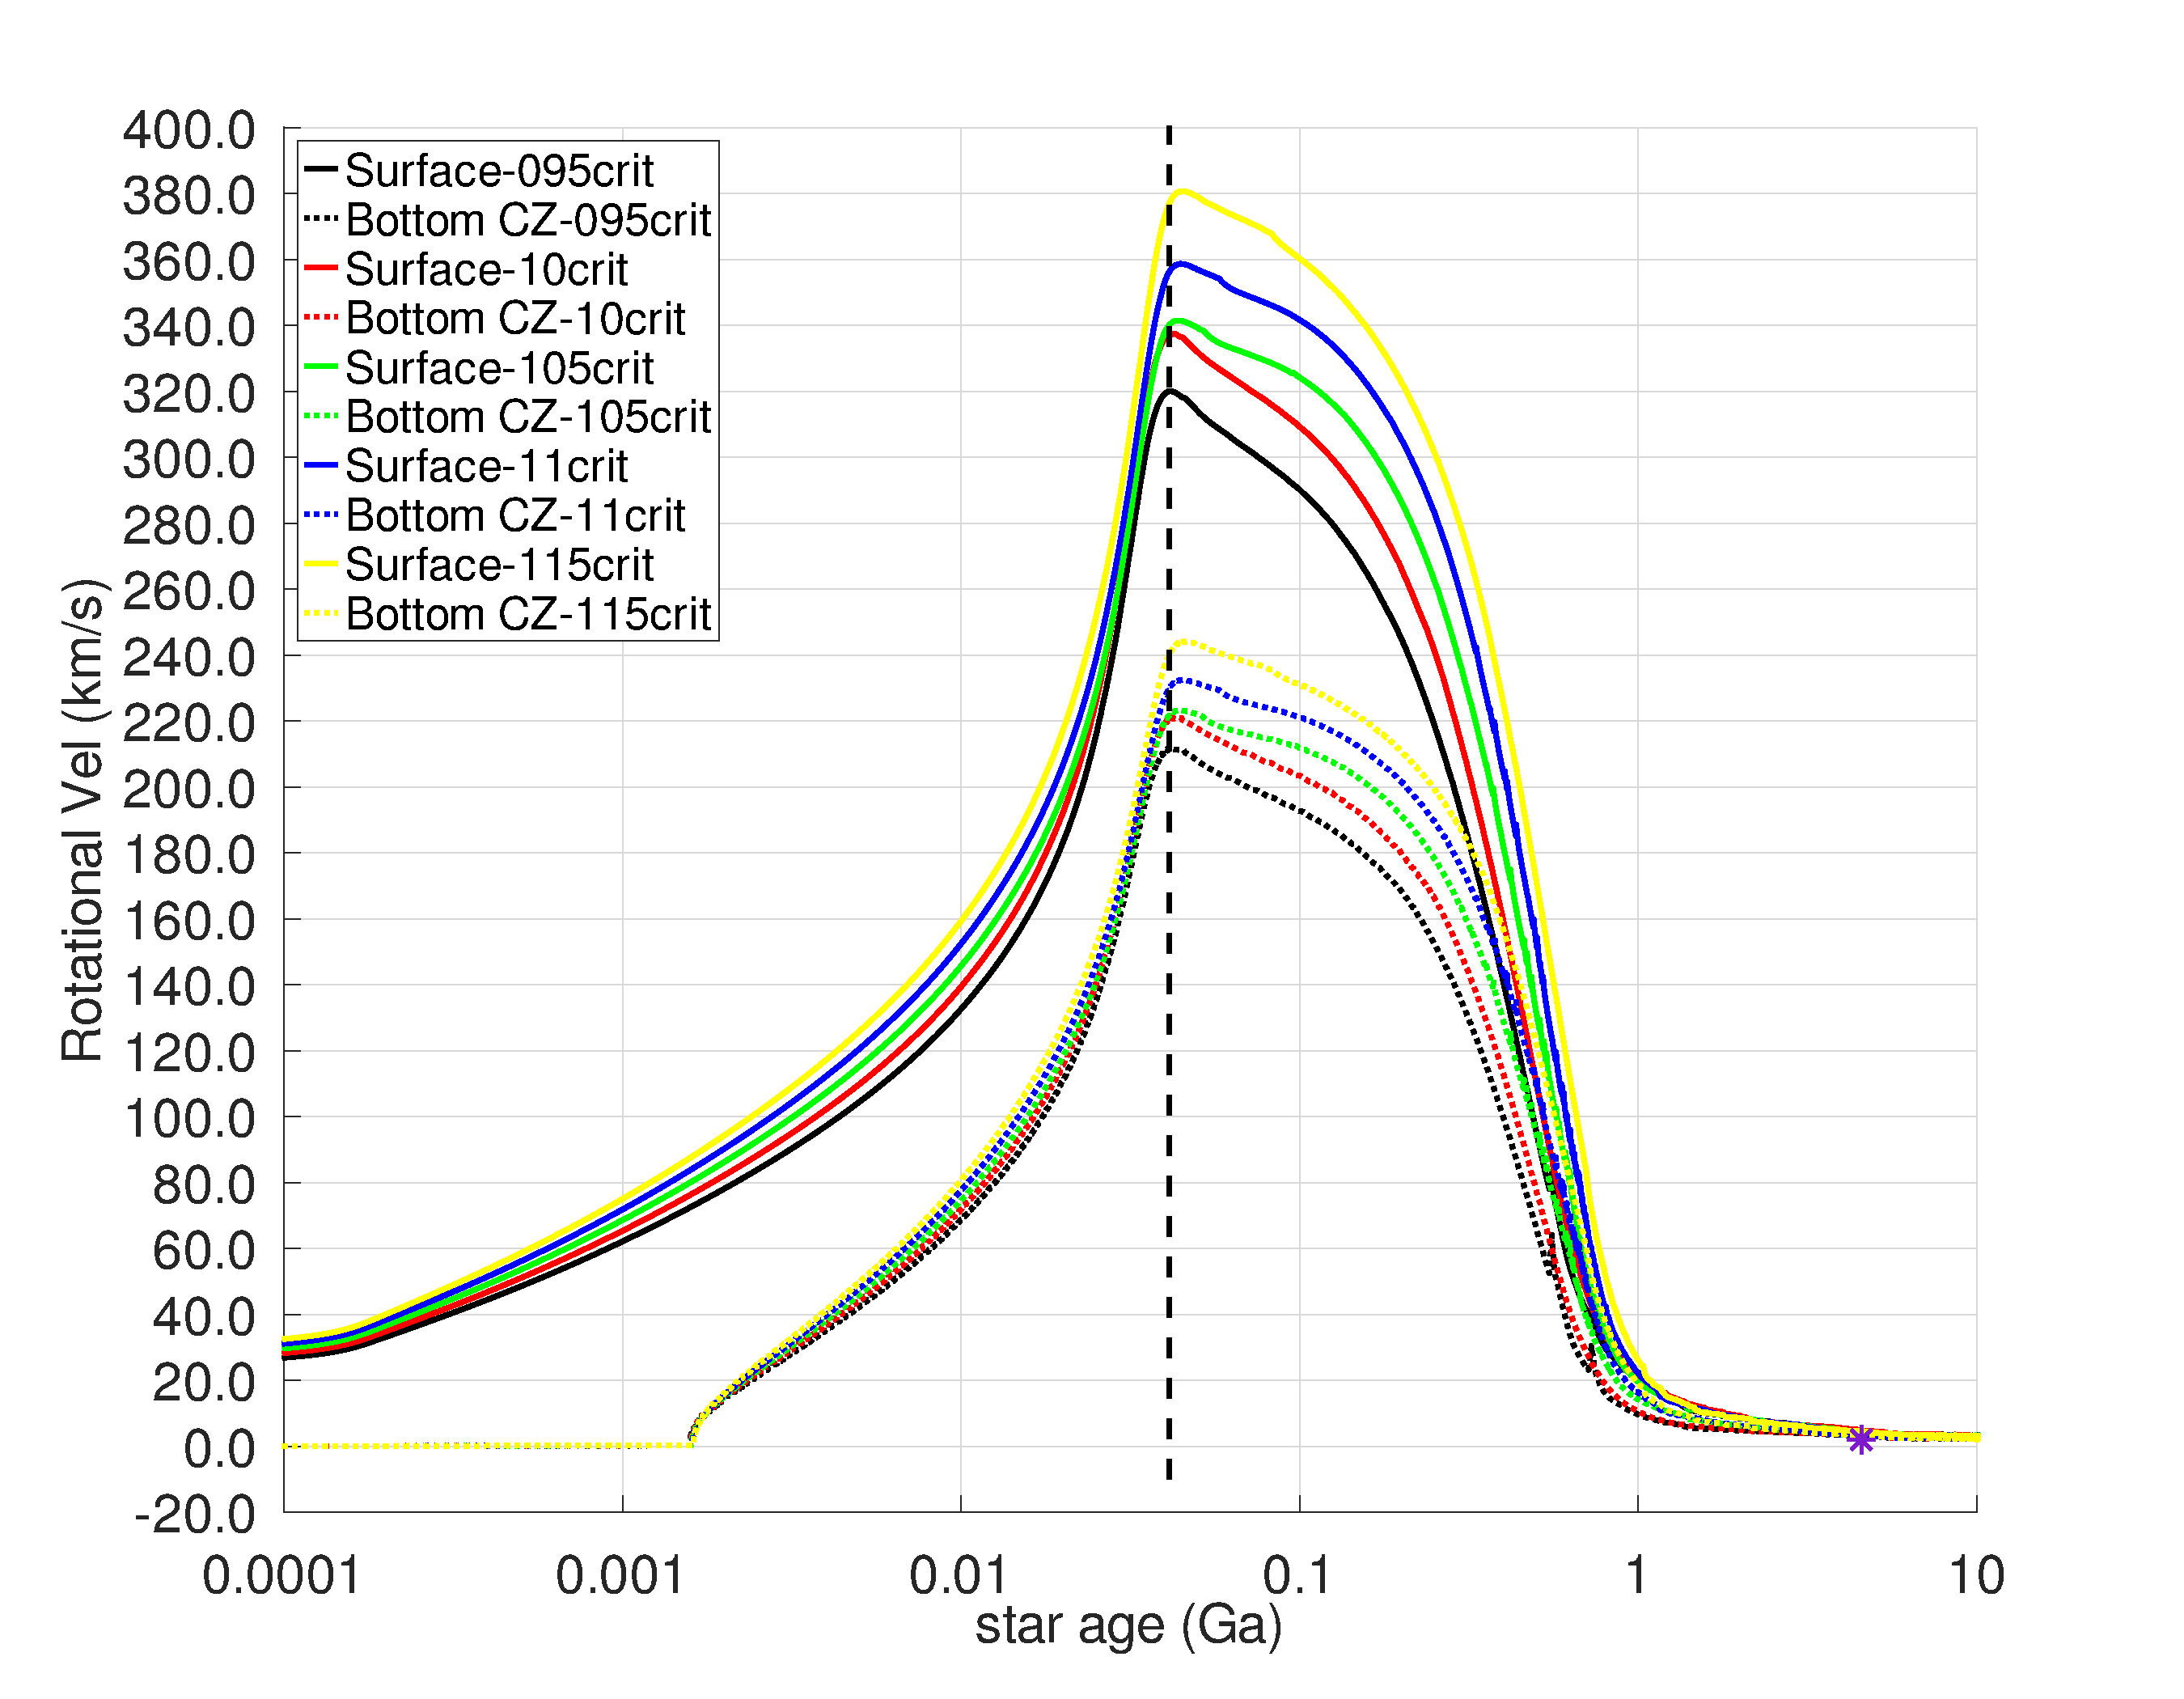
\includegraphics[clip,width=\textwidth]{figures/paper2/rot_vel_var_vel_var_g1.pdf}
    \label{fig:subim21}
    \end{subfigure}
    \begin{subfigure}[h]{0.47\textwidth}
    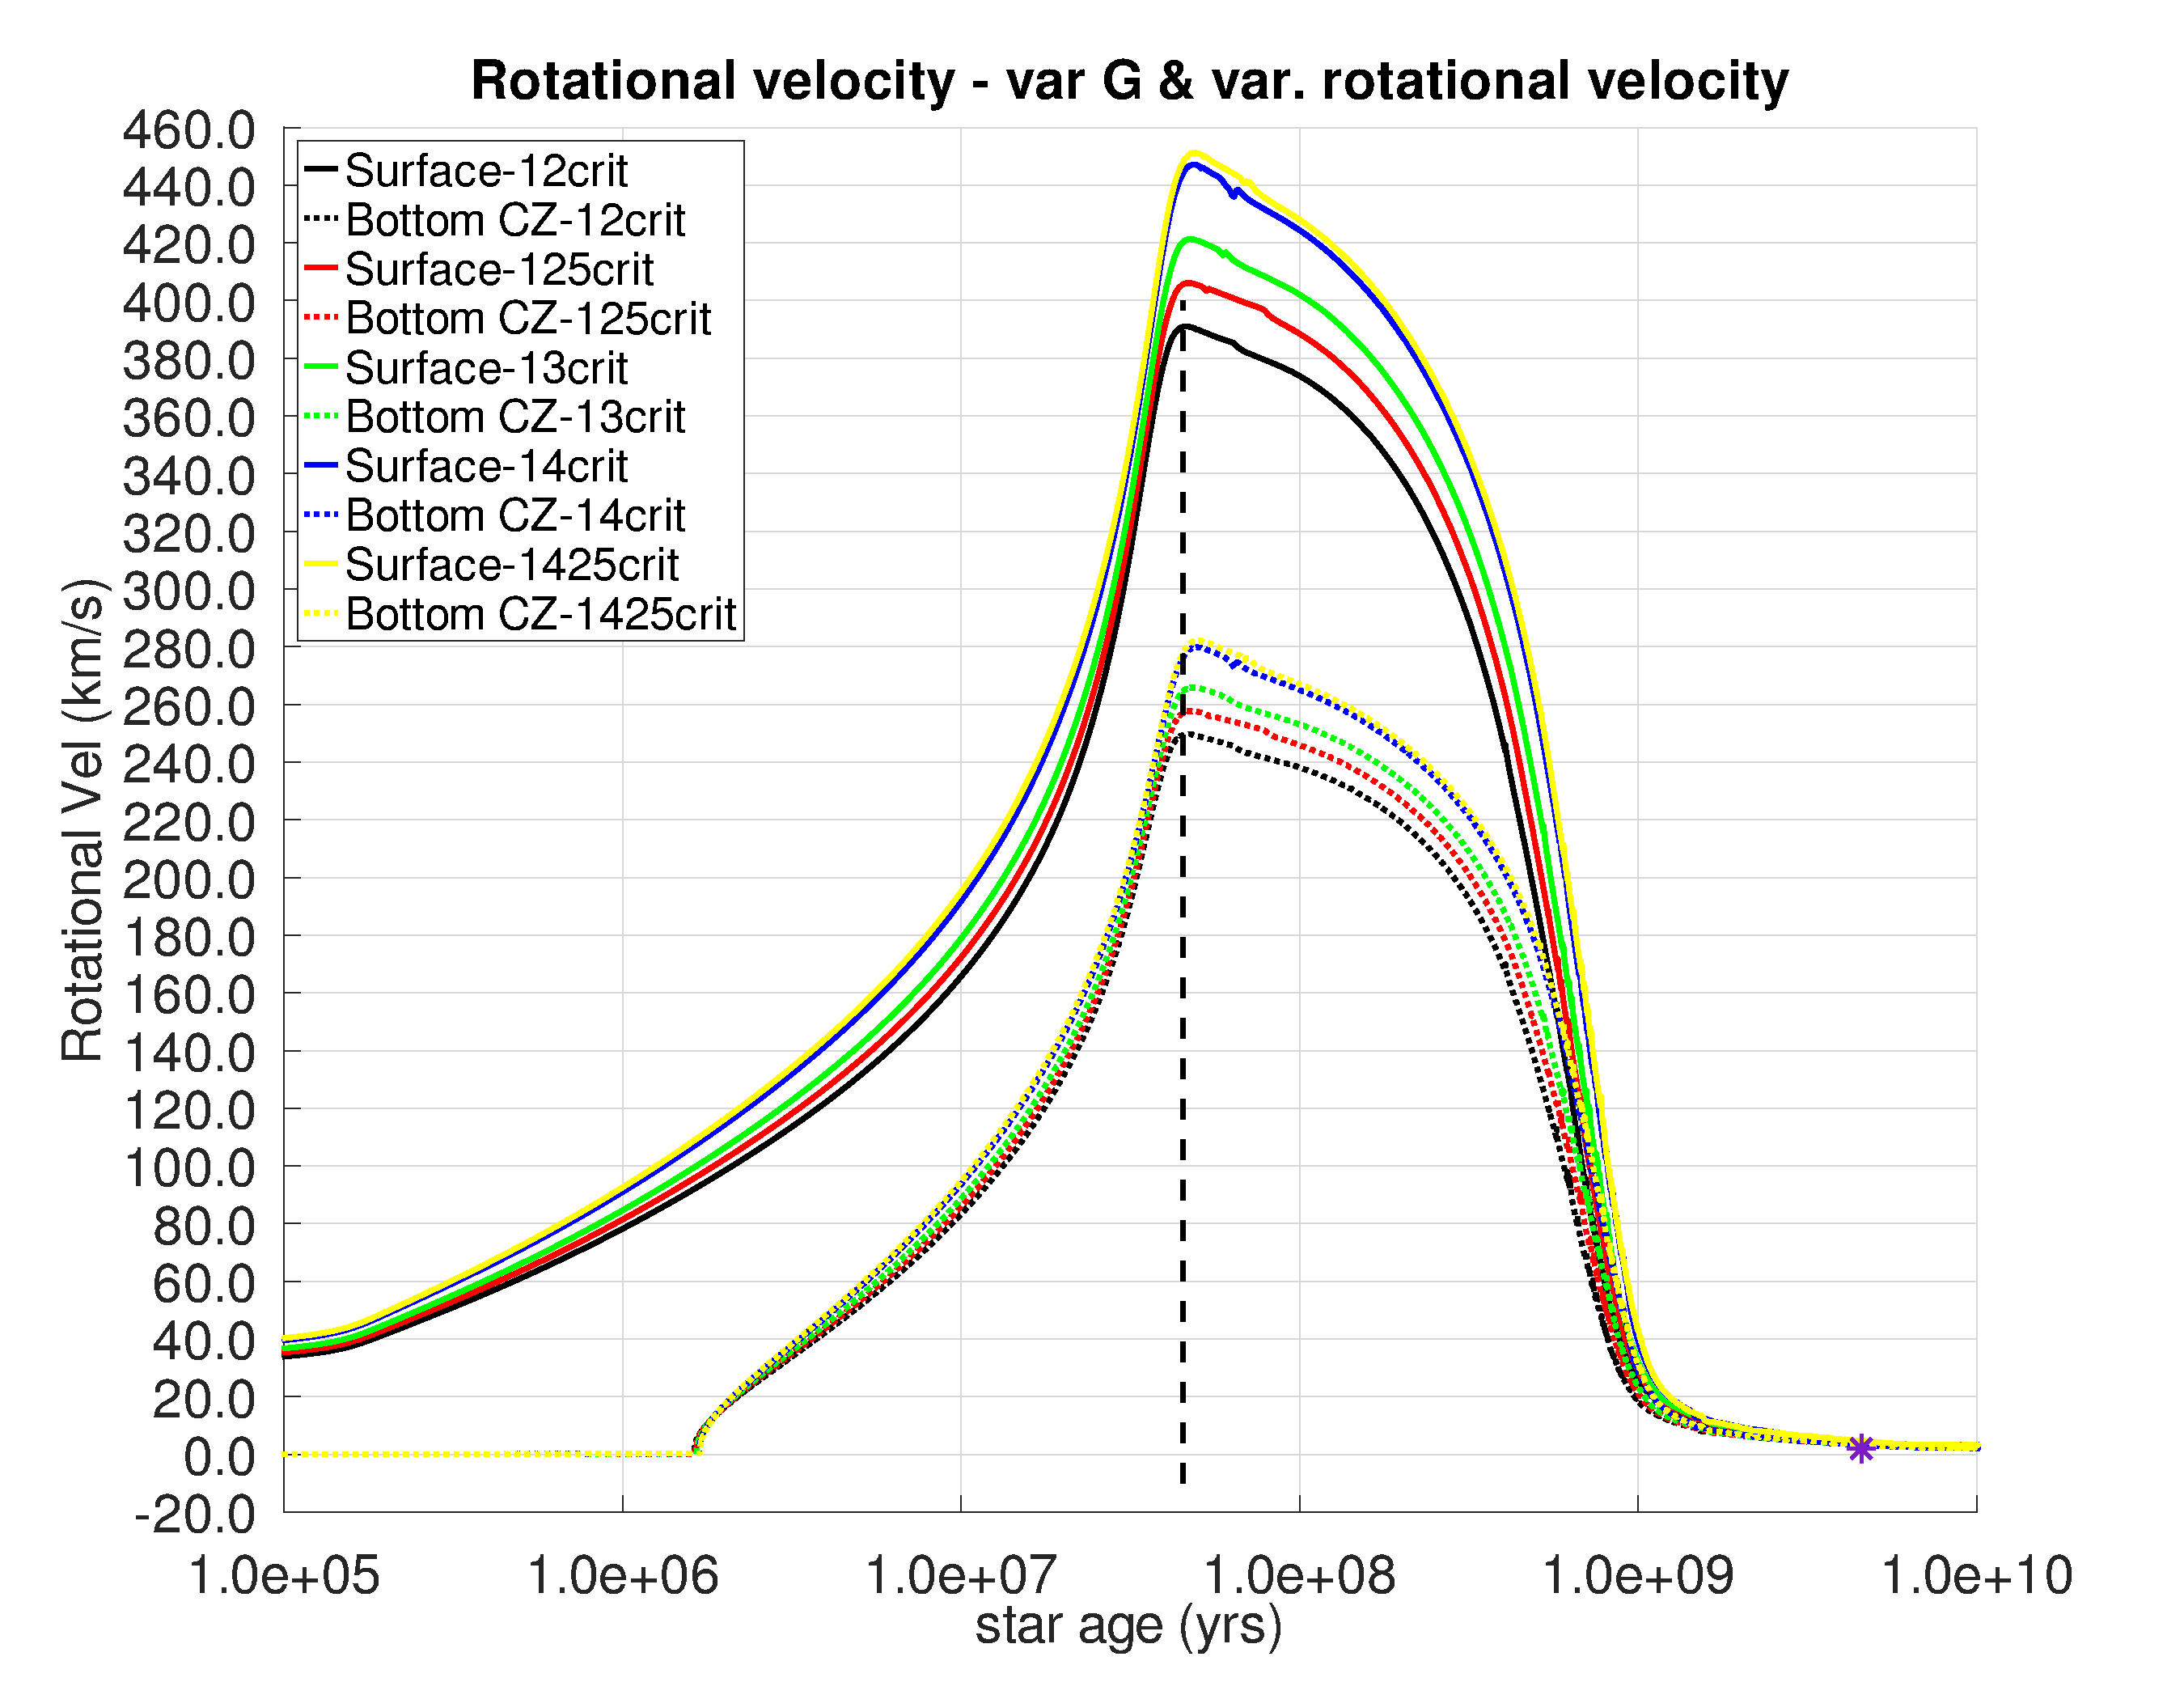
\includegraphics[clip,width=\textwidth]{figures/paper2/rot_vel_var_vel_var_g3.pdf}
    \label{fig:subim22}
    \end{subfigure}
    \begin{subfigure}[h]{0.47\textwidth}
    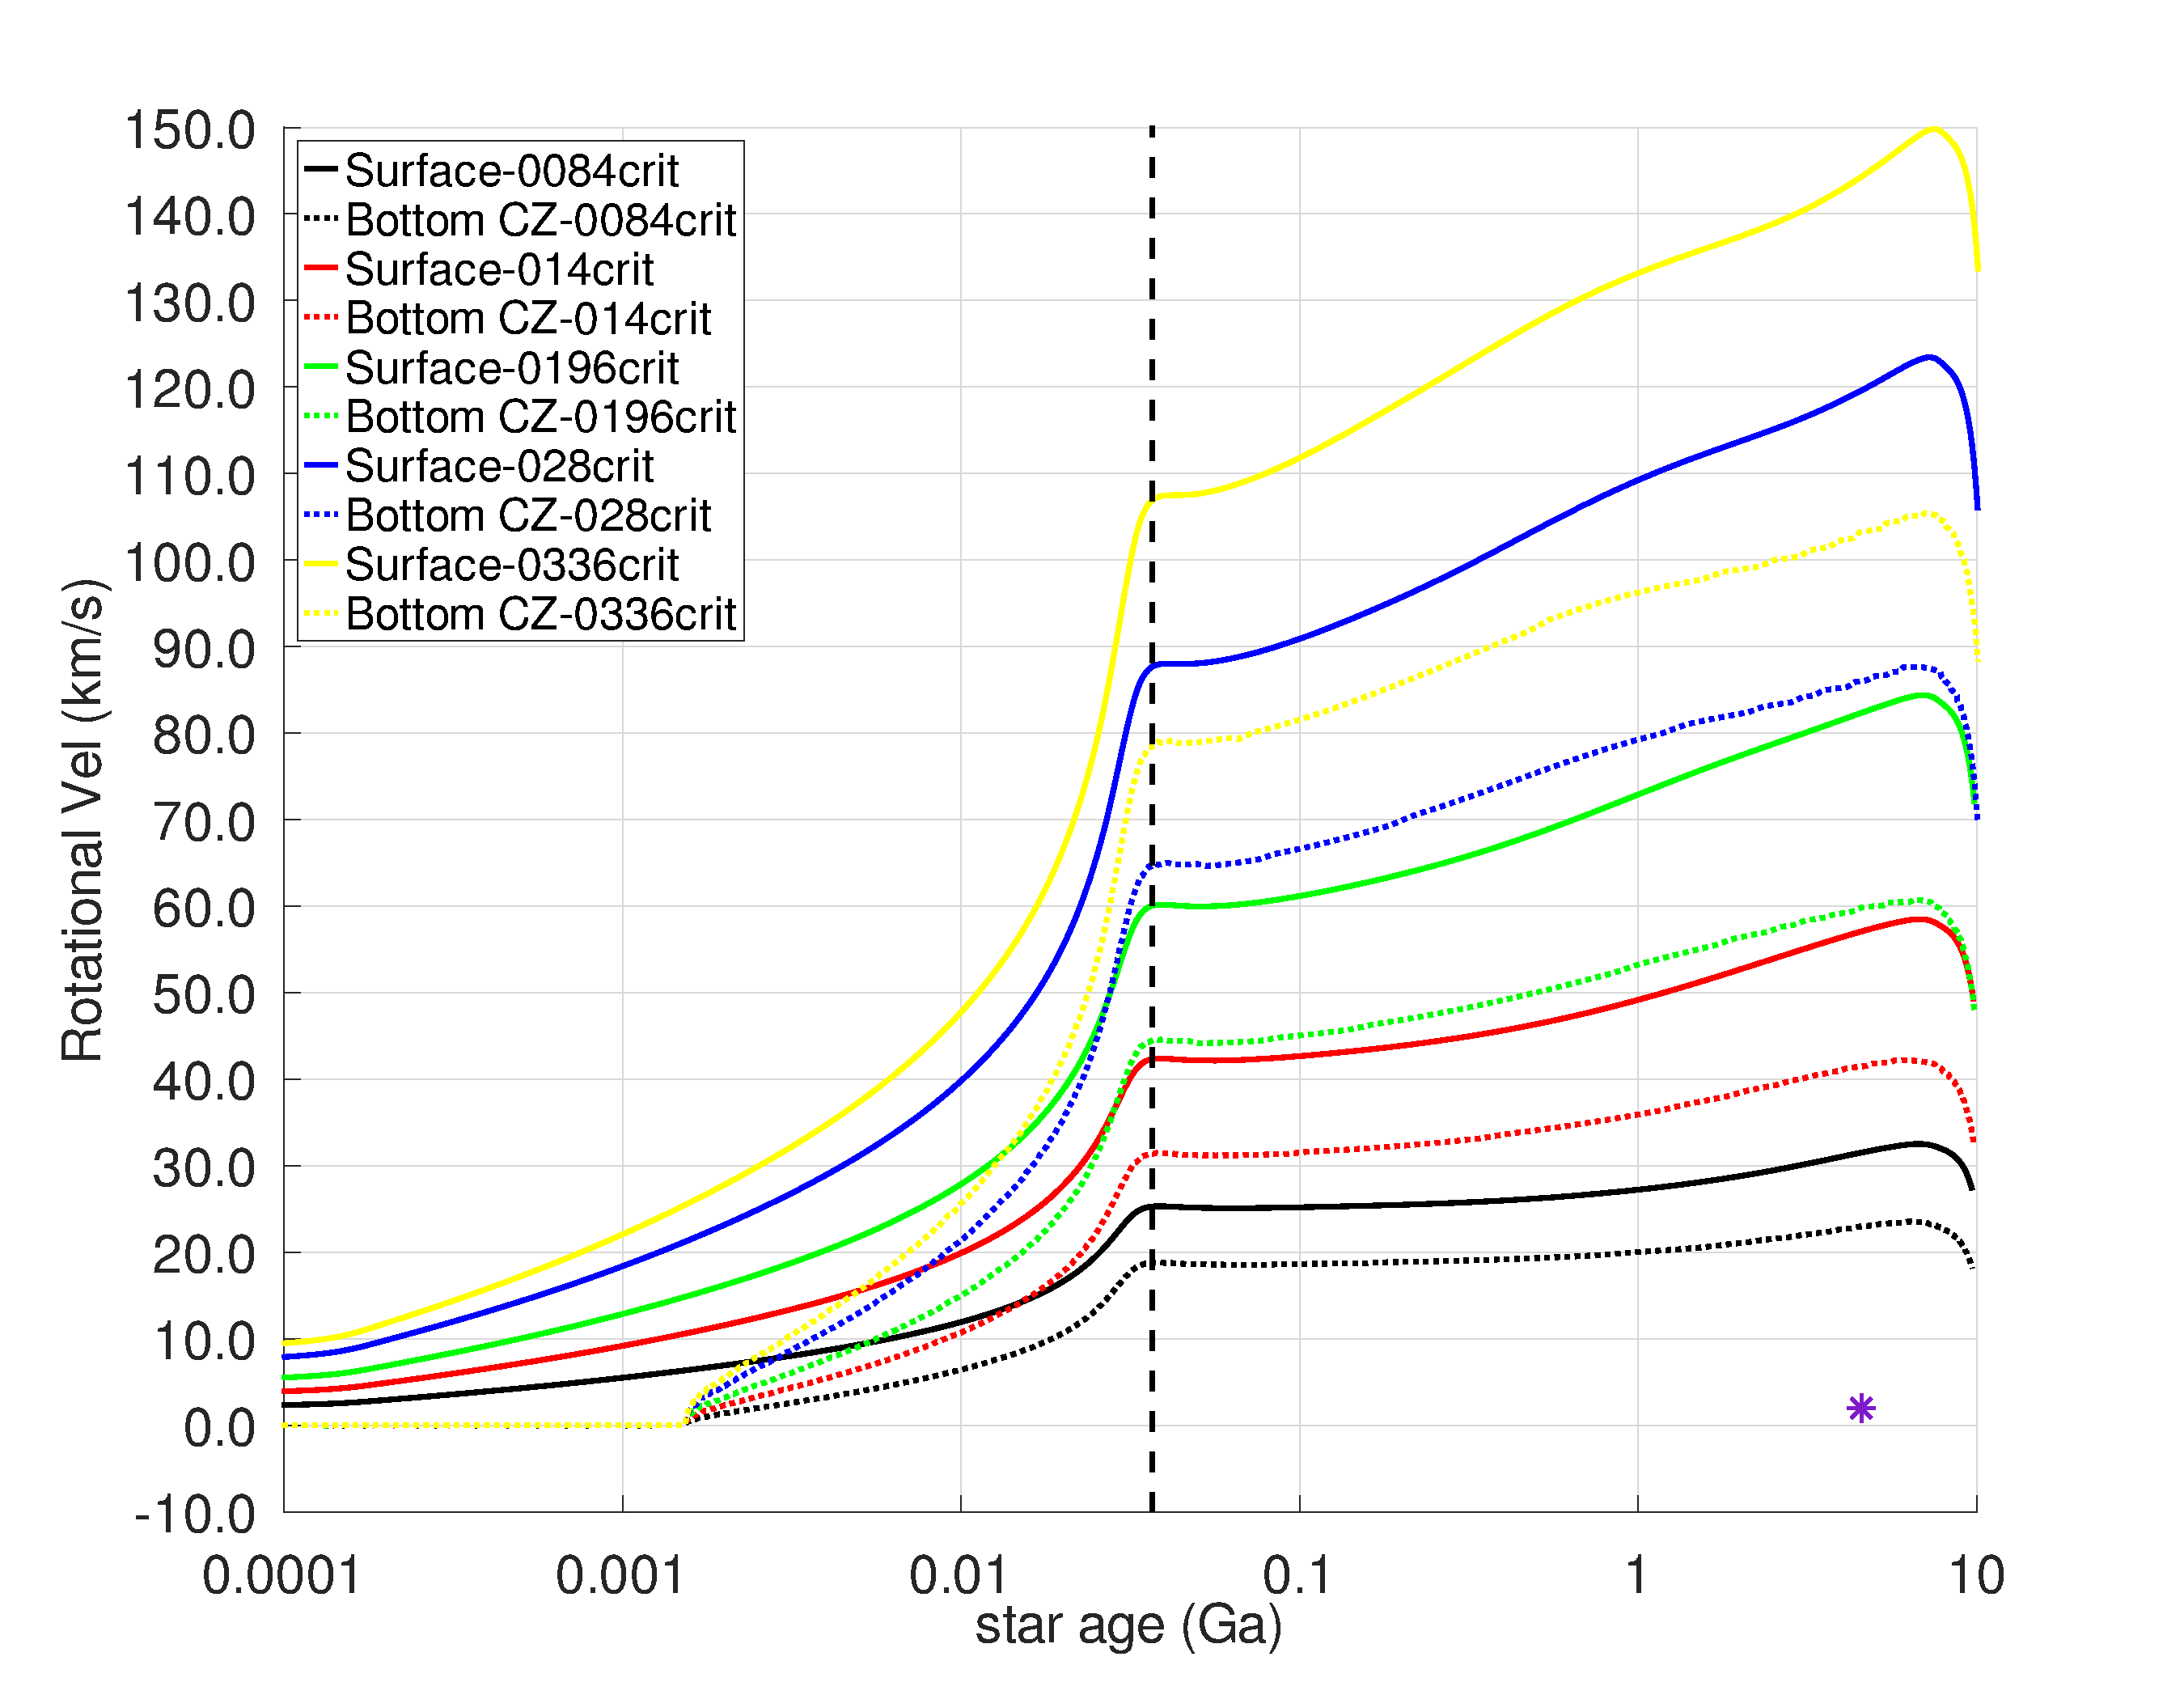
\includegraphics[clip,width=\textwidth]{figures/paper2/rot_vel_var_vel_0_0g_0.pdf}
    \label{fig:subim23}
    \end{subfigure}    
    \begin{subfigure}[h]{0.47\textwidth}
    
\includegraphics[width=\textwidth]{figures/blank.eps}
    \label{fig:subim24}
    \end{subfigure}
\caption{Grid showing of the evolution of surface rotational velocity, as a function of time for several 1 $\msun$ models. The top two figures show a set of models with variable magnetic field with intensity, and $\omegaini$ varying between 0.095 and 0.1425. In the bottom one the magnetic field intensity was set to $0.0\,\Gauss$, and $\omegaini$ varying between 0.0 and 0.0336. The purple star and square are surface Li abundance for the present-day Sun \citep{Asplund2009}. The dashed vertical line makes reference to the ZAMS.}
\label{fig:grid_li_var_g}
\end{figure*}

\begin{figure*}
    \centering
    \begin{subfigure}[h]{0.47\textwidth}
    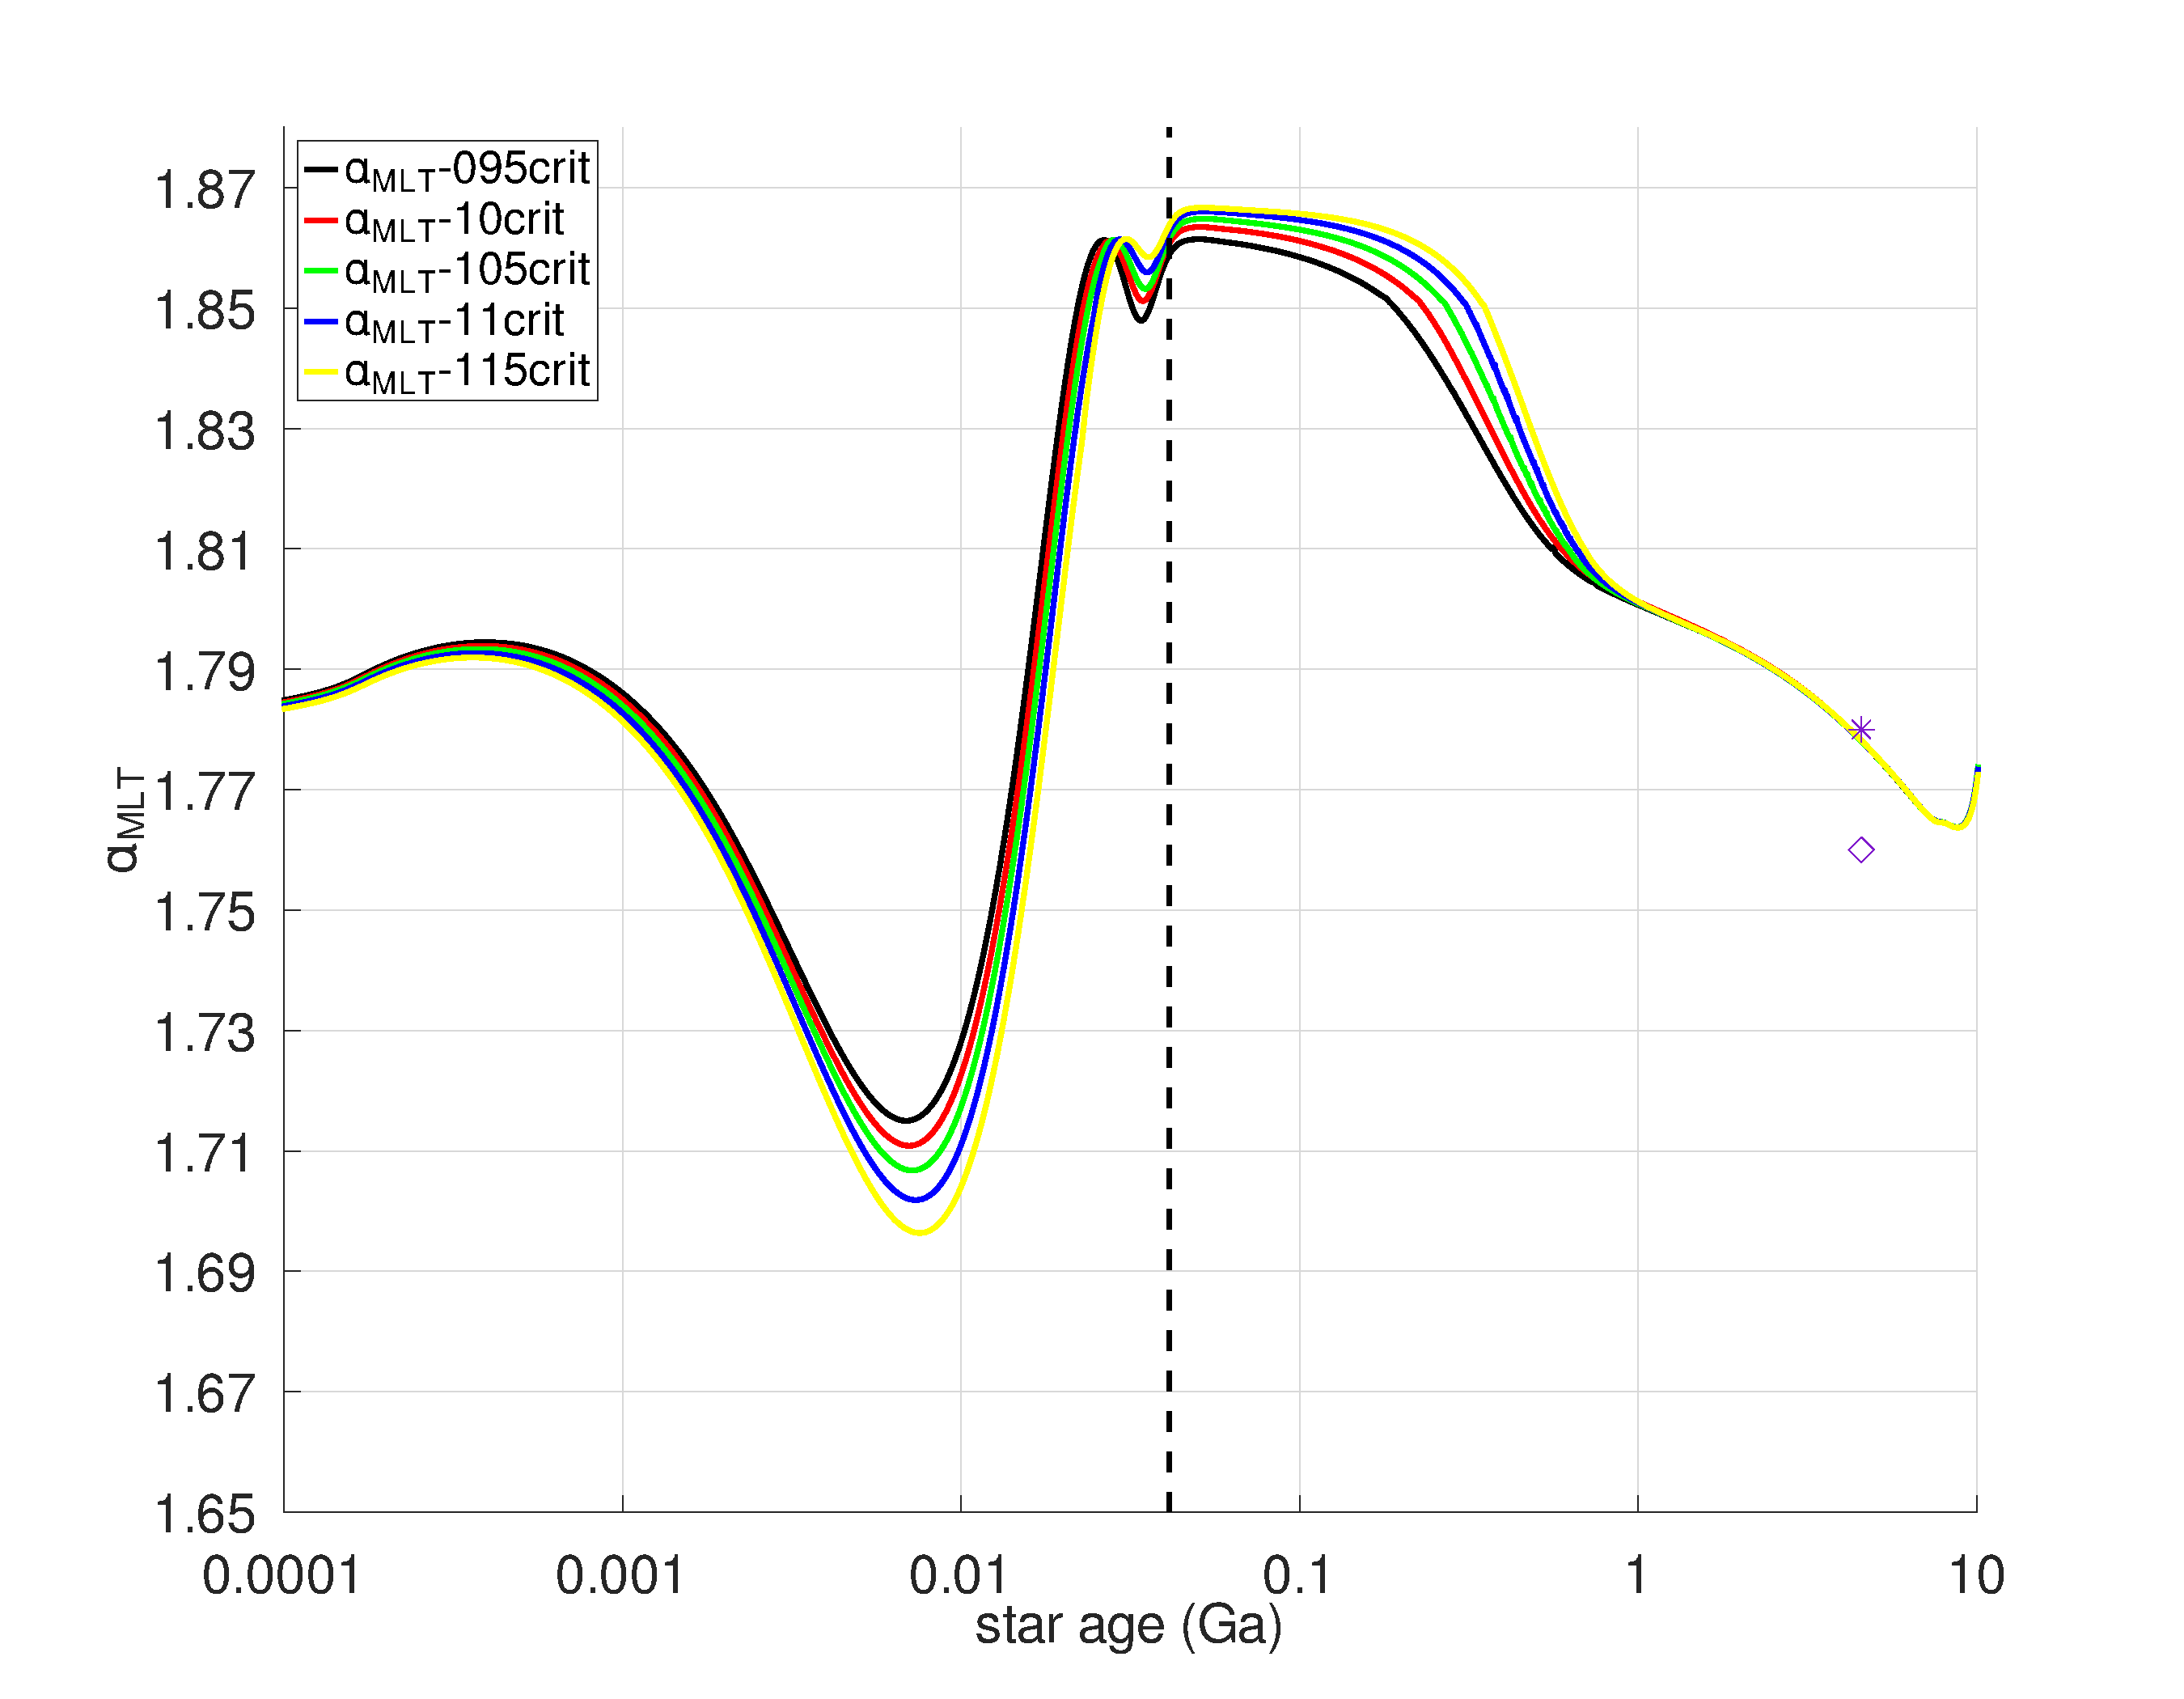
\includegraphics[clip,width=\textwidth]{figures/paper2/alpha_mlt_var_vel_g1.pdf}
    \label{fig:subim41}
    \end{subfigure}
    \begin{subfigure}[h]{0.47\textwidth}
    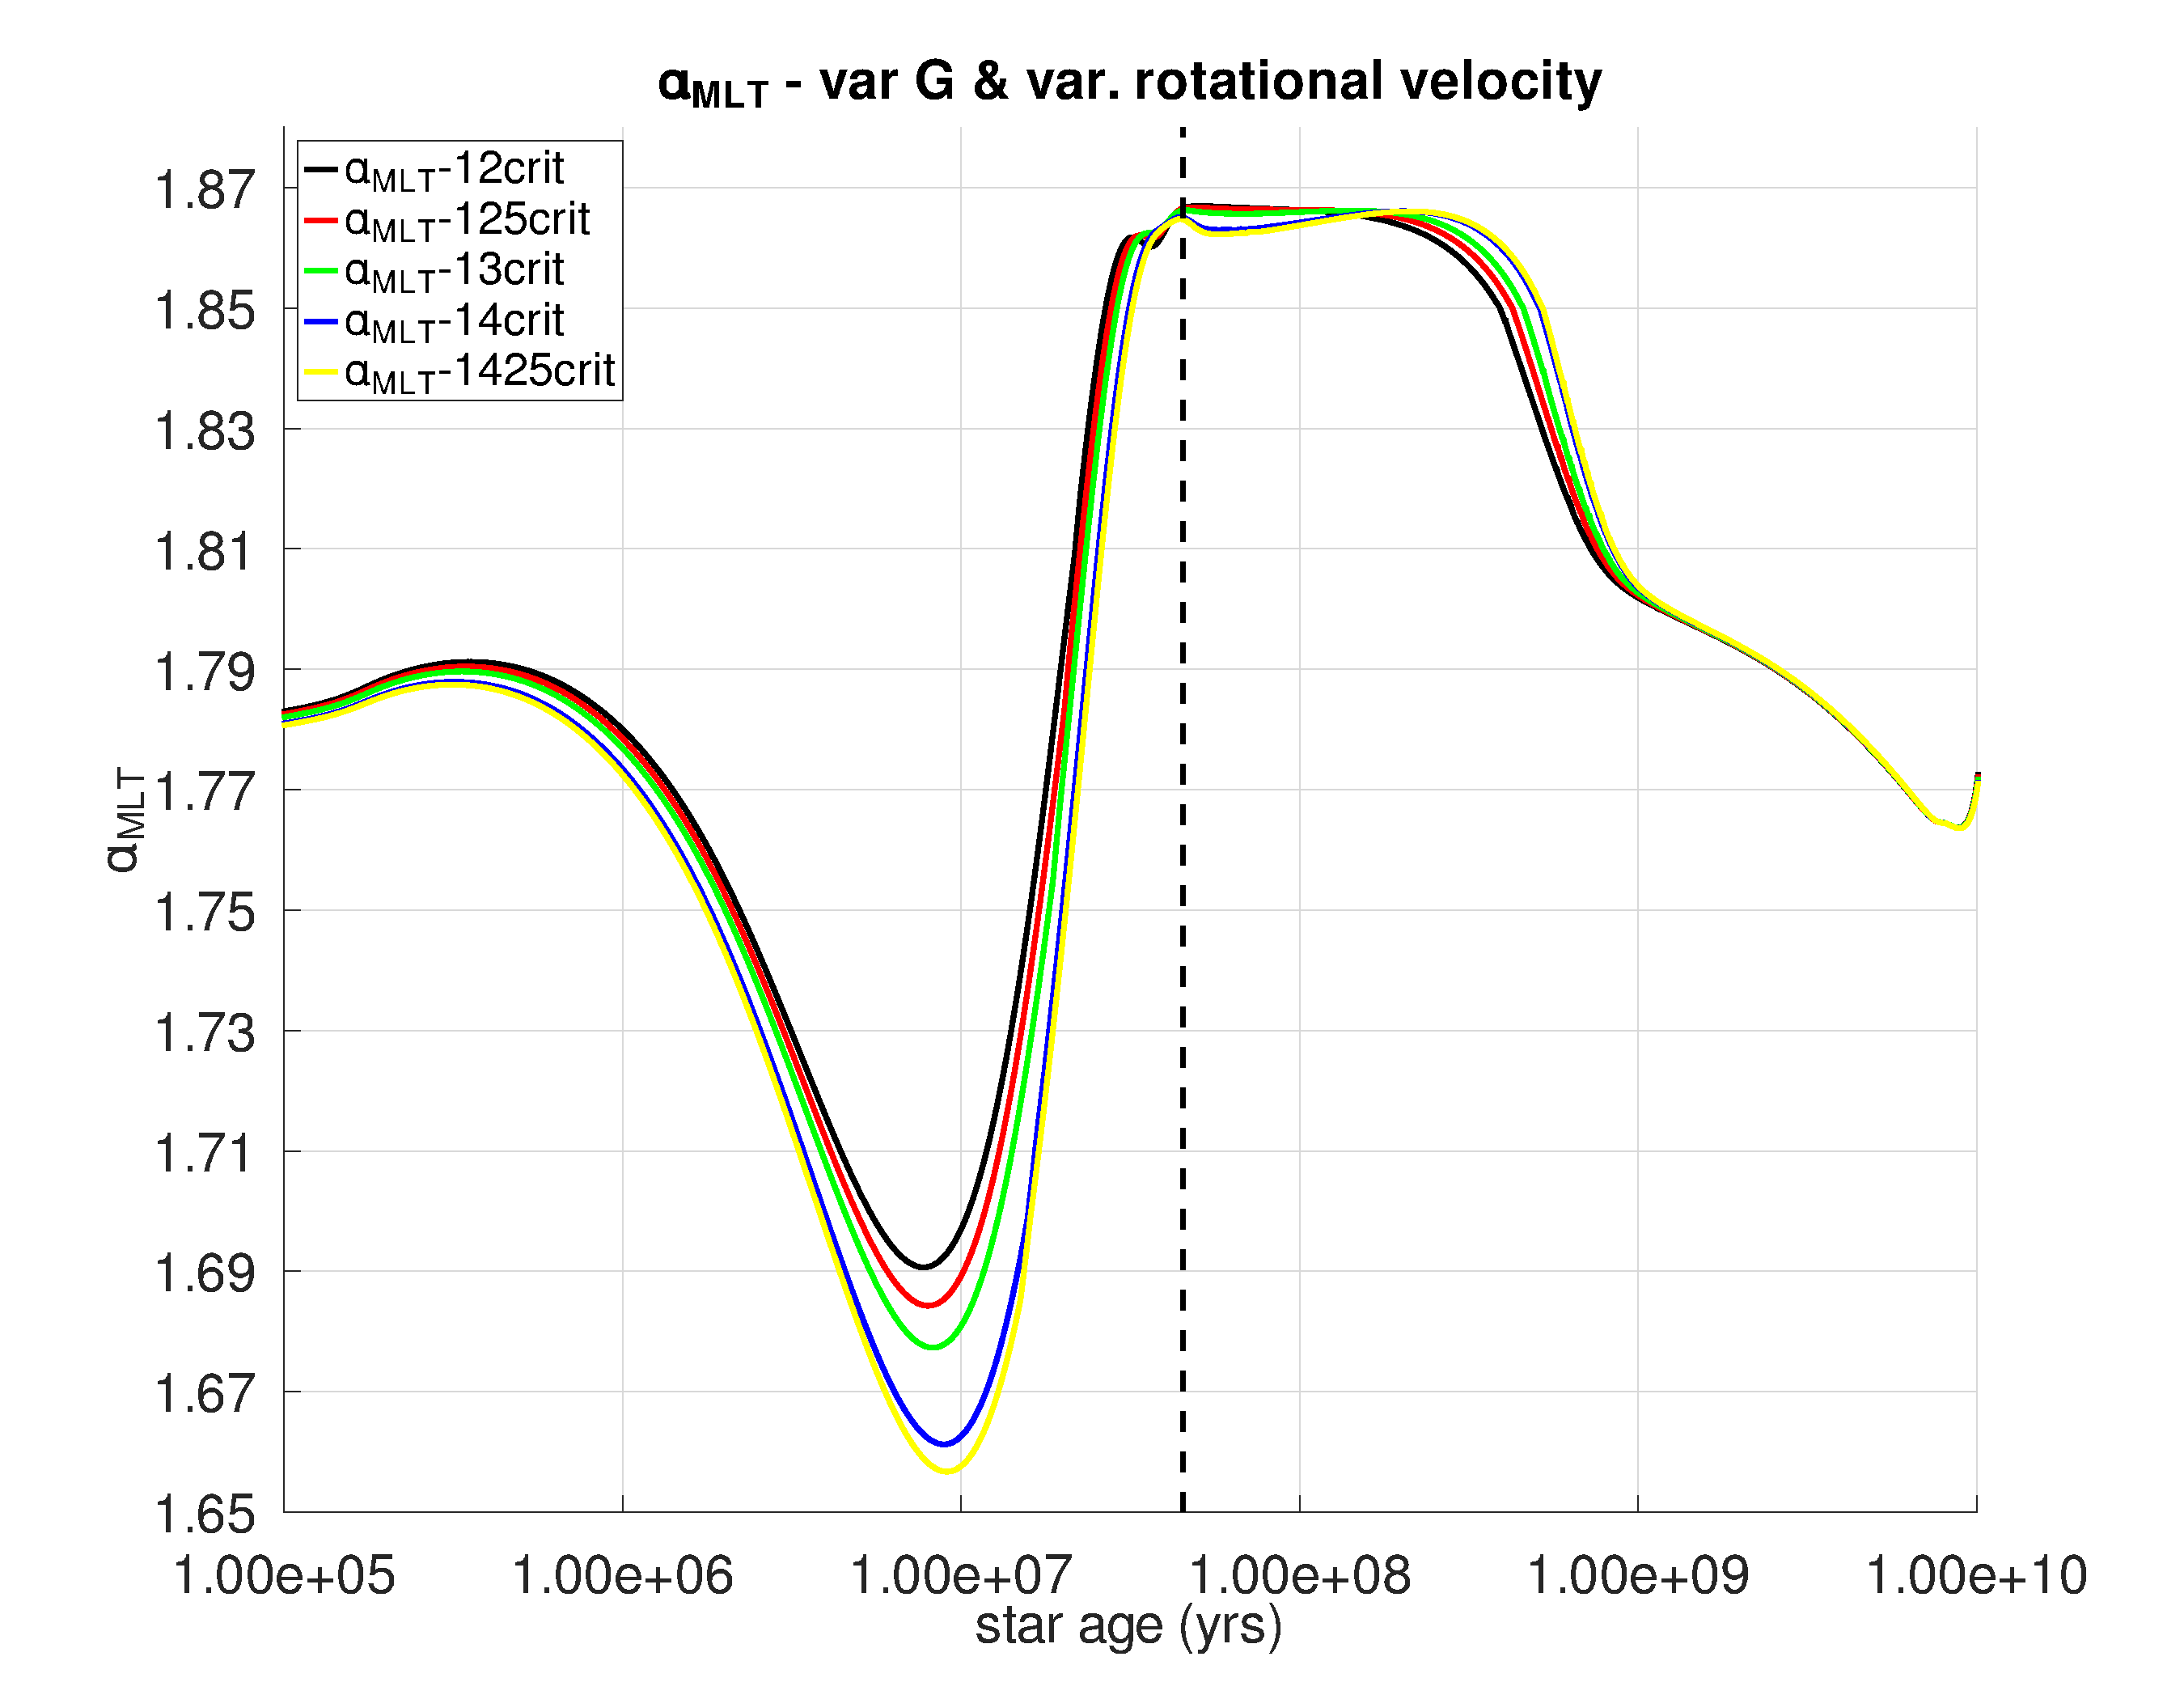
\includegraphics[clip,width=\textwidth]{figures/paper2/alpha_mlt_var_vel_g3.pdf}
    \label{fig:subim42}
    \end{subfigure}
\caption{Grid showing of the evolution of $\amlt$, as a function of time for several 1 $\msun$ models. The two figures show a set of models with variable magnetic field with intensity, and $\omegaini$ varying between 0.095 and 0.1425. The purple star and diamond are the $\amlt$ given by \citet{Sonoi2018} and \citet{Samadi2005}, respectively. The dashed vertical line makes reference to the ZAMS.}
\label{fig:grid_rot_vel}
\end{figure*}

\appendix
%%%%%%%%%%%%%%%%%%%%%%%%%%%%%%%%%%%%%%%%%%%%%%%%%%



% Don't change these lines
\bsp	% typesetting comment
\label{lastpage}
\end{document}

% End of mnras_template.tex